% !TeX program = xelatex
\documentclass[11pt,a4paper,UTF8,scheme=plain,fontset=fandol]{ctexbook}

% ---------- Page setup ----------
\usepackage[margin=2.5cm]{geometry}
\usepackage{setspace}
\setstretch{1.2}
\usepackage{fancyhdr}

% ---------- Math & physics ----------
\usepackage{amsmath,amssymb,amsfonts,amsthm,mathtools}
\usepackage{bm}          % bold math symbols
\usepackage{physics}     % \dv, \pdv, \qty, \vb, \comm, ...
\usepackage{siunitx}     % SI units
\usepackage{braket}      % Dirac notation
\usepackage{tensor}      % tensor indices
\usepackage{cancel}      % cancel terms in equations
\usepackage{slashed}     % Feynman slash notation

% ---------- Figures & tables ----------
\usepackage{graphicx}
\usepackage{booktabs}
\usepackage{caption}

% ---------- Links & references ----------
\usepackage[colorlinks=true,linkcolor=blue,citecolor=teal,urlcolor=magenta]{hyperref}
\usepackage[nameinlink]{cleveref}

% ---------- Lists ----------
\usepackage{enumitem}
\setlist[itemize]{leftmargin=2em}

% ---------- Theorem environments ----------
\theoremstyle{definition}
\newtheorem{definition}{Definition}[section]
\newtheorem{example}[definition]{Example}
\newtheorem{exercise}[definition]{Exercise}

\theoremstyle{plain}
\newtheorem{theorem}[definition]{Theorem}
\newtheorem{lemma}[definition]{Lemma}
\newtheorem{proposition}[definition]{Proposition}
\newtheorem{corollary}[definition]{Corollary}

\theoremstyle{remark}
\newtheorem{remark}[definition]{Remark}

% ---------- Page style: footer page numbers only ----------
\pagestyle{fancy}
\fancyhf{}
\fancyfoot[C]{\thepage}
\renewcommand{\headrulewidth}{0pt}
\renewcommand{\footrulewidth}{0pt}
\fancypagestyle{plain}{
  \fancyhf{}
  \fancyfoot[C]{\thepage}
  \renewcommand{\headrulewidth}{0pt}
  \renewcommand{\footrulewidth}{0pt}
}

% ---------- Metadata ----------
\title{Physics Research Note1}
\author{Jizheng Bo}
\date{\today}

\begin{document}
\maketitle
\tableofcontents
\newpage

\chapter{Proton Decay的Bayesian计算}

考虑形变势能:
\begin{equation}
    V(r,\theta)=V_N(r,\theta)+V_c(r,\theta)+V_{so}(r,\theta)+\frac{\hbar^2}{2\mu r^2}(l+\frac{1}{2})^2
\end{equation}

\begin{equation}
    V_N(r,\theta)=-\frac{V_{N0}}{1+\exp\{r-R_N(\theta)/a_N(\theta)\}}
\end{equation}

\begin{equation}
    R_N(\theta)=R_{N0}(1+\beta_2Y_{20}(\theta)+\beta_4Y_{40}(\theta))
\end{equation}

\begin{equation}
    a_N(\theta)=a_{N0}\sqrt{1+\left(\frac{1}{R_N(\theta)}\frac{dR_N(\theta)}{d\theta}\right)^2}\times \left[1+\tilde{\beta_2}Y_{20}(\theta)+\tilde{\beta_4}Y_{40}(\theta)\right]
\end{equation}

\begin{equation}
    V_{so}=V_{so0}\lambda_{\pi}^2\frac{1}{r}\frac{d}{dr}\frac{1}{1+\exp[(r-R_{so})/a_{so}]}\vec{\sigma}\cdot\vec{l}
\end{equation}

\begin{equation}
    \lambda_{\pi}^2=2 fm^2
\end{equation}

\begin{equation}
V_c(r)=
\begin{cases}
\frac{Z_D Z_p e^2}{2R_{c0}}\frac{3R_{c0}^2-r^2}{R_{c0}^2}, &r\leq R_{c0} \\
\frac{Z_D Z_pe^2}{r},&  r > R_{c0}
\end{cases}
\end{equation}


\section{试运行}

使用参数(145Tm,形变势能,wkb积分)
\begin{verbatim}
#System
e2=1.43997 ; hbarc=197.3269718 ; amu=931.49432
zp=69 ; Ap=145 ; mass_excess_p=-27.58 ; mp=Ap*amu+mass_excess_p
z1=68 ; A1=144 ; mass_excess_1=-36.61 ; m1=A1*amu+mass_excess_1    #1-> daughter
z2=1  ; A2=1   ; mass_excess_2=7.288971064 ; m2=A2*amu+mass_excess_2
Q=mp-m1-m2
mu=m1*m2/(m1+m2)
P0=0.580
#Potential

#Deformation
beta2 = 0.231  # quadrupole
beta4 = -0.068  # hexadecapole 

#Polarizaton
beta2tilde = 0  
beta4tilde = 0

#spin-orbit
Vso0=6.2 ; rso=1.01*(A1)**(1/3) ; aso=0.75 ; lambda_pi=np.sqrt(2)
L=5; S=0.5; J=5.5

#Vn
a0=0.75 ; r0=1.27*A1**(1/3)-0.1 ; V0=55

#Vc
Rc0 = 1.21 * A1**(1/3)          

# experiment data
y=np.array([3.16e-6])    # s
sigma=np.array([0.16e-6])

#a = v0,a0,r0,p0,rc0,beta2,beta4,vso0,rso,aso
def log_prior(a):
    v0,a0,r0,p0,rc0,beta2,beta4,vso0,rso,aso=a
    R=1
    
# Hyperparameters
    v0_mean=55; a0_mean=0.75; r0_mean=6.556; p0_mean=0.580
    rc0_mean=6.342; beta2_mean=0.231; beta4_mean=-0.068
    vso0_mean=6.2; rso_mean=5.294; aso_mean=0.75
    
    sigma_v0=1*R; sigma_a0=0.05*R; sigma_r0=0.1*R; sigma_p0=0.05*R
    sigma_rc0=0.1*R; sigma_beta2=0.05*R; sigma_beta4=0.01*R
    sigma_vso0=1*R; sigma_rso=0.1*R; sigma_aso=0.05*R
    

with multiprocessing.Pool() as pool:
    sampler = emcee.EnsembleSampler(nwalkers, M, log_posterior, args=[y,sigma],a=1.0,
    pool=pool)
    state = sampler.run_mcmc(initial_positions, 200)
    sampler.reset()
    sampler.run_mcmc(state,10000)
\end{verbatim}

获得$^{145}Tm$的Posterior分布如下图所示:

(说明之前的bug出自于对model函数的解包错误,而非采样参数错误)
\begin{figure}[htbp]
    \centering
    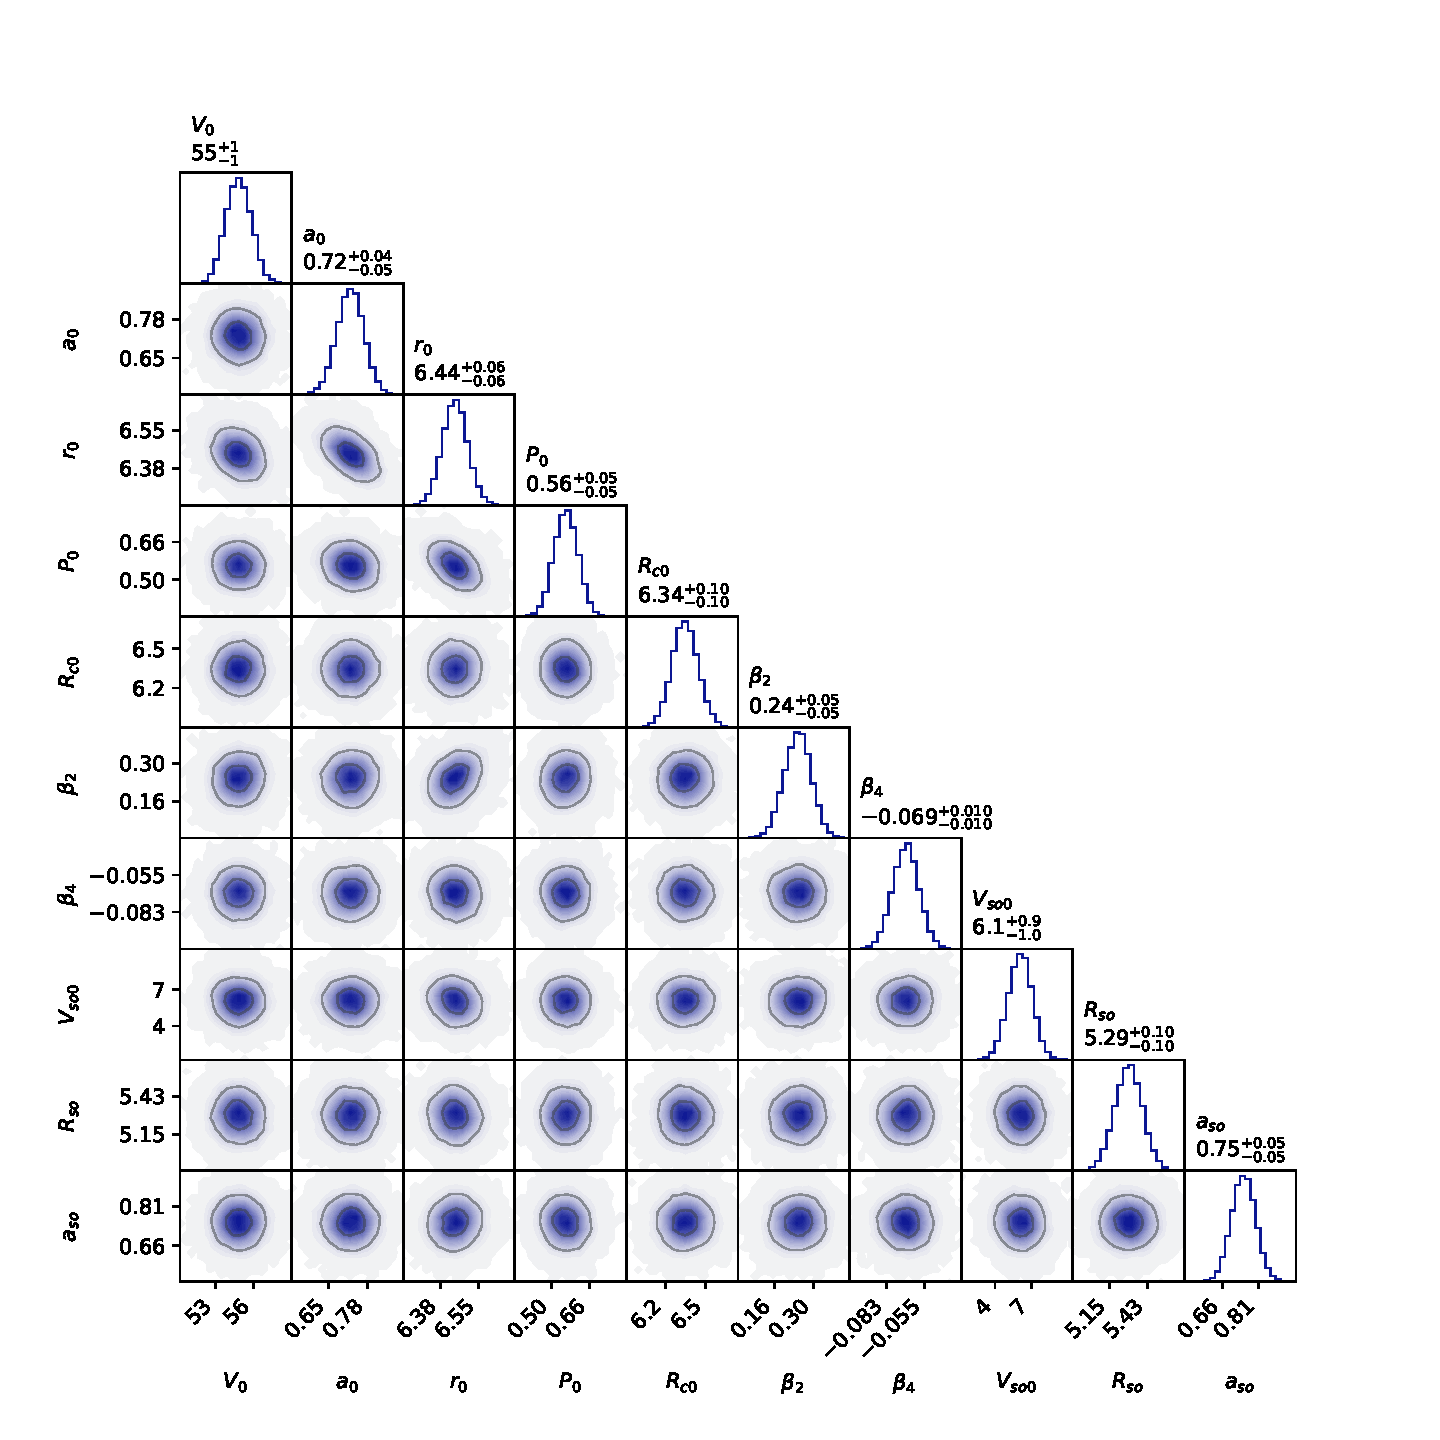
\includegraphics[width=0.8\textwidth]{Figures/figure1.pdf}
    \caption{Posterior distribution of the parameters for $^{145}Tm$ proton decay.}
    \label{fig:1}
\end{figure}

上图在helium1上计算,耗时约3.5d,速度较慢

后续预计先调整图片样式,然后做好代码优化加速,最后可以选取具体核区正式计算

我们使用如下代码修改样式: 
\begin{verbatim}
import prettyplease
from scipy.stats import norm
samples = sampler.get_chain(flat=True)

#a = v0,a0,r0,p0,rc0,beta2,beta4,vso0,rso,aso

labels = ["$V_0$", "$a_0$", "$r_0$", "$P_0$", "$R_{c0}$",
 "$\\beta_2$", "$\\beta_4$", "$V_{so0}$", "$R_{so}$", "$a_{so}$"]
fig, axes = prettyplease.corner(       
    samples,    
    labels=labels,
    bins=20,                         
    colors=['white', '#333333'],         
    linewidth=1.0,
    fontsize=10,
    n_ticks=3,
    return_axes=True
)

# ---------- 添加 1σ 区间竖线 ----------
ndim = samples.shape[1]       # 参数个数

# 先验参数定义（与 log_prior 保持一致）
prior_means = np.array([55, 0.75, 6.556, 0.580, 6.342, 0.231, -0.068, 6.2, 5.294, 0.75])
prior_sigmas = np.array([1, 0.05, 0.1, 0.05, 0.1, 0.05, 0.01, 1, 0.1, 0.05])

for i in range(ndim):
    ax = axes[i, i]           # 对角线子图
    data = samples[:, i]
    
    # 计算 16% 和 84% 分位数（对应 1σ 区间边界）
    q16, q84 = np.percentile(data, [16, 84])
    
    # 绘制两条虚线竖线
    ax.axvline(q16, color='red', linestyle='--', linewidth=1.0, alpha=0.8)
    ax.axvline(q84, color='red', linestyle='--', linewidth=1.0, alpha=0.8)
    median = np.median(data)
    ax.axvline(median, color='blue', linestyle='--', linewidth=1.0, alpha=0.8)

# ---------- 叠加先验曲线 ----------
for i in range(ndim):
    ax = axes[i, i]
    xlim = ax.get_xlim()
    x_plot = np.linspace(xlim[0], xlim[1], 200)
    pdf = norm.pdf(x_plot, loc=prior_means[i], scale=prior_sigmas[i])
    ax.plot(x_plot, pdf, color='green', linestyle='--', linewidth=1.2, alpha=0.8)
    ax.set_xlim(xlim)  # 恢复原范围



# plt.savefig('145Tm.pdf') 
plt.savefig('test.pdf')
plt.show() 
\end{verbatim}

示例图为

\begin{figure}[htbp]
    \centering
    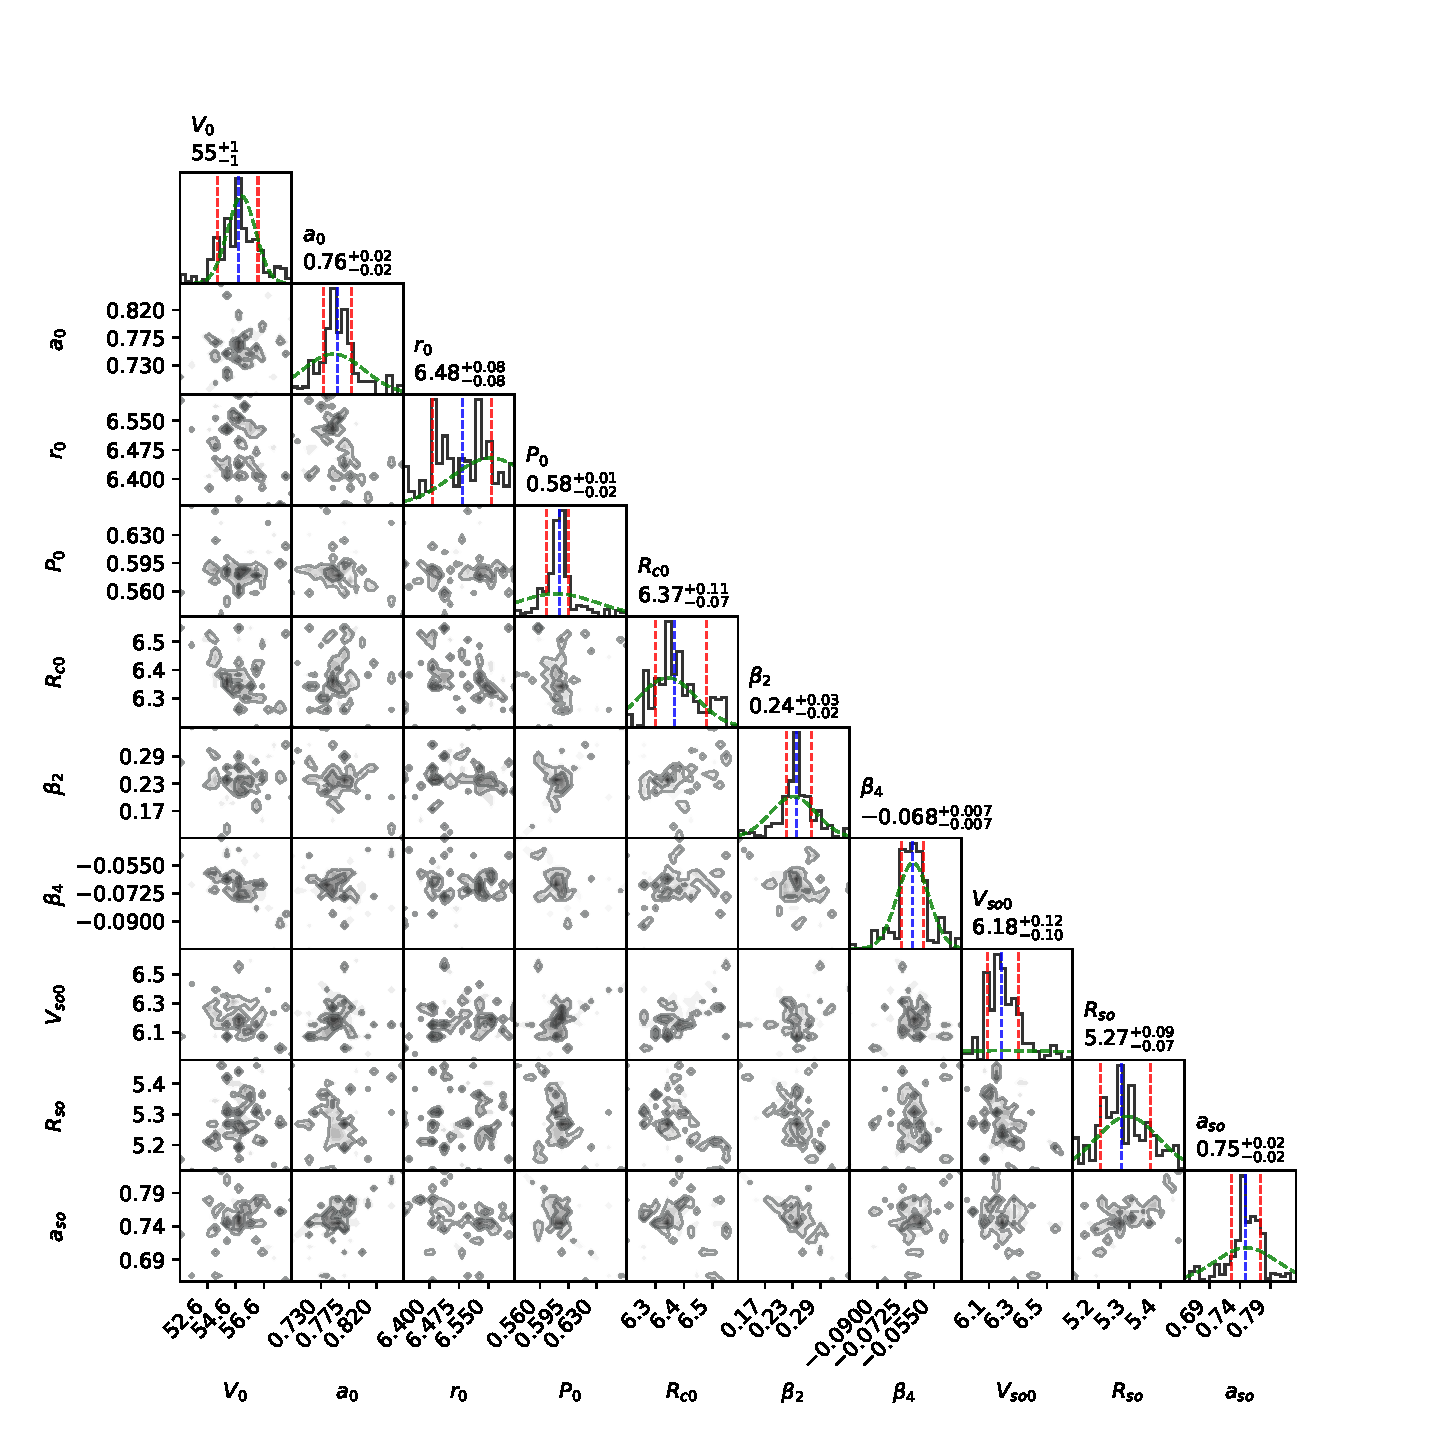
\includegraphics[width=0.8\textwidth]{Figures/figure2.pdf}
    \caption{后续计算使用的后验图的示例，包括增加了prior线，以及$1\sigma$，$2\sigma$，median的标定，还使用了灰色线图}
    \label{fig:2}
\end{figure}

对代码进行了部分优化后,显著提高了效率,在helium1上使用jupyter notebook运行, 使用参数如下
\begin{verbatim}
#System
e2=1.43997 ; hbarc=197.3269718 ; amu=931.49432
zp=69 ; Ap=145 ; mass_excess_p=-27.58 ; mp=Ap*amu+mass_excess_p
z1=68 ; A1=144 ; mass_excess_1=-36.61 ; m1=A1*amu+mass_excess_1    #1-> daughter
z2=1  ; A2=1   ; mass_excess_2=7.288971064 ; m2=A2*amu+mass_excess_2
Q=mp-m1-m2
mu=m1*m2/(m1+m2)
P0=0.580
#Potential

#Deformation
beta2 = 0.231  # quadrupole
beta4 = -0.068  # hexadecapole 

#Polarizaton
beta2tilde = 0  
beta4tilde = 0

#spin-orbit
Vso0=6.2 ; rso=1.01*(A1)**(1/3) ; aso=0.75 ; lambda_pi=np.sqrt(2)
L=5; S=0.5; J=5.5

#Vn
a0=0.75 ; r0=1.27*A1**(1/3)-0.1 ; V0=55

#Vc
Rc0 = 1.21 * A1**(1/3)          

#mesh
r = np.linspace(0.03, 30.0, 1000) # avoid too small r

# cached meshes for repeated gamma evaluations
ROOT_SEARCH_GRID = np.linspace(0.1, 100.0, 200)
R_GRID = np.linspace(0.05, 100.0, 600)
V_CENT_GRID = hbarc**2 * (L + 0.5)**2 / (2 * mu * R_GRID**2)
VC_THETA_GRID = np.linspace(0, np.pi / 2, 100)
VC_SIN_THETA = np.sin(VC_THETA_GRID)
VC_YL0_THETA = {
    lam: sph_harm_y(lam, 0, VC_THETA_GRID, 0).real for lam in (0, 2, 4)
}
VC_YL0_SIN_THETA = {
    lam: VC_YL0_THETA[lam] * VC_SIN_THETA for lam in (0, 2, 4)
}
Y00 = float(sph_harm_y(0, 0, 0.0, 0).real)
ASSAULT_QUAD_POINTS = 64
ACTION_QUAD_POINTS = 64
ROOT_XTOL = 1e-6
ROOT_ATOL = 1e-5    

# experiment data
y=np.array([3.16e-6])    # s
sigma=np.array([0.16e-6])

#a = v0,a0,r0,p0,rc0,beta2,beta4,vso0,rso,aso
def log_prior(a):
    v0,a0,r0,p0,rc0,beta2,beta4,vso0,rso,aso=a
    R=1
    
# Hyperparameters
    v0_mean=55; a0_mean=0.75; r0_mean=6.556; p0_mean=0.580
    rc0_mean=6.342; beta2_mean=0.231; beta4_mean=-0.068
    vso0_mean=6.2; rso_mean=5.294; aso_mean=0.75
    
    sigma_v0=1*R; sigma_a0=0.05*R; sigma_r0=0.1*R; sigma_p0=0.05*R
    sigma_rc0=0.1*R; sigma_beta2=0.05*R; sigma_beta4=0.01*R
    sigma_vso0=1*R; sigma_rso=0.1*R; sigma_aso=0.05*R

    
with multiprocessing.Pool() as pool:
    sampler = emcee.EnsembleSampler(nwalkers, M, log_posterior, 
    args=[y,sigma],a=1.0,pool=pool)
    state = sampler.run_mcmc(initial_positions, 200)
    sampler.reset()
    sampler.run_mcmc(state,5000)
\end{verbatim}
采样时间(不算画图和计算sigma区间的时间)约为25min
获得145Tm的后验图如下(5000/sampler的试运行)

\begin{figure}[htbp]
    \centering
    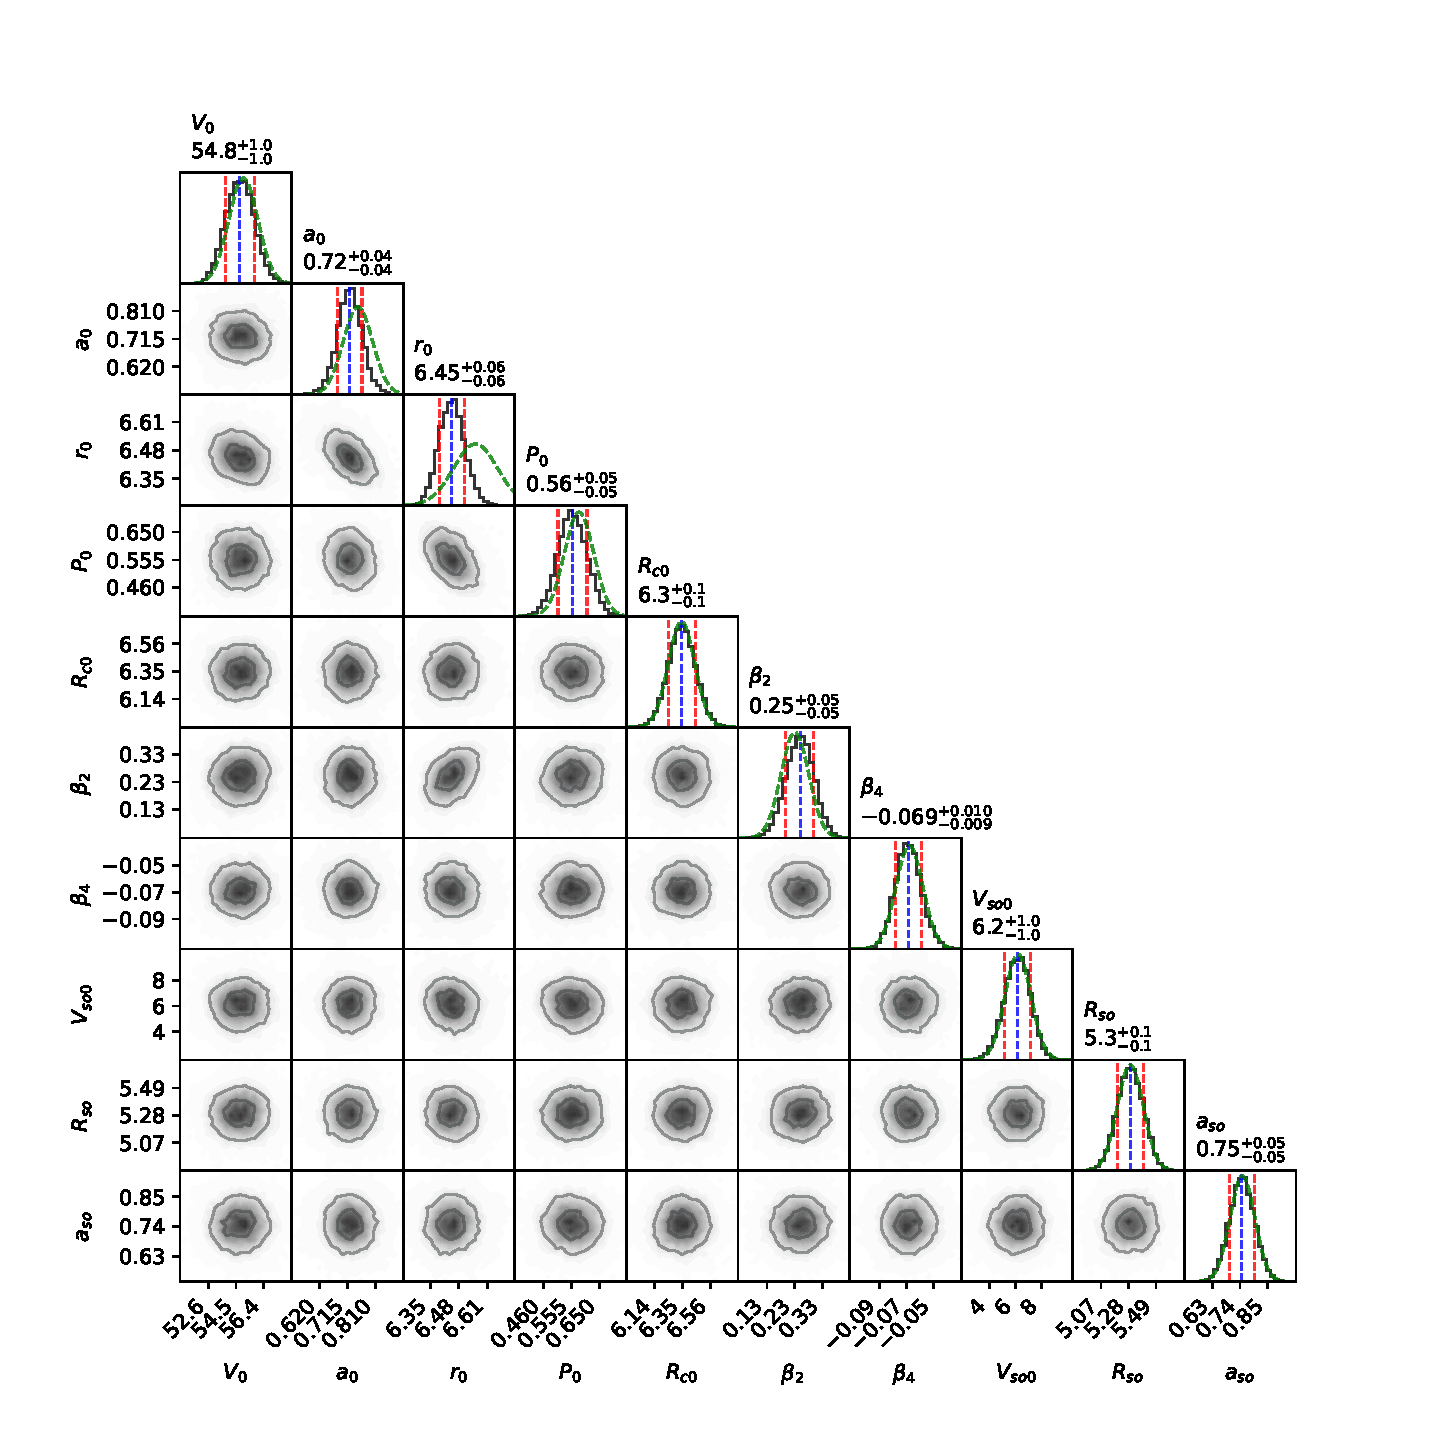
\includegraphics[width=0.8\textwidth]{Figures/figure3.pdf}
    \caption{145Tm的后验图(5000/sampler的试运行)}
    \label{fig:3}
\end{figure}
\clearpage
以及对应的confidence interval:
\begin{verbatim}
========== Posterior Predictive Distribution of Lifetime ==========
Number of posterior samples used: 5000
Mean lifetime      : 3.114e-06 s
Median lifetime    : 3.111e-06 s
Standard deviation : 1.568e-07 s
1σ error bar (±)   : 1.568e-07 s
2σ error bar (±)   : 3.137e-07 s
68% CI (1σ)        : [2.965e-06, 3.268e-06] s
95% CI (2σ)        : [2.811e-06, 3.429e-06] s
===================================================================    
\end{verbatim}
实验值在confidence interval内,说明模型的解释性没问题,代码运行也没问题

计算范式逻辑，除了可观测量的sigma区间，还包括了敏感性定量描述图，以及关联矩阵。示例图如下：

\begin{figure}[htbp]
    \centering
    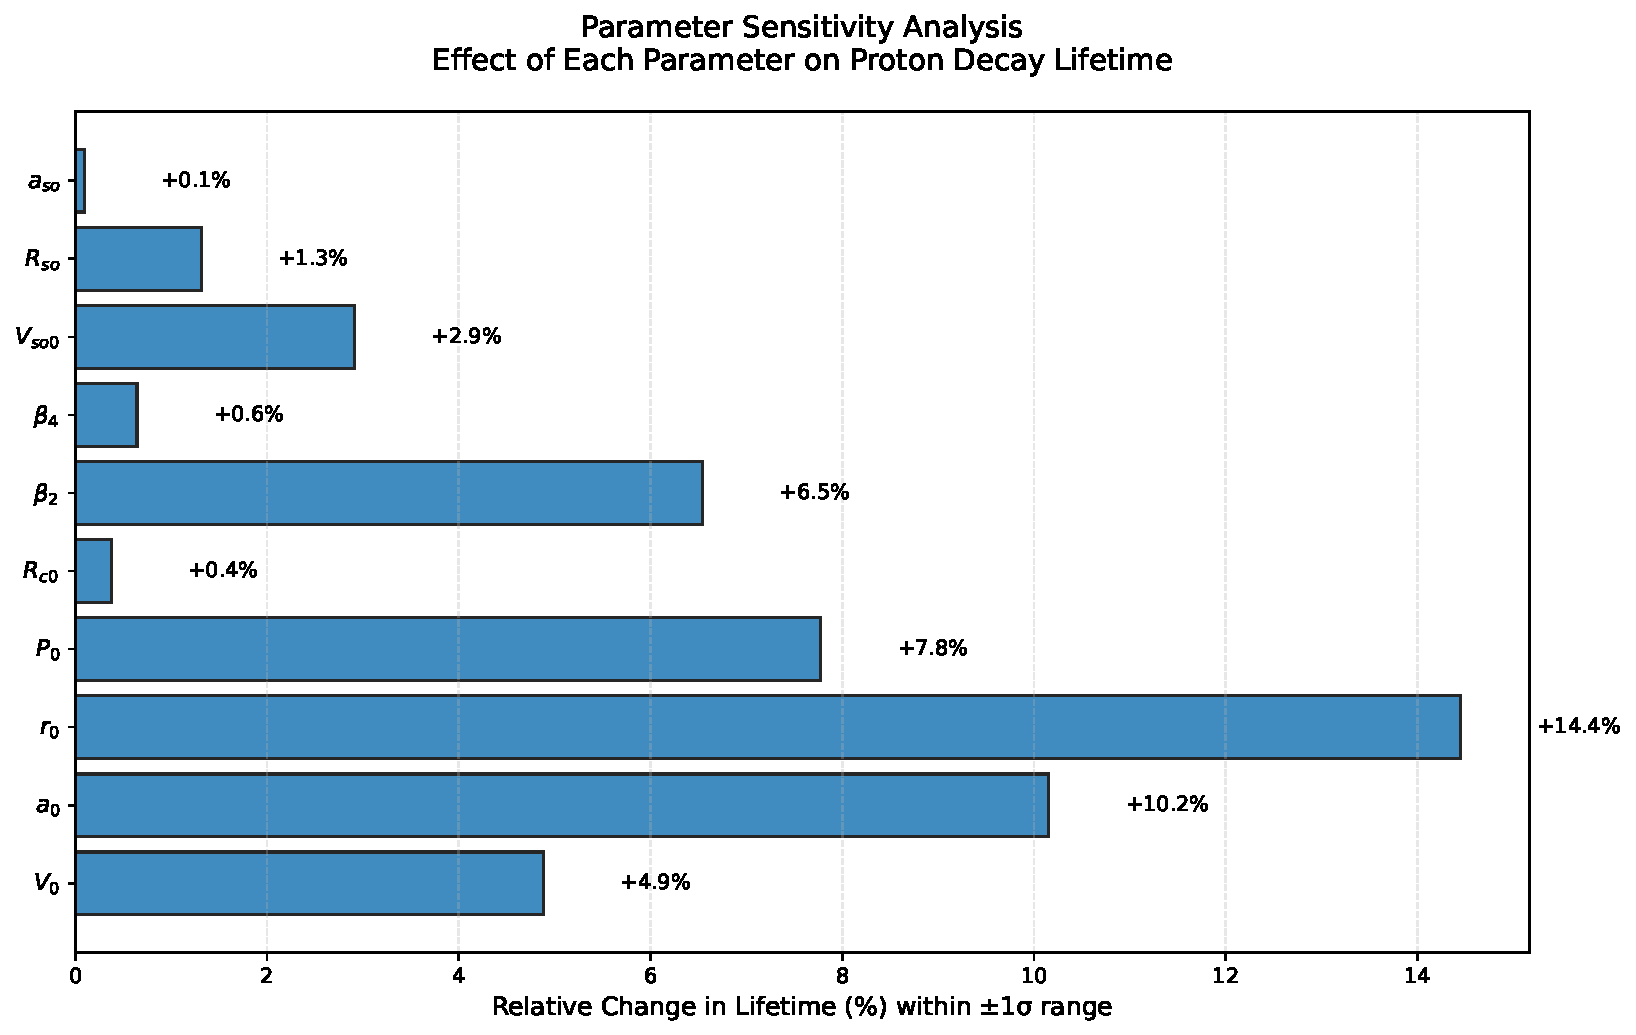
\includegraphics[width=0.8\textwidth]{Figures/figure4.pdf}
    \caption{参数敏感性图，横轴为参数，纵轴为对应参数的敏感性指标，红色竖线为实验值，蓝色竖线为模型预测值，灰色区域为模型预测的sigma区间。}
    \label{fig:4}
\end{figure}


\begin{figure}[htbp]
    \centering
    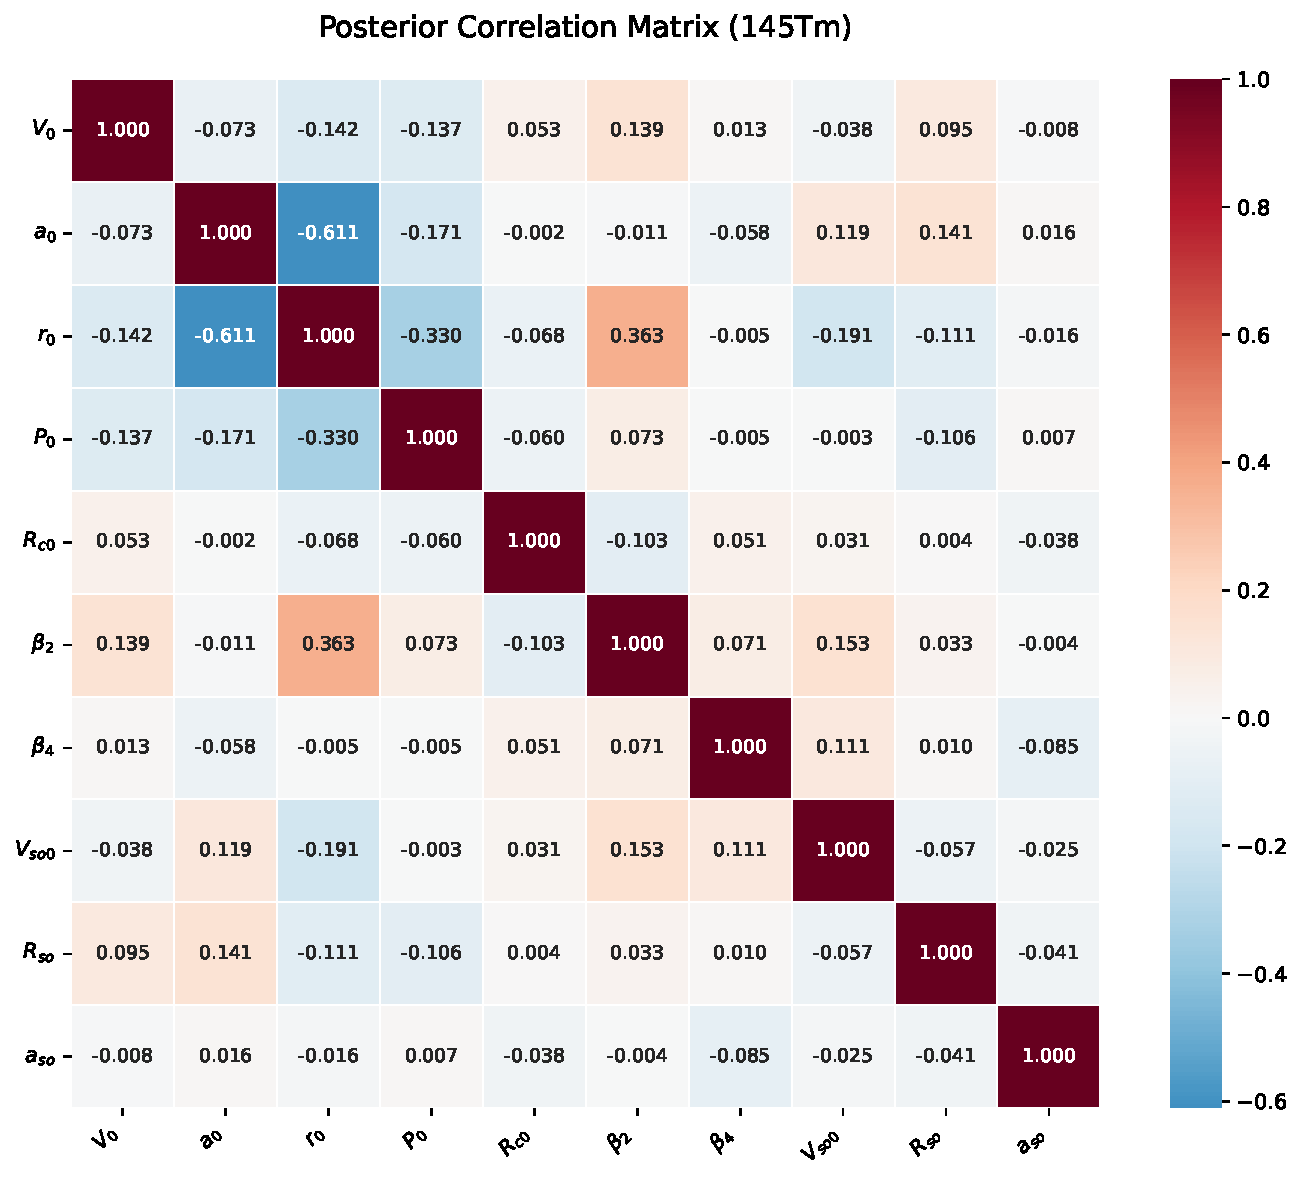
\includegraphics[width=0.8\textwidth]{Figures/figure5.pdf}
    \caption{关联矩阵}
    \label{fig:5}
\end{figure}
（上图使用了pandas和seaborn两个python包）
\clearpage

\section{正式运行}
这里打算研究远离质子幻数的区域，考虑质子幻数在50-82之间的质子衰变的核素（大部分选取了odd-odd或odd-A核）

{\color{blue}
从145Tm开始,进行正式运行,对145Tm选取计算参数
}

\begin{verbatim}
#System
e2=1.43997 ; hbarc=197.3269718 ; amu=931.49432
zp=69 ; Ap=145 ; mass_excess_p=-27.58 ; mp=Ap*amu+mass_excess_p
z1=68 ; A1=144 ; mass_excess_1=-36.61 ; m1=A1*amu+mass_excess_1    #1-> daughter
z2=1  ; A2=1   ; mass_excess_2=7.288971064 ; m2=A2*amu+mass_excess_2
Q=mp-m1-m2
mu=m1*m2/(m1+m2)
P0=0.580
#Potential

#Deformation
beta2 = 0.231  # quadrupole
beta4 = -0.068  # hexadecapole 

#Polarizaton
beta2tilde = 0  
beta4tilde = 0

#spin-orbit
Vso0=6.2 ; rso=1.01*(A1)**(1/3) ; aso=0.75 ; lambda_pi=np.sqrt(2)
L=5; S=0.5; J=5.5

#Vn
a0=0.75 ; r0=1.27*A1**(1/3)-0.1 ; V0=55

#Vc
Rc0 = 1.21 * A1**(1/3)          

#mesh
r = np.linspace(0.03, 30.0, 1000) # avoid too small r

# cached meshes for repeated gamma evaluations
ROOT_SEARCH_GRID = np.linspace(0.1, 100.0, 200)
R_GRID = np.linspace(0.05, 100.0, 600)
V_CENT_GRID = hbarc**2 * (L + 0.5)**2 / (2 * mu * R_GRID**2)
VC_THETA_GRID = np.linspace(0, np.pi / 2, 100)
VC_SIN_THETA = np.sin(VC_THETA_GRID)
VC_YL0_THETA = {
    lam: sph_harm_y(lam, 0, VC_THETA_GRID, 0).real for lam in (0, 2, 4)
}
VC_YL0_SIN_THETA = {
    lam: VC_YL0_THETA[lam] * VC_SIN_THETA for lam in (0, 2, 4)
}
Y00 = float(sph_harm_y(0, 0, 0.0, 0).real)
ASSAULT_QUAD_POINTS = 64
ACTION_QUAD_POINTS = 64
ROOT_XTOL = 1e-6
ROOT_ATOL = 1e-5

# experiment data
y=np.array([3.16e-6])    # s
sigma=np.array([0.16e-6])

#a = v0,a0,r0,p0,rc0,beta2,beta4,vso0,rso,aso
def log_prior(a):
    v0,a0,r0,p0,rc0,beta2,beta4,vso0,rso,aso=a
    R=1
    
# Hyperparameters
    v0_mean=55; a0_mean=0.75; r0_mean=6.556; p0_mean=0.580
    rc0_mean=6.342; beta2_mean=0.231; beta4_mean=-0.068
    vso0_mean=6.2; rso_mean=5.294; aso_mean=0.75
    
    sigma_v0=1*R; sigma_a0=0.05*R; sigma_r0=0.1*R; sigma_p0=0.05*R
    sigma_rc0=0.1*R; sigma_beta2=0.05*R; sigma_beta4=0.01*R
    sigma_vso0=1*R; sigma_rso=0.1*R; sigma_aso=0.05*R

with multiprocessing.Pool() as pool:
    sampler = emcee.EnsembleSampler(nwalkers, M, log_posterior, 
    args=[y,sigma],a=2.0,pool=pool)
    state = sampler.run_mcmc(initial_positions, 200)
    sampler.reset()
    sampler.run_mcmc(state,5000)
\end{verbatim}

得到的posterior图

\begin{figure}[htbp]
    \centering
    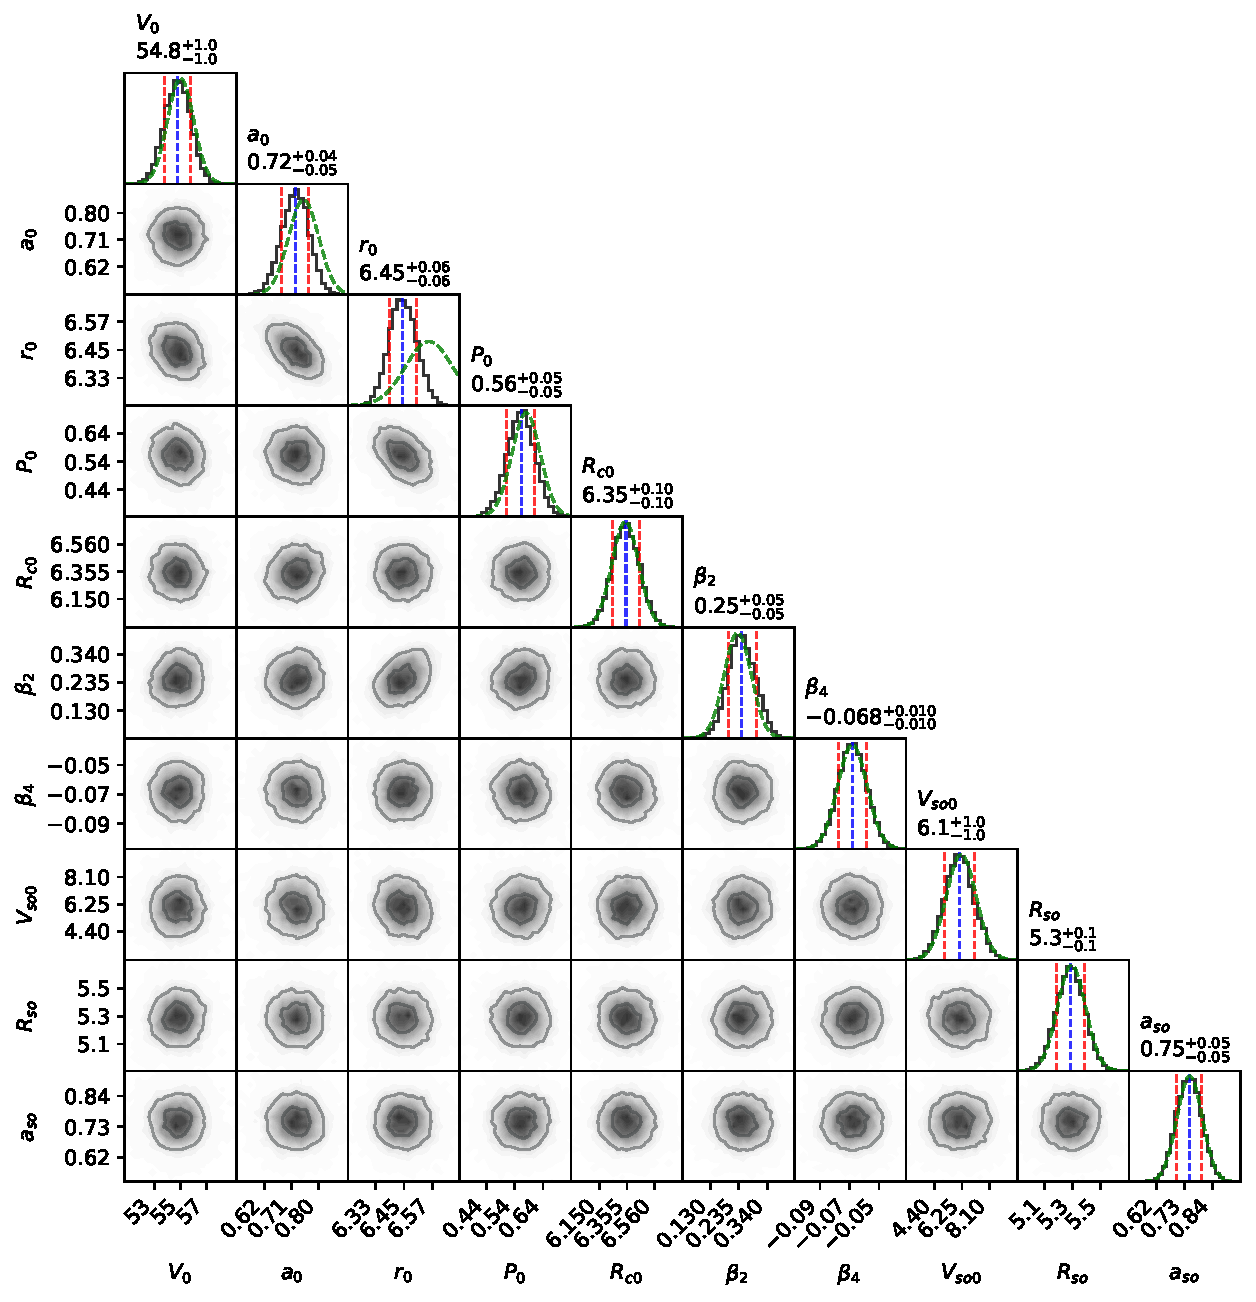
\includegraphics[width=0.8\textwidth]{Figures/figure6.pdf}
    \caption{145Tm的后验图(5000samples/sampler的正式运行)}
    \label{fig:6}
\end{figure}

其参数敏感性分析如下
\begin{figure}[htbp]
    \centering
    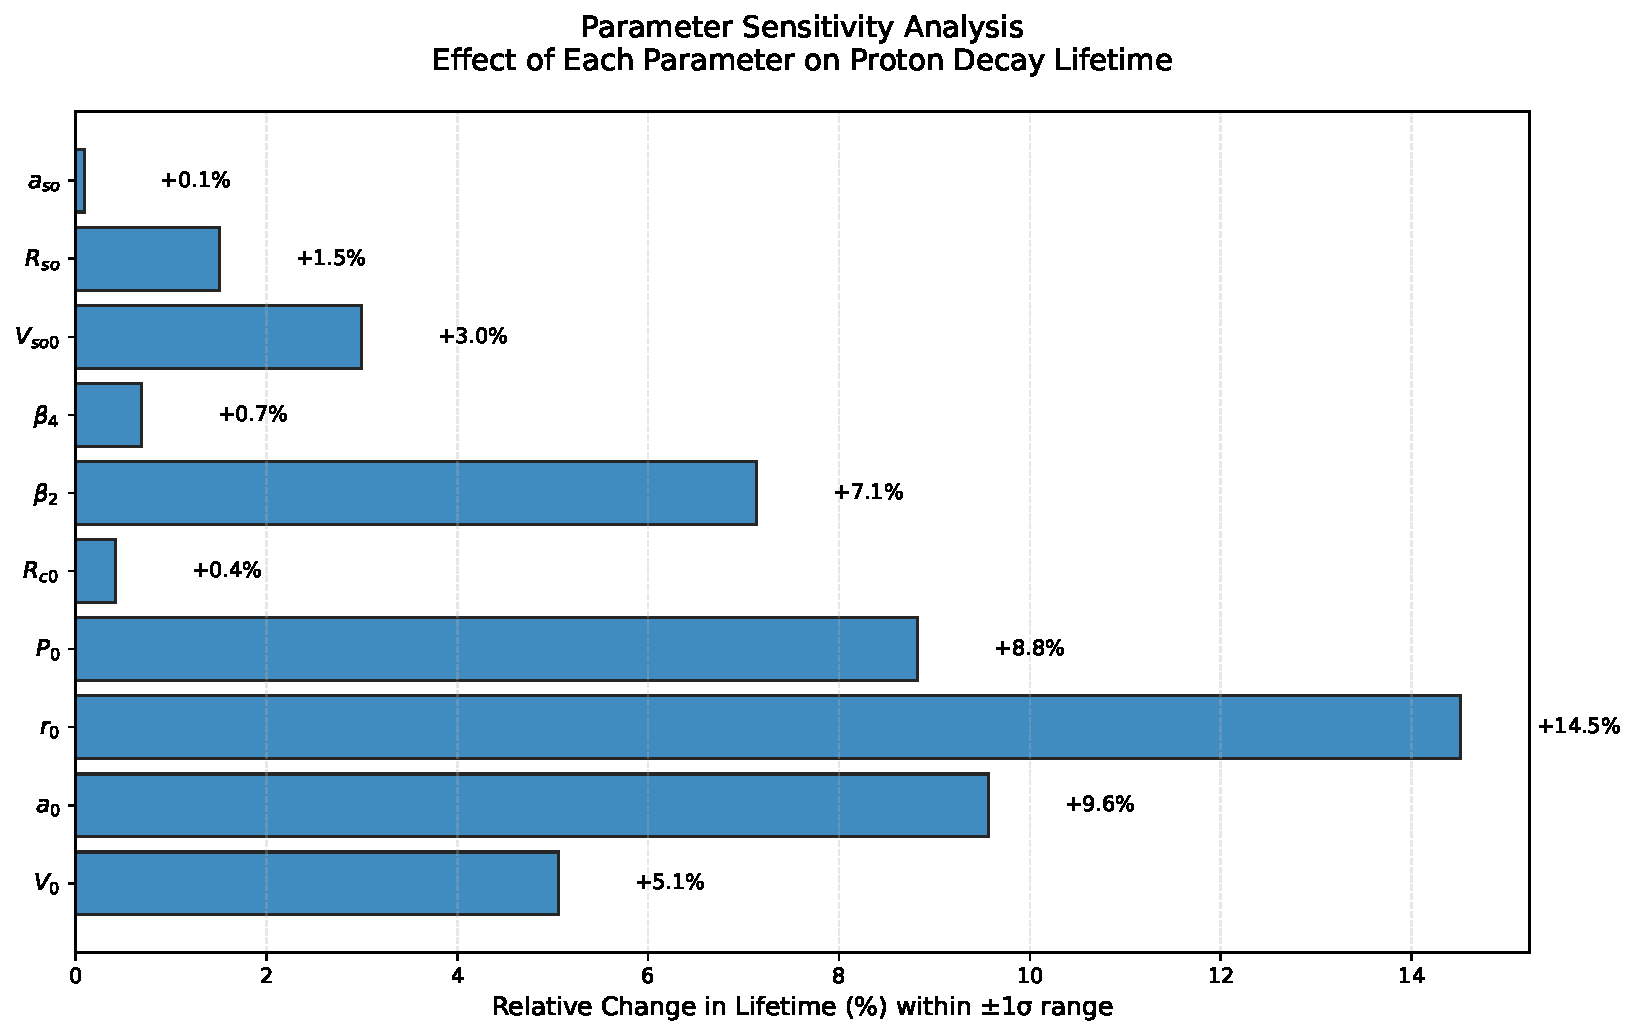
\includegraphics[width=0.8\textwidth]{Figures/figure7.pdf}
    \caption{145Tm的参数敏感性图(1sigma区间内的参数变化对半衰期的影响)}
    \label{fig:7}
\end{figure}


参数关联图如下

\begin{figure}[htbp]
    \centering
    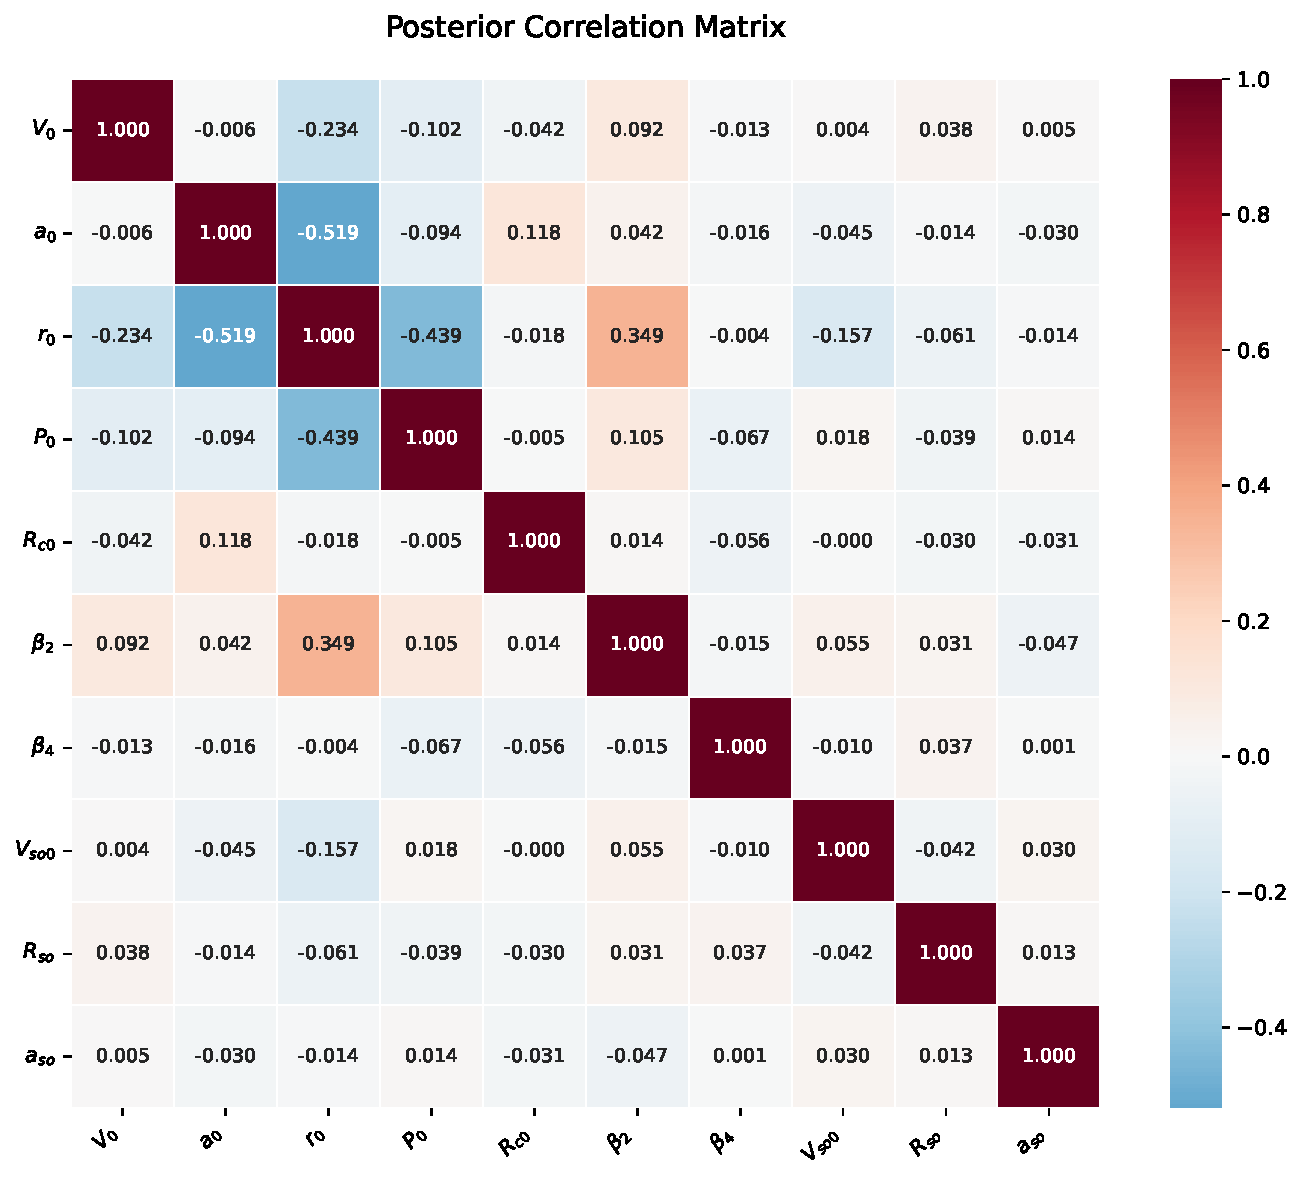
\includegraphics[width=0.8\textwidth]{Figures/figure8.pdf}
    \caption{145Tm的形变势能参数的关联矩阵}
    \label{fig:8}
\end{figure}
\clearpage

145Tm可观测量的sigma区间如下(为计算方便，从很多samples中间均匀抽取5000个进行计算)
\begin{verbatim}
========== Posterior Predictive Distribution of Lifetime ==========
Experiment data: 3.16e-6 s
Number of posterior samples used: 5000
Mean lifetime      : 3.109e-06 s
Median lifetime    : 3.109e-06 s
Standard deviation : 1.624e-07 s
1σ error bar (±)   : 1.624e-07 s
2σ error bar (±)   : 3.248e-07 s
68% CI (1σ)        : [2.945e-06, 3.274e-06] s
95% CI (2σ)        : [2.797e-06, 3.424e-06] s
===================================================================
\end{verbatim}

{\color{blue}
然后对109I进行研究
}

对于109I这个核素，选取计算参数如下：
\begin{verbatim}
#System of Proton Decay
e2=1.43997 ; hbarc=197.3269718 ; amu=931.49432
zp=53 ; Ap=109 ; mass_excess_p=-57.673 ; mp=Ap*amu+mass_excess_p        #Parent
z1=zp-1 ; A1=Ap-1 ; mass_excess_1=-65.782 ; m1=A1*amu+mass_excess_1    #1-> daughter
z2=1  ; A2=1   ; mass_excess_2=7.288971064 ; m2=A2*amu+mass_excess_2
Q=mp-m1-m2
mu=m1*m2/(m1+m2)
P0=0.726
#Potential

#Deformation
beta2 = 0.139  # quadrupole
beta4 = 0.056  # hexadecapole 

#Polarizaton
beta2tilde = 0  
beta4tilde = 0

#spin-orbit
Vso0=6.2 ; rso=1.01*(A1)**(1/3) ; aso=0.75 ; lambda_pi=np.sqrt(2)
L=2; S=0.5; J=1.5
print("rso=",rso)
#Vn
a0=0.75 ; r0=1.27*A1**(1/3)-0.1 ; V0=55
print("r0=",r0)
#Vc
Rc0 = 1.21 * A1**(1/3)          
print("Rc0=",Rc0)
#mesh
r = np.linspace(0.03, 30.0, 1000) # avoid too small r

# experiment data
y=np.array([92.7e-6])    # s
sigma=np.array([0.7e-6])

# Hyperparameters
    v0_mean=55; a0_mean=0.75; r0_mean=5.948; p0_mean=0.726
    rc0_mean=5.762; beta2_mean=0.139; beta4_mean=0.056
    vso0_mean=6.2; rso_mean=4.809; aso_mean=0.75

with multiprocessing.Pool() as pool:
    sampler = emcee.EnsembleSampler(nwalkers, M, log_posterior, 
    args=[y,sigma],a=2.0,pool=pool)
    state = sampler.run_mcmc(initial_positions, 200)
    sampler.reset()
    sampler.run_mcmc(state,10000)
\end{verbatim}

获得了109I的posterior：
\begin{figure}[htbp]
    \centering
    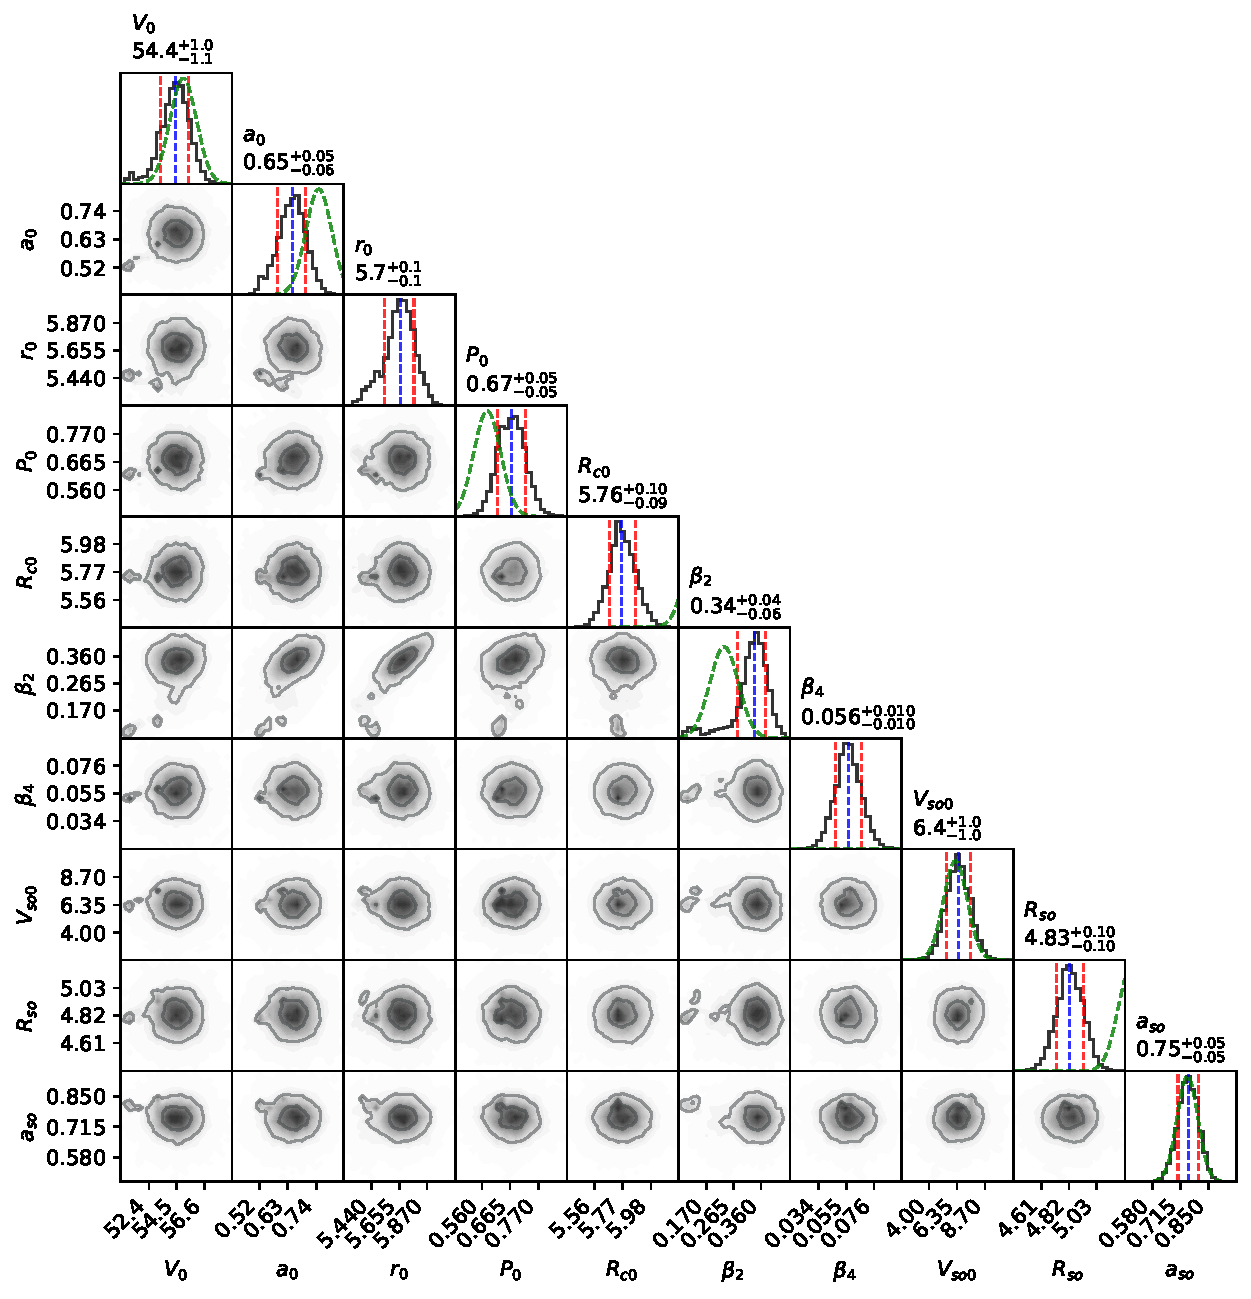
\includegraphics[width=0.8\textwidth]{Figures/figure9.pdf}
    \caption{109I的后验图(10000samples/sampler的正式运行)}
    \label{fig:9}
\end{figure}

然后是109I的参数敏感性图：
\begin{figure}[htbp]
    \centering
    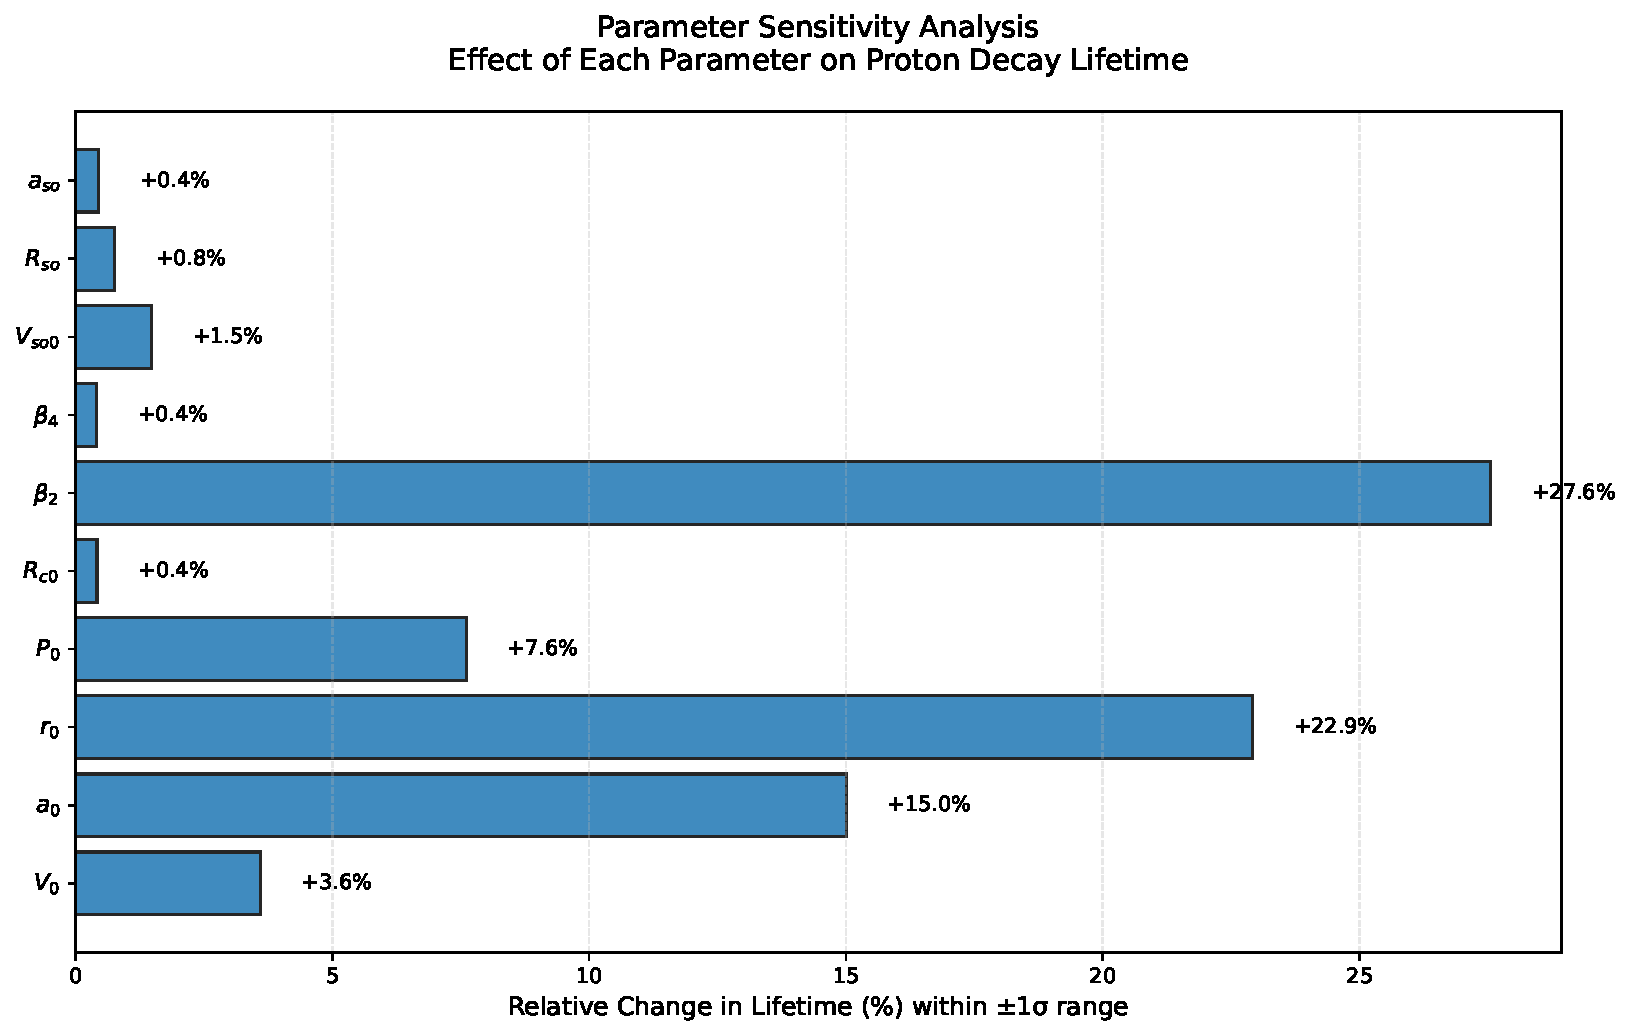
\includegraphics[width=0.8\textwidth]{Figures/figure10.pdf}
    \caption{109I的参数敏感性图(1sigma区间内的参数变化对半衰期的影响)}
    \label{fig:10}
\end{figure}

然后是109I的参数关联图：
\begin{figure}[htbp]
    \centering
    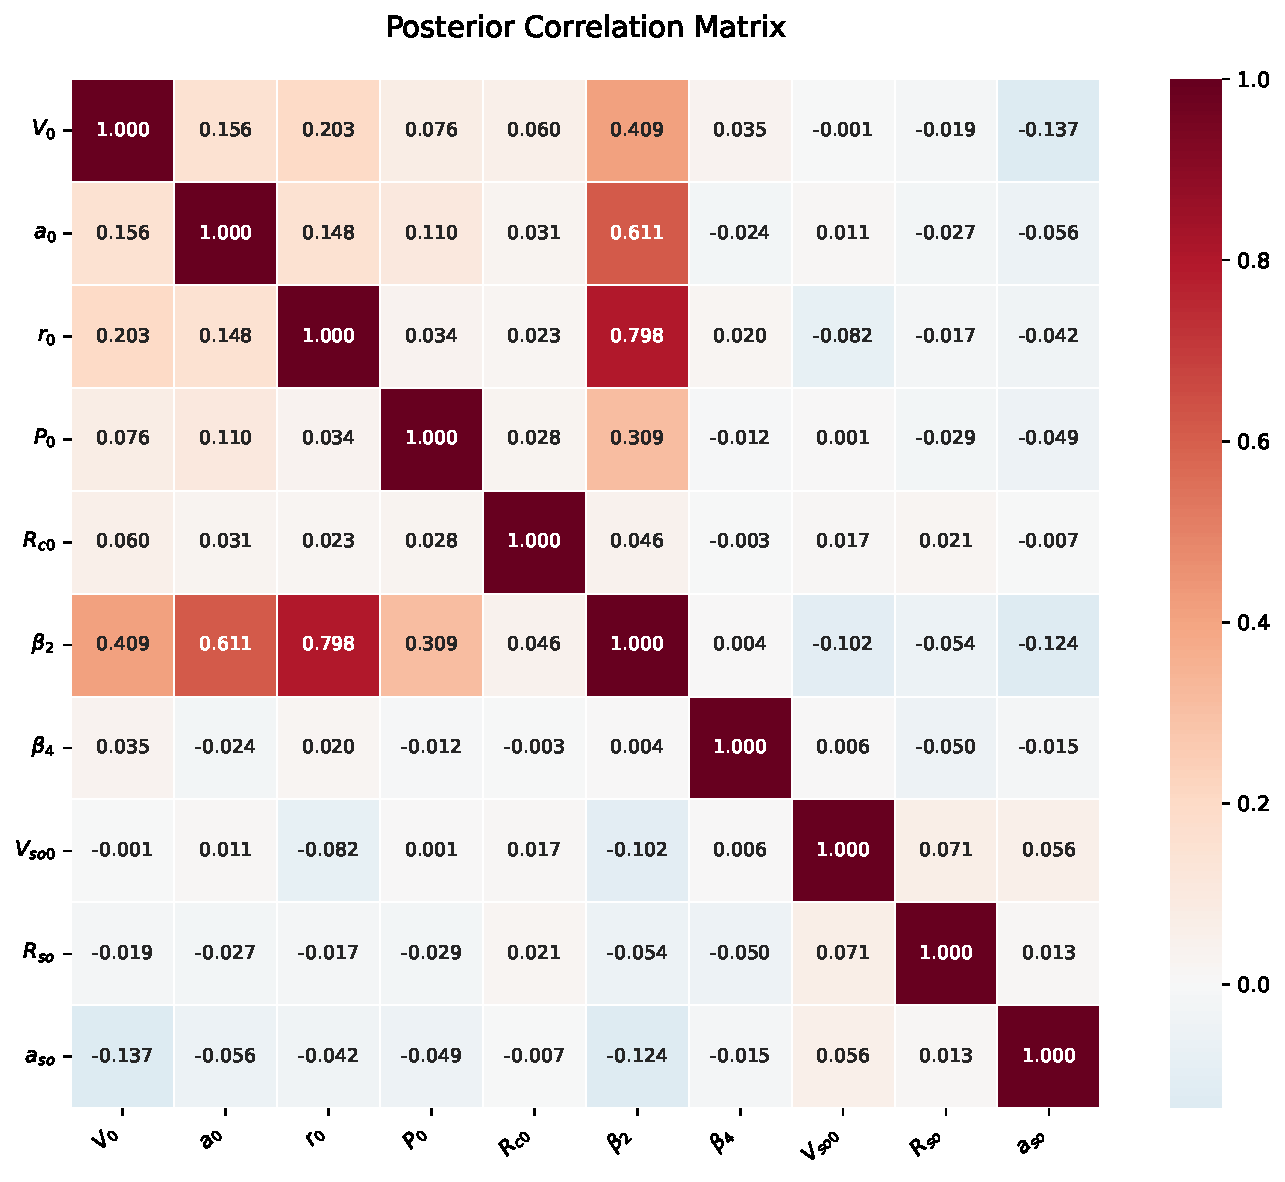
\includegraphics[width=0.8\textwidth]{Figures/figure11.pdf}
    \caption{109I的形变势能参数的关联矩阵}
    \label{fig:11}
\end{figure}

最后是109I的可观测量sigma区间：
\begin{verbatim}
========== Posterior Predictive Distribution of Lifetime ==========
experiment data: [9.27e-05] s
Number of posterior samples used: 5000
Mean lifetime      : 9.261e-05 s
Median lifetime    : 9.260e-05 s
Standard deviation : 7.155e-07 s
1σ error bar (±)   : 7.155e-07 s
2σ error bar (±)   : 1.431e-06 s
68% CI (1σ)        : [9.190e-05, 9.332e-05] s
95% CI (2σ)        : [9.120e-05, 9.403e-05] s
===================================================================
\end{verbatim}


\clearpage

然后是对113Cs的研究计算，对于113Cs选取了计算参数：
\begin{verbatim}
#System of Proton Decay
e2=1.43997 ; hbarc=197.3269718 ; amu=931.49432
zp=55 ; Ap=113 ; mass_excess_p=-51.765 ; mp=Ap*amu+mass_excess_p        #Parent
z1=zp-1 ; A1=Ap-1 ; mass_excess_1=-60.026 ; m1=A1*amu+mass_excess_1    #1-> daughter
z2=1  ; A2=1   ; mass_excess_2=7.288971064 ; m2=A2*amu+mass_excess_2
Q=mp-m1-m2
print("Q=",Q)
mu=m1*m2/(m1+m2)
P0=0.373
#Potential

#Deformation
beta2 = 0.195  # quadrupole
beta4 = 0.054  # hexadecapole 

#Polarizaton
beta2tilde = 0  
beta4tilde = 0

#spin-orbit
Vso0=6.2 ; rso=1.01*(A1)**(1/3) ; aso=0.75 ; lambda_pi=np.sqrt(2)
L=2; S=0.5; J=1.5
print("rso=",rso)
#Vn
a0=0.75 ; r0=1.27*A1**(1/3)-0.1 ; V0=55
print("r0=",r0)
#Vc
Rc0 = 1.21 * A1**(1/3)          
print("Rc0=",Rc0)
#mesh
r = np.linspace(0.03, 30.0, 1000) # avoid too small r   


# experiment data
y=np.array([16.9e-6])    # s
sigma=np.array([0.1e-6])

# Hyperparameters
    v0_mean=55; a0_mean=0.75; r0_mean=6.021; p0_mean=0.373
    rc0_mean=5.832; beta2_mean=0.195; beta4_mean=0.054
    vso0_mean=6.2; rso_mean=4.868; aso_mean=0.75


    sampler = emcee.EnsembleSampler(nwalkers, M, log_posterior, args=[y,sigma],
    a=2.0,pool=pool)
    state = sampler.run_mcmc(initial_positions, 500)
    sampler.reset()
    sampler.run_mcmc(state,10000)
\end{verbatim}
这里选择了默认值的采样参数$a=2.0$以及更多的burn-in steps 500。

获得的posterior

\begin{figure}[htbp]
    \centering
    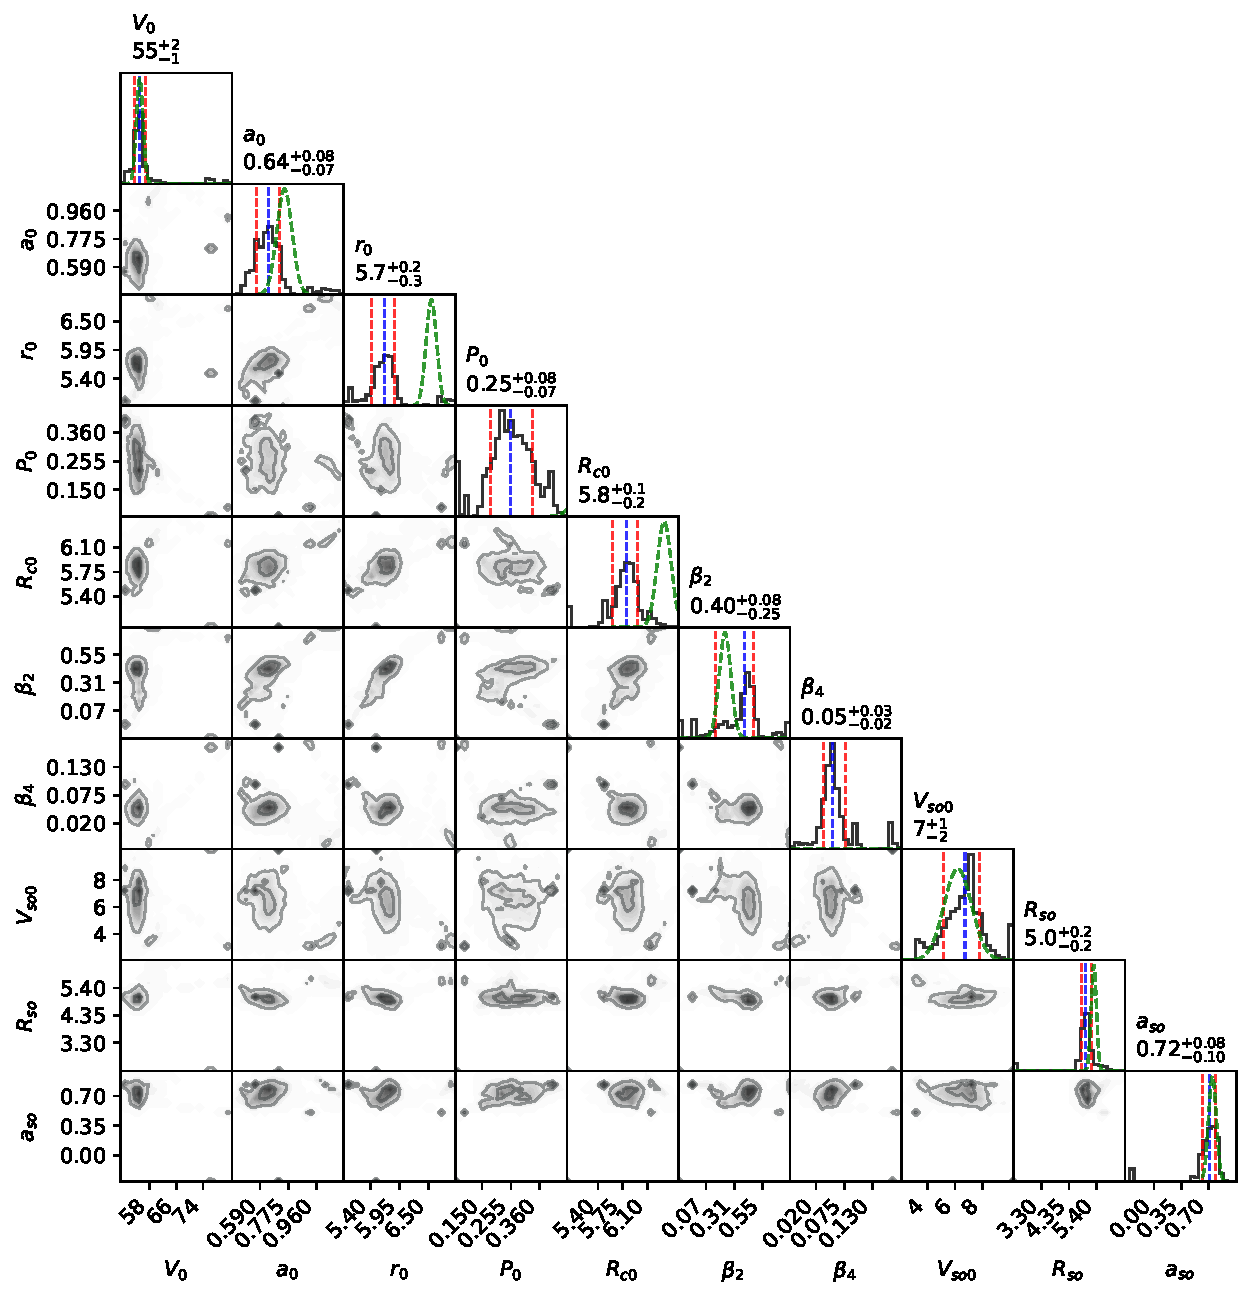
\includegraphics[width=0.8\textwidth]{Figures/figure12.pdf}
    \caption{113Cs的后验图(10000samples/sampler的正式运行,但burnin step为500)，这里获得了一定correlation}
    \label{fig:12}
\end{figure}

然后是113Cs的参数敏感性图：
\begin{figure}[htbp]
    \centering
    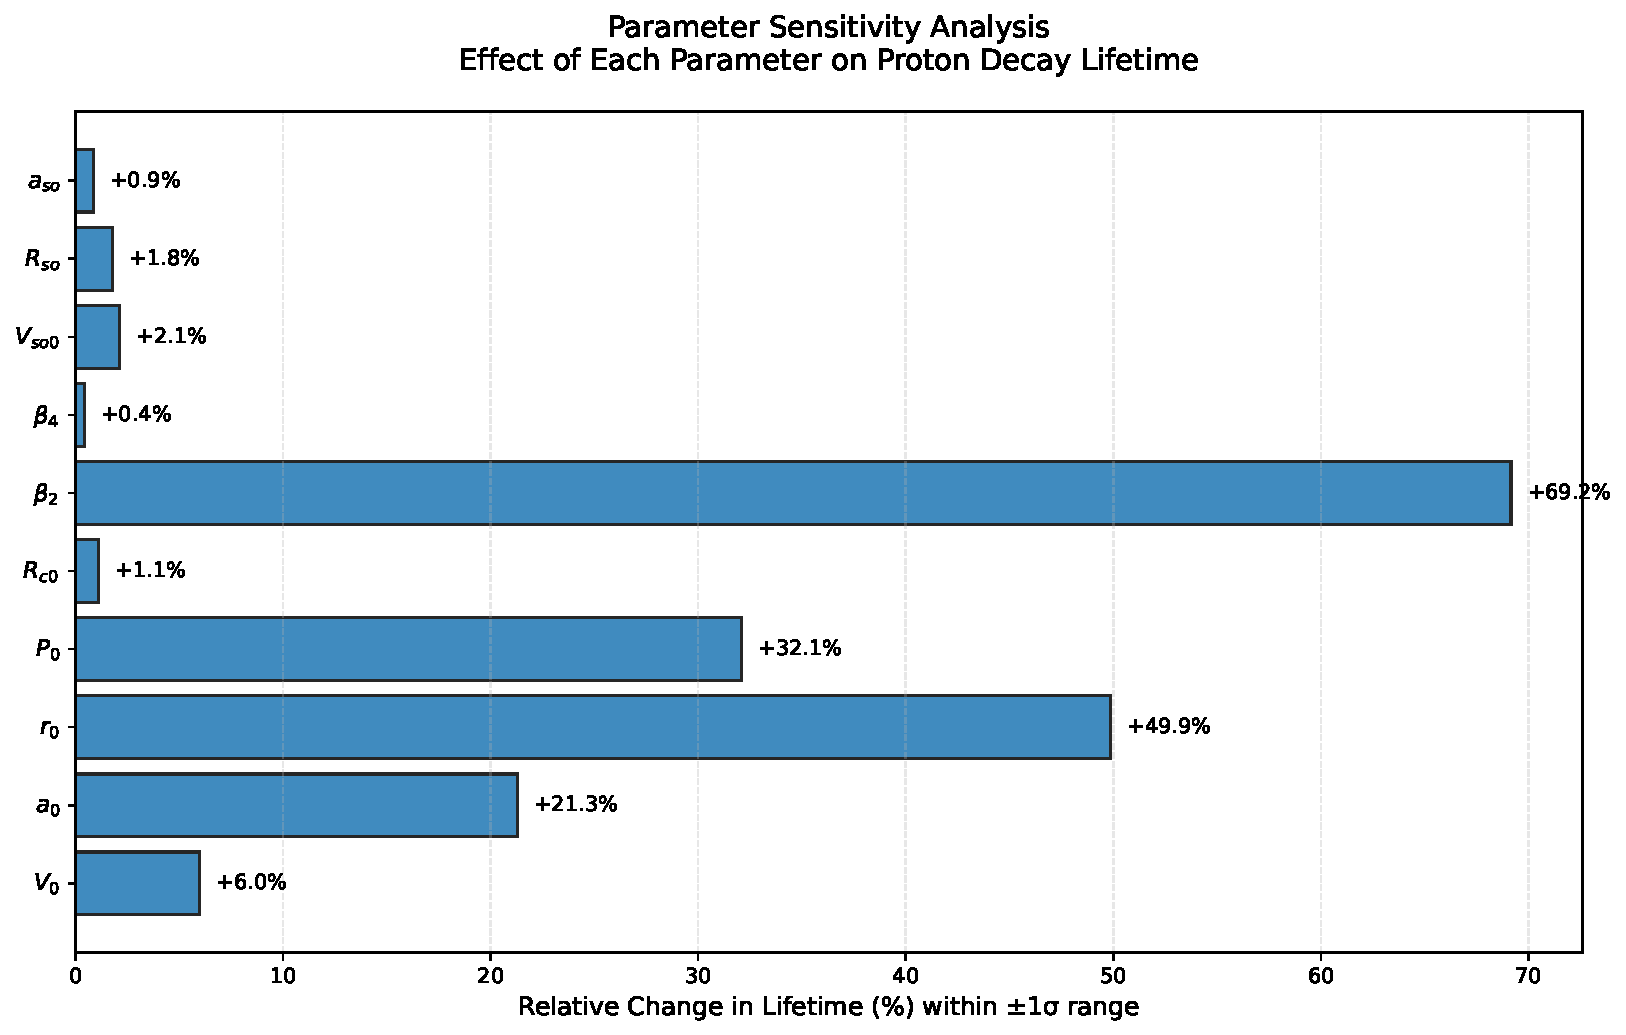
\includegraphics[width=0.8\textwidth]{Figures/figure13.pdf}
    \caption{113Cs的参数敏感性图(1sigma区间内的参数变化对半衰期的影响)}
    \label{fig:13}
\end{figure}

然后是113Cs的参数关联图：
\begin{figure}[htbp]
    \centering
    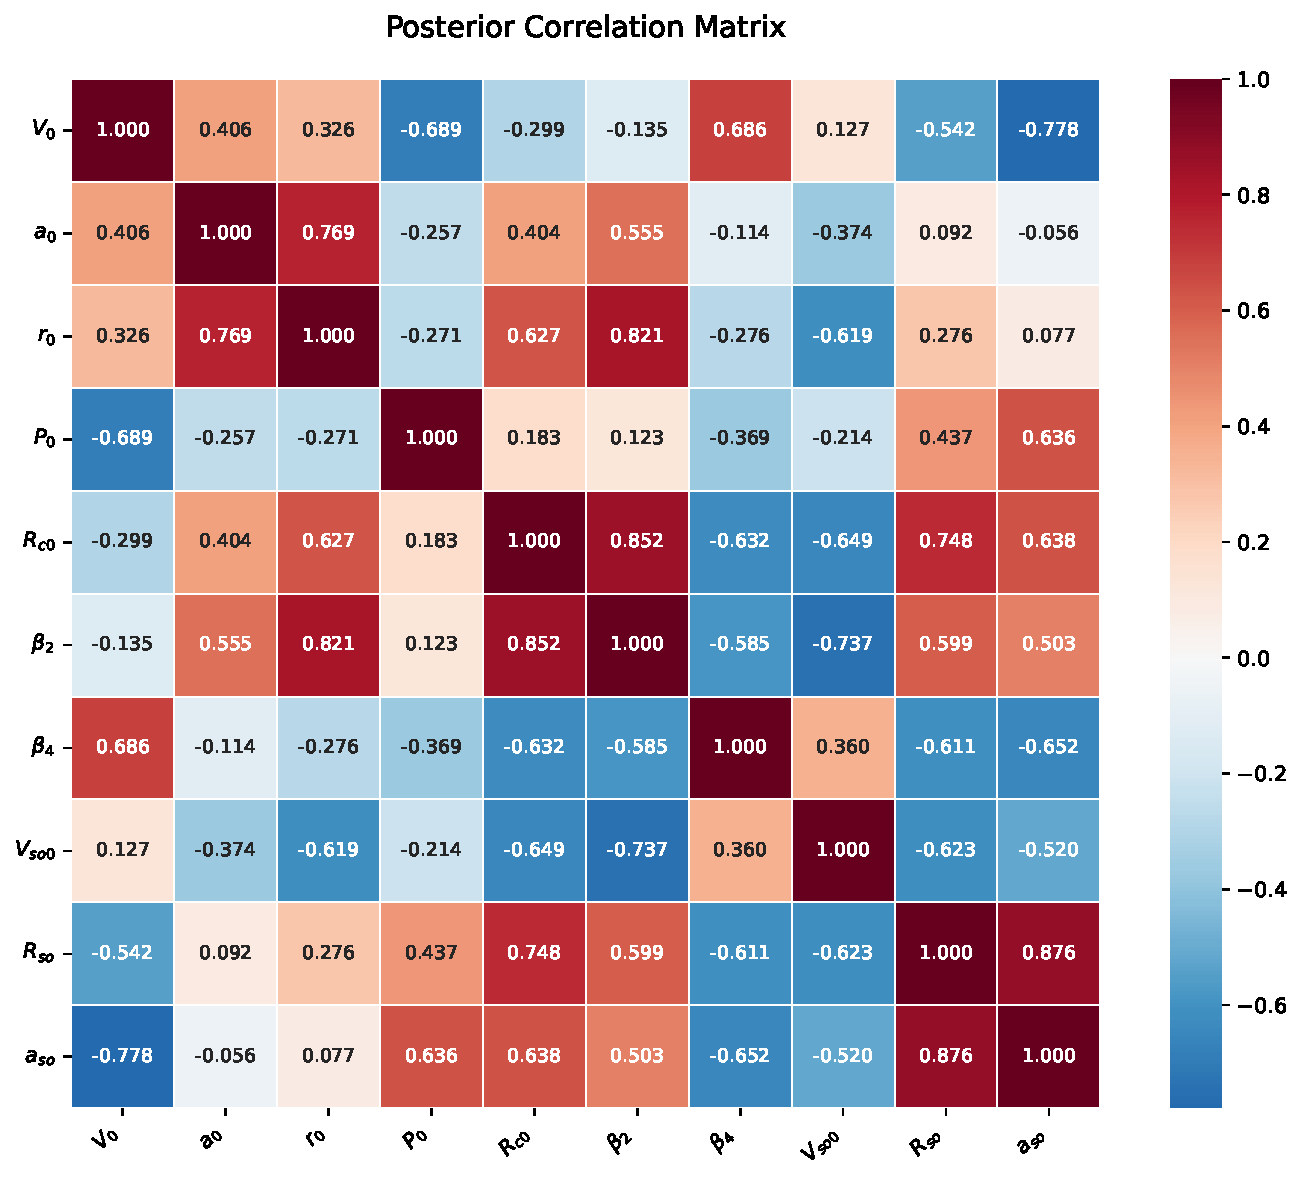
\includegraphics[width=0.8\textwidth]{Figures/figure14.pdf}
    \caption{113Cs的形变势能参数的关联矩阵,非对角项明显有一定值，体现了correlation}
    \label{fig:14}
\end{figure}

\clearpage
最后是sigma区间：
\begin{verbatim}
========== Posterior Predictive Distribution of Lifetime ==========
experiment data: [1.69e-05] s
Number of posterior samples used: 5000
Mean lifetime      : 1.685e-05 s
Median lifetime    : 1.687e-05 s
Standard deviation : 1.384e-07 s
1σ error bar (±)   : 1.384e-07 s
2σ error bar (±)   : 2.767e-07 s
68% CI (1σ)        : [1.673e-05, 1.698e-05] s
95% CI (2σ)        : [1.651e-05, 1.708e-05] s
===================================================================    
\end{verbatim}

然后我们对117La进行研究，选取计算参数如下：

\begin{verbatim}
#117La
e2=1.43997 ; hbarc=197.3269718 ; amu=931.49432
zp=57 ; Ap=117 ; mass_excess_p=-46.27 ; mp=Ap*amu+mass_excess_p        #Parent
z1=zp-1 ; A1=Ap-1 ; mass_excess_1=-54.38 ; m1=A1*amu+mass_excess_1    #1-> daughter
z2=1  ; A2=1   ; mass_excess_2=7.288971064 ; m2=A2*amu+mass_excess_2
Q=mp-m1-m2
print("Q=",Q)
mu=m1*m2/(m1+m2)
P0=0.311
#Potential

#Deformation
beta2 = 0.282  # quadrupole
beta4 = 0.106  # hexadecapole 

#Polarizaton
beta2tilde = 0  
beta4tilde = 0

#spin-orbit
Vso0=6.2 ; rso=1.01*(A1)**(1/3) ; aso=0.75 ; lambda_pi=np.sqrt(2)
L=2; S=0.5; J=1.5
print("rso=",rso)
#Vn
a0=0.75 ; r0=1.27*A1**(1/3)-0.1 ; V0=55
print("r0=",r0)
#Vc
Rc0 = 1.21 * A1**(1/3)          
print("Rc0=",Rc0)
#mesh
r = np.linspace(0.03, 30.0, 1000) # avoid too small r

# cached meshes for repeated gamma evaluations
ROOT_SEARCH_GRID = np.linspace(0.1, 150.0, 500)
R_GRID = np.linspace(0.05, 150.0, 600)
V_CENT_GRID = hbarc**2 * (L + 0.5)**2 / (2 * mu * R_GRID**2)
VC_THETA_GRID = np.linspace(0, np.pi / 2, 100)
VC_SIN_THETA = np.sin(VC_THETA_GRID)
VC_YL0_THETA = {
    lam: sph_harm_y(lam, 0, VC_THETA_GRID, 0).real for lam in (0, 2, 4)
}
VC_YL0_SIN_THETA = {
    lam: VC_YL0_THETA[lam] * VC_SIN_THETA for lam in (0, 2, 4)
}
Y00 = float(sph_harm_y(0, 0, 0.0, 0).real)
ASSAULT_QUAD_POINTS = 64
ACTION_QUAD_POINTS = 64
ROOT_XTOL = 1e-6
ROOT_ATOL = 1e-5



# experiment data
y=np.array([21.7e-3])    # s
sigma=np.array([1.8e-3])

# Hyperparameters in Prior
    v0_mean=55; a0_mean=0.75; r0_mean=1.27*A1**(1/3)-0.1; p0_mean=0.311
    rc0_mean=1.21 * A1**(1/3); beta2_mean=0.282; beta4_mean=0.106
    vso0_mean=6.2; rso_mean=1.01*(A1)**(1/3); aso_mean=0.75

with multiprocessing.Pool() as pool:
    sampler = emcee.EnsembleSampler(nwalkers, M, log_posterior, 
    args=[y,sigma],a=2.0,pool=pool)
    state = sampler.run_mcmc(initial_positions, 200)
    sampler.reset()
    sampler.run_mcmc(state,10000)

\end{verbatim}

这里增大了r的mesh范围，因为势能的范围变大了（之前的小范围r的mesh导致了根没有完全搜索完），
此外还将prior中的几个$r_0$相关的超参数直接写为和$A$相关的公式形式，这是一个方便的改动.

首先是posterior图：
\begin{figure}[htbp]
    \centering
    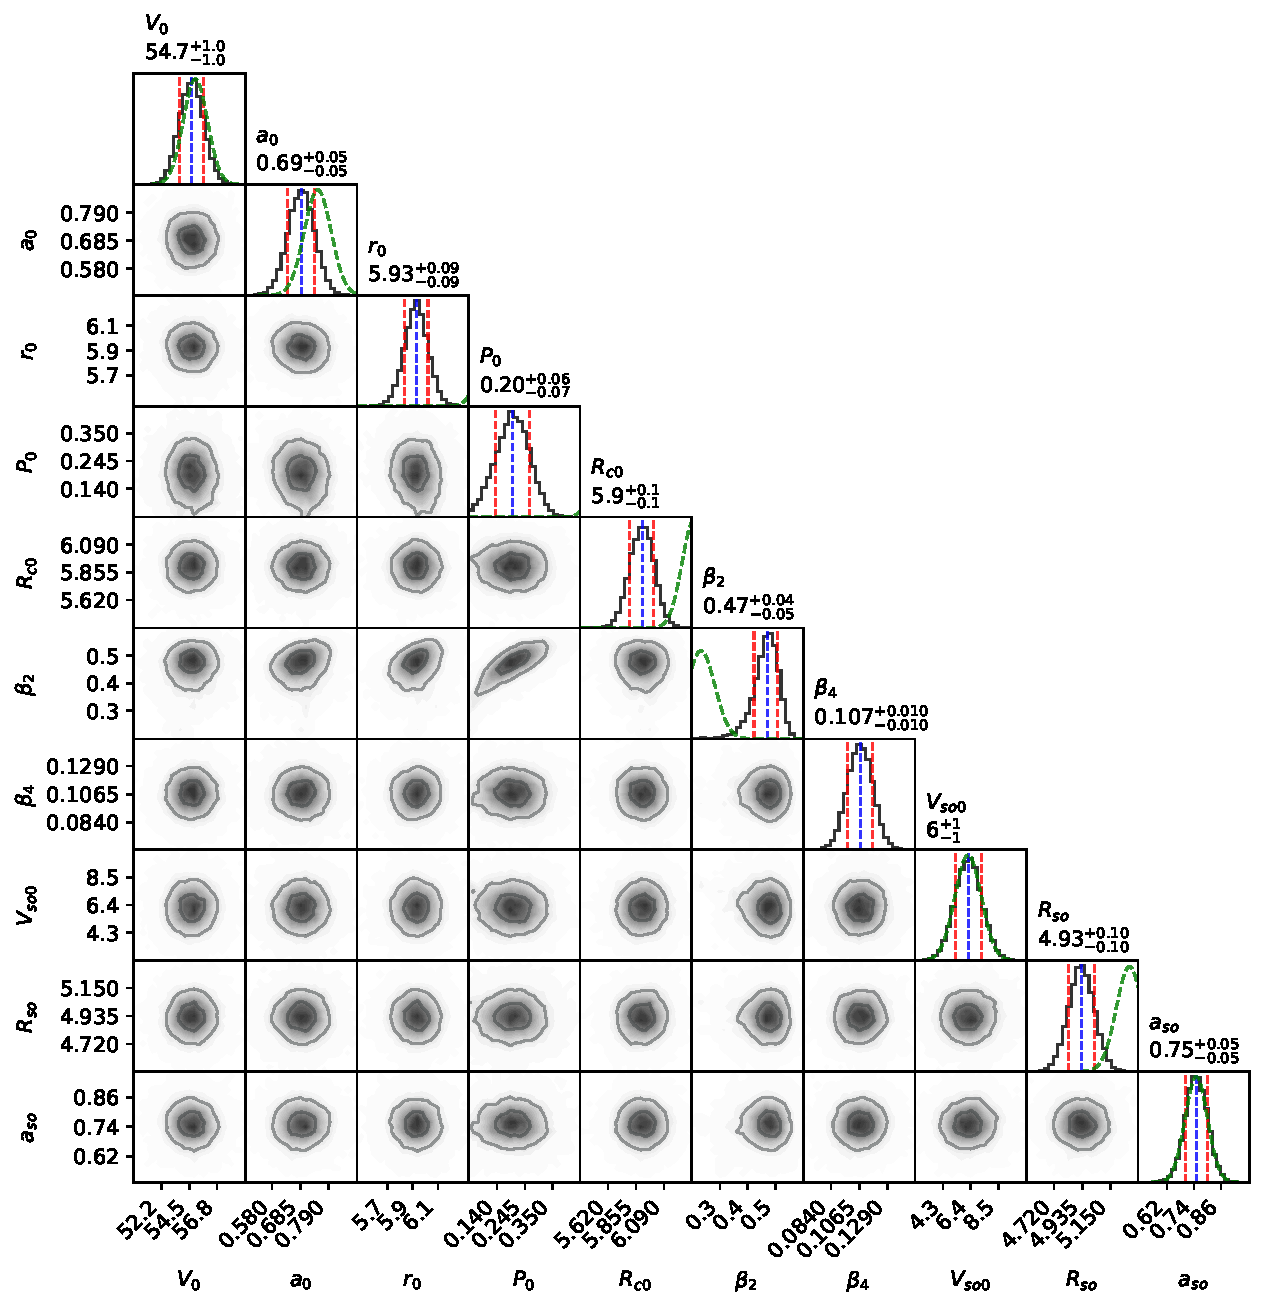
\includegraphics[width=0.8\textwidth]{Figures/figure15.pdf}
    \caption{117La的后验图(10000samples/sampler的正式运行)}
    \label{fig:15}
\end{figure}

然后是117La的参数敏感性图：
\begin{figure}[htbp]
    \centering
    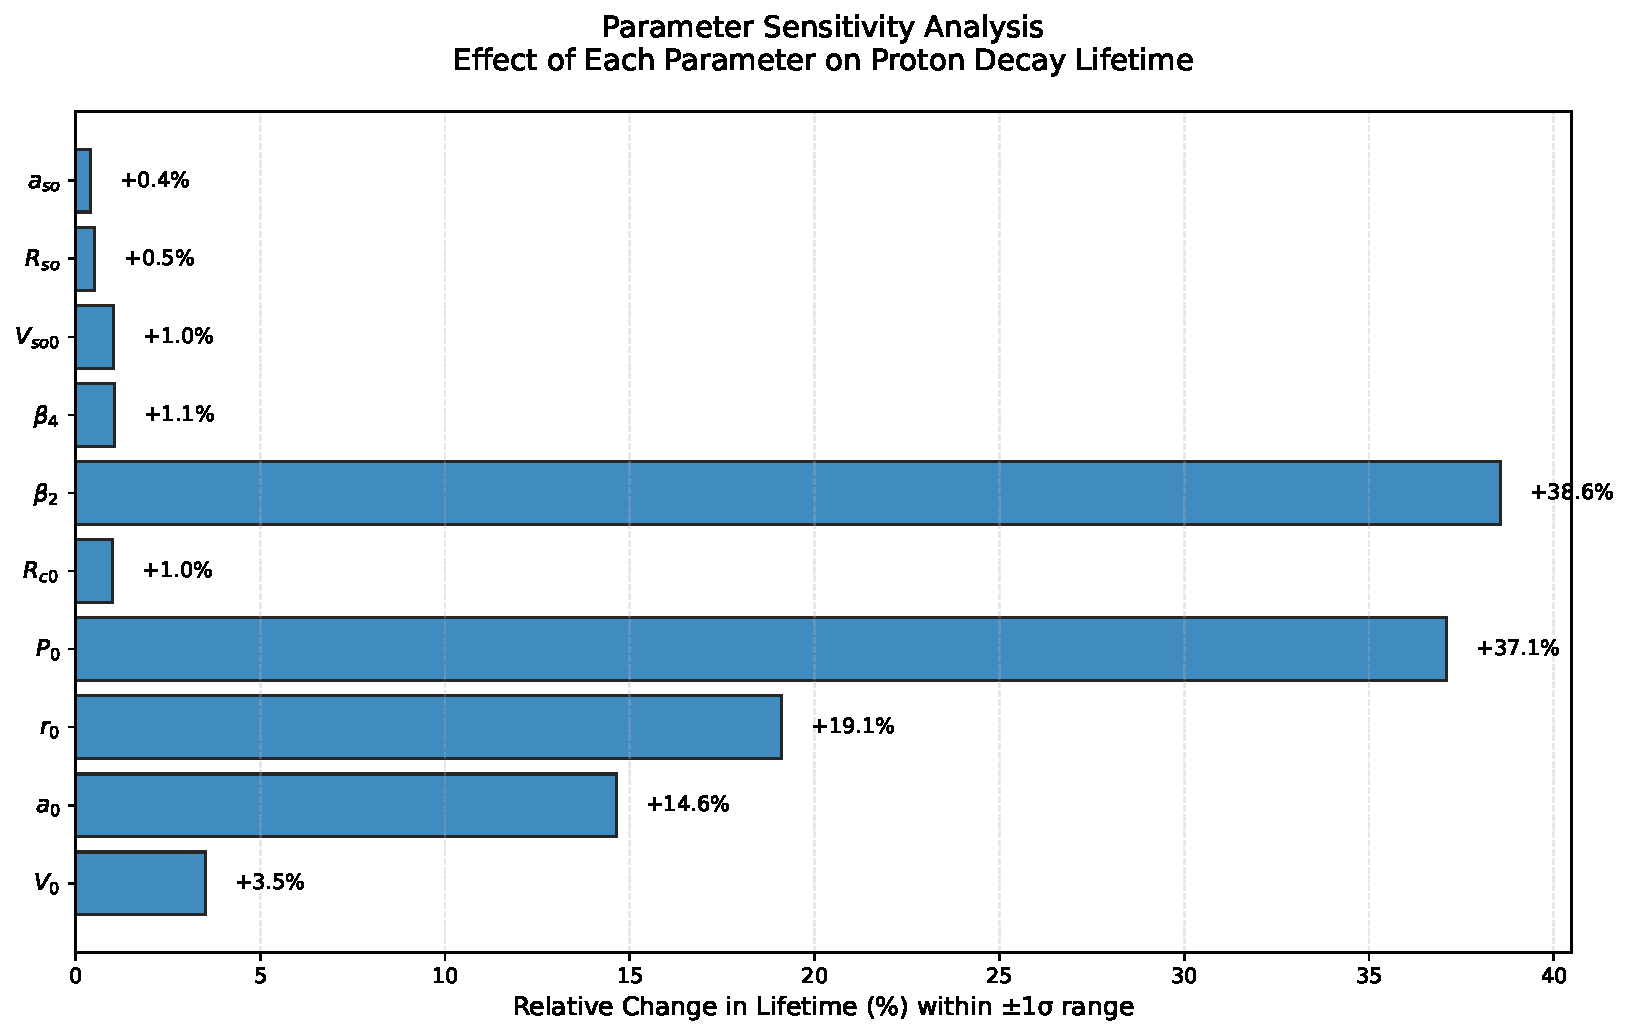
\includegraphics[width=0.8\textwidth]{Figures/figure16.pdf}
    \caption{117La的参数敏感性图(1sigma区间内的参数变化对半衰期的影响)}
    \label{fig:16}
\end{figure}

然后是117La的参数关联图：
\begin{figure}[htbp]
    \centering
    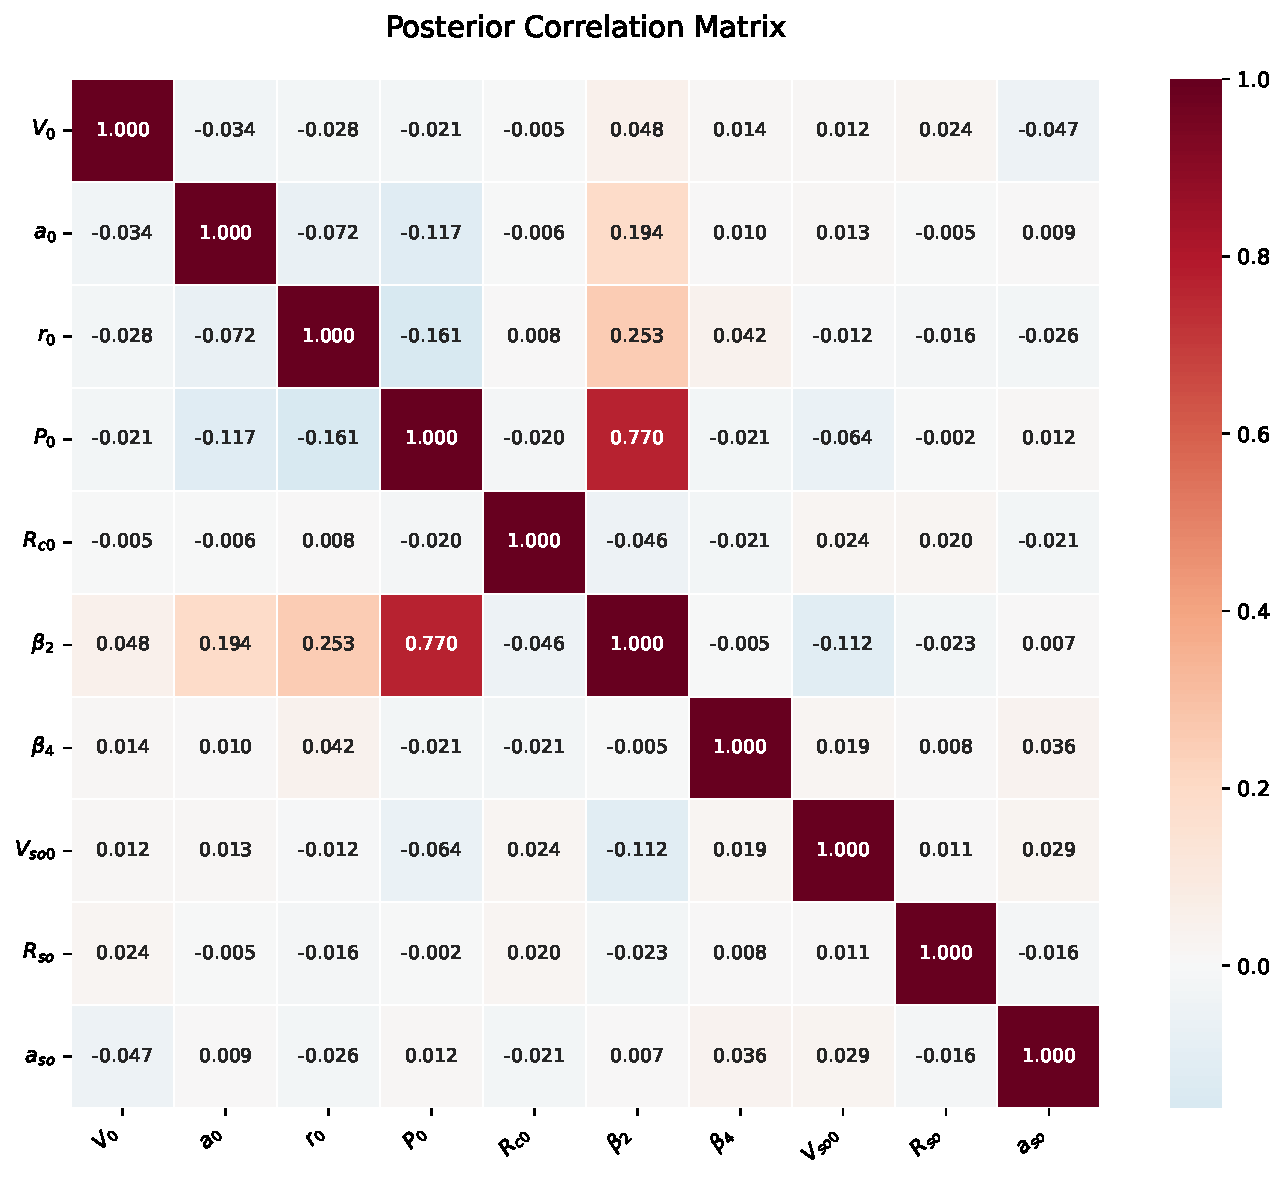
\includegraphics[width=0.8\textwidth]{Figures/figure17.pdf}
    \caption{117La的形变势能参数的关联矩阵,非对角项明显有一定值，体现了correlation}
    \label{fig:17}
\end{figure}
最后是117La的可观测量sigma区间：
\begin{verbatim}
========== Posterior Predictive Distribution of Lifetime ==========
experiment data: [0.0217] s
Number of posterior samples used: 5000
Mean lifetime      : 2.023e-02 s
Median lifetime    : 2.022e-02 s
Standard deviation : 1.882e-03 s
1σ error bar (±)   : 1.882e-03 s
2σ error bar (±)   : 3.763e-03 s
68% CI (1σ)        : [1.836e-02, 2.211e-02] s
95% CI (2σ)        : [1.661e-02, 2.392e-02] s
===================================================================
\end{verbatim}

然后对于121Pr进行研究，由于准备计算的时候查询nndc上，子核120Ce未有质量和Jpi信息，
所以去ame2020上查询了120Ce的理论预估质量，此外，在定质子的轨道角动量L的时候，我们查询121Pr
的Jpi信息，在nndc上有
\begin{figure}
    \centering
    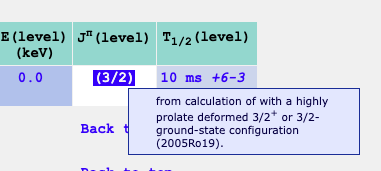
\includegraphics[width=0.8\textwidth]{Figures/figure21.png}
    \caption{121Pr的核数据查询结果,由于3/2-是基态，所以我们选择L=1的轨道进行计算}
    \label{fig:21}
\end{figure}

\clearpage

对于121Pr选取的计算参数如下：
\begin{verbatim}
#System of Proton Decay
#121Pr
e2=1.43997 ; hbarc=197.3269718 ; amu=931.49432
zp=59 ; Ap=121 ; mass_excess_p=-41.551 ; mp=Ap*amu+mass_excess_p        #Parent
z1=zp-1 ; A1=Ap-1 ; mass_excess_1=-49.730 ; m1=A1*amu+mass_excess_1    #1-> daughter
z2=1  ; A2=1   ; mass_excess_2=7.288971064 ; m2=A2*amu+mass_excess_2
Q=mp-m1-m2
print("Q=",Q)
mu=m1*m2/(m1+m2)
P0=0.122
#Potential

#Deformation
beta2 = 0.304  # quadrupole
beta4 = 0.087  # hexadecapole 

#Polarizaton
beta2tilde = 0  
beta4tilde = 0

#spin-orbit
Vso0=6.2 ; rso=1.01*(A1)**(1/3) ; aso=0.75 ; lambda_pi=np.sqrt(2)
L=2; S=0.5; J=1.5
print("rso=",rso)
#Vn
a0=0.75 ; r0=1.27*A1**(1/3)-0.1 ; V0=55
print("r0=",r0)
#Vc
Rc0 = 1.21 * A1**(1/3)          
print("Rc0=",Rc0)
#mesh
r = np.linspace(0.03, 30.0, 1000) # avoid too small r

# experiment data
y=np.array([10e-3])    # s
sigma=np.array([6e-3])

# Hyperparameters in Prior
    v0_mean=55; a0_mean=0.75; r0_mean=1.27*A1**(1/3)-0.1; p0_mean=0.311
    rc0_mean=1.21 * A1**(1/3); beta2_mean=0.304 ; beta4_mean=0.087
    vso0_mean=6.2; rso_mean=1.01*(A1)**(1/3); aso_mean=0.75

with multiprocessing.Pool() as pool:
    sampler = emcee.EnsembleSampler(nwalkers, M, log_posterior, 
    args=[y,sigma],a=2.0,pool=pool)
    state = sampler.run_mcmc(initial_positions, 200)
    sampler.reset()
    sampler.run_mcmc(state,10000)

\end{verbatim}


得到了121Pr的posterior图：
\begin{figure}[htbp]
    \centering
    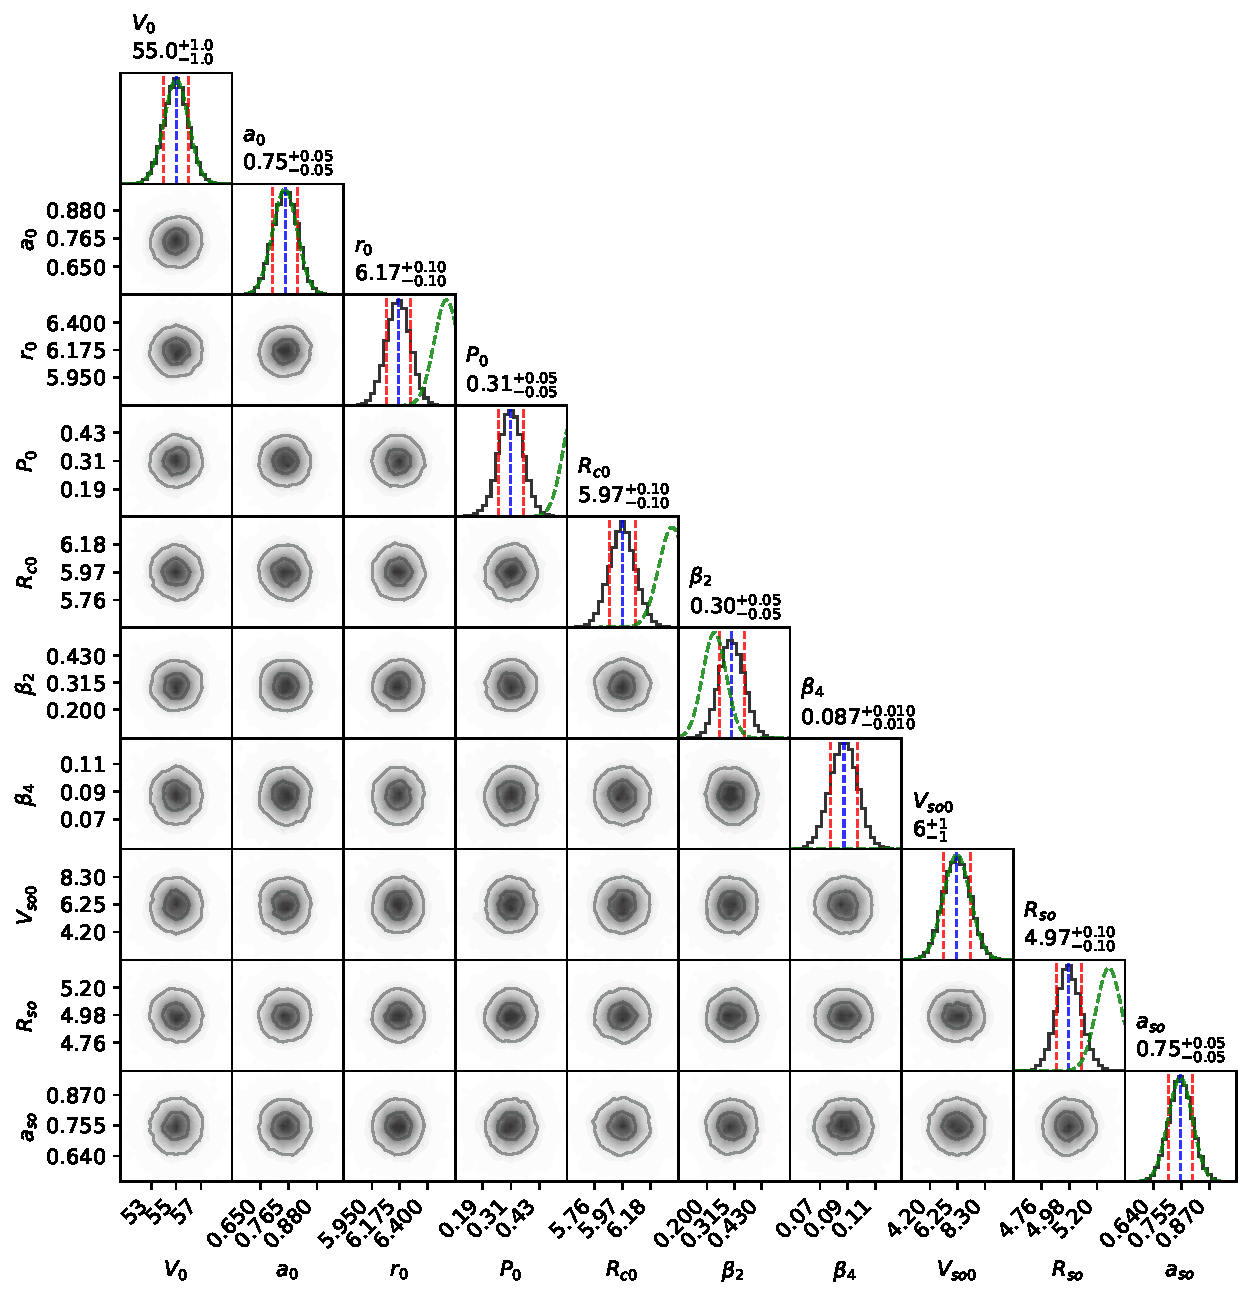
\includegraphics[width=0.8\textwidth]{Figures/figure18.pdf}
    \caption{121Pr的后验图(10000samples/sampler的正式运行)}
    \label{fig:18}
\end{figure}

然后是121Pr的参数敏感性图：
\begin{figure}[htbp]
    \centering
    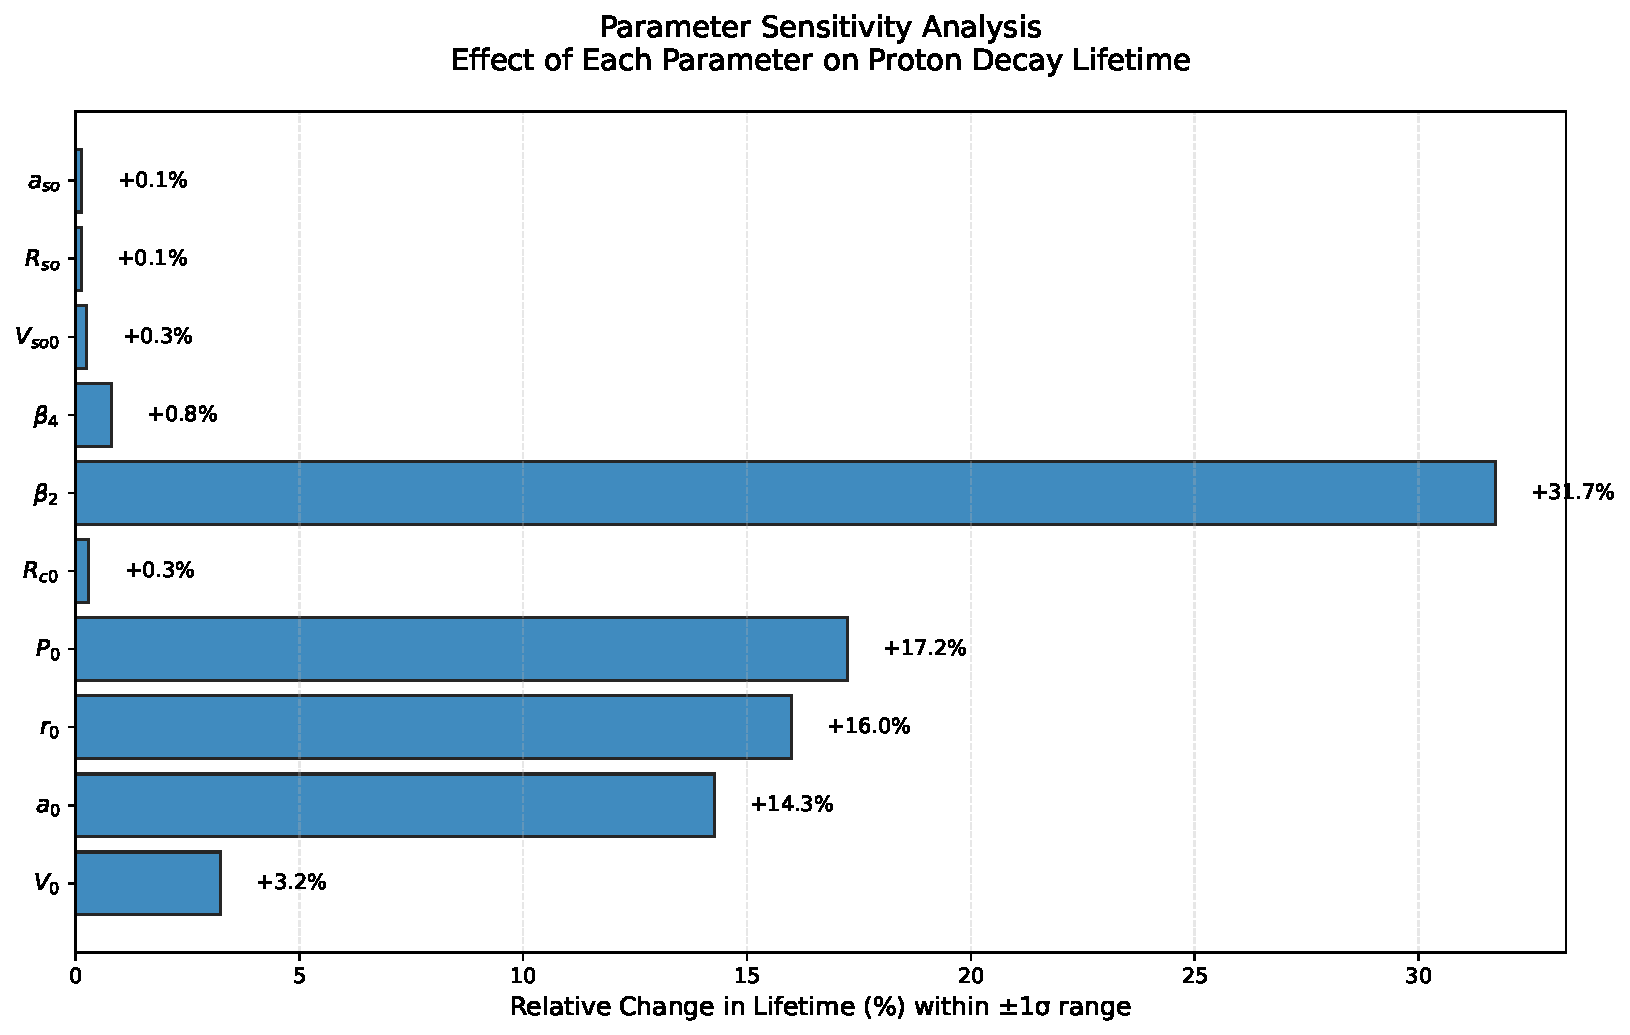
\includegraphics[width=0.8\textwidth]{Figures/figure19.pdf}
    \caption{121Pr的参数敏感性图(1sigma区间内的参数变化对半衰期的影响)}
    \label{fig:19}
\end{figure}

然后是121Pr的参数关联图：
\begin{figure}[htbp]
    \centering
    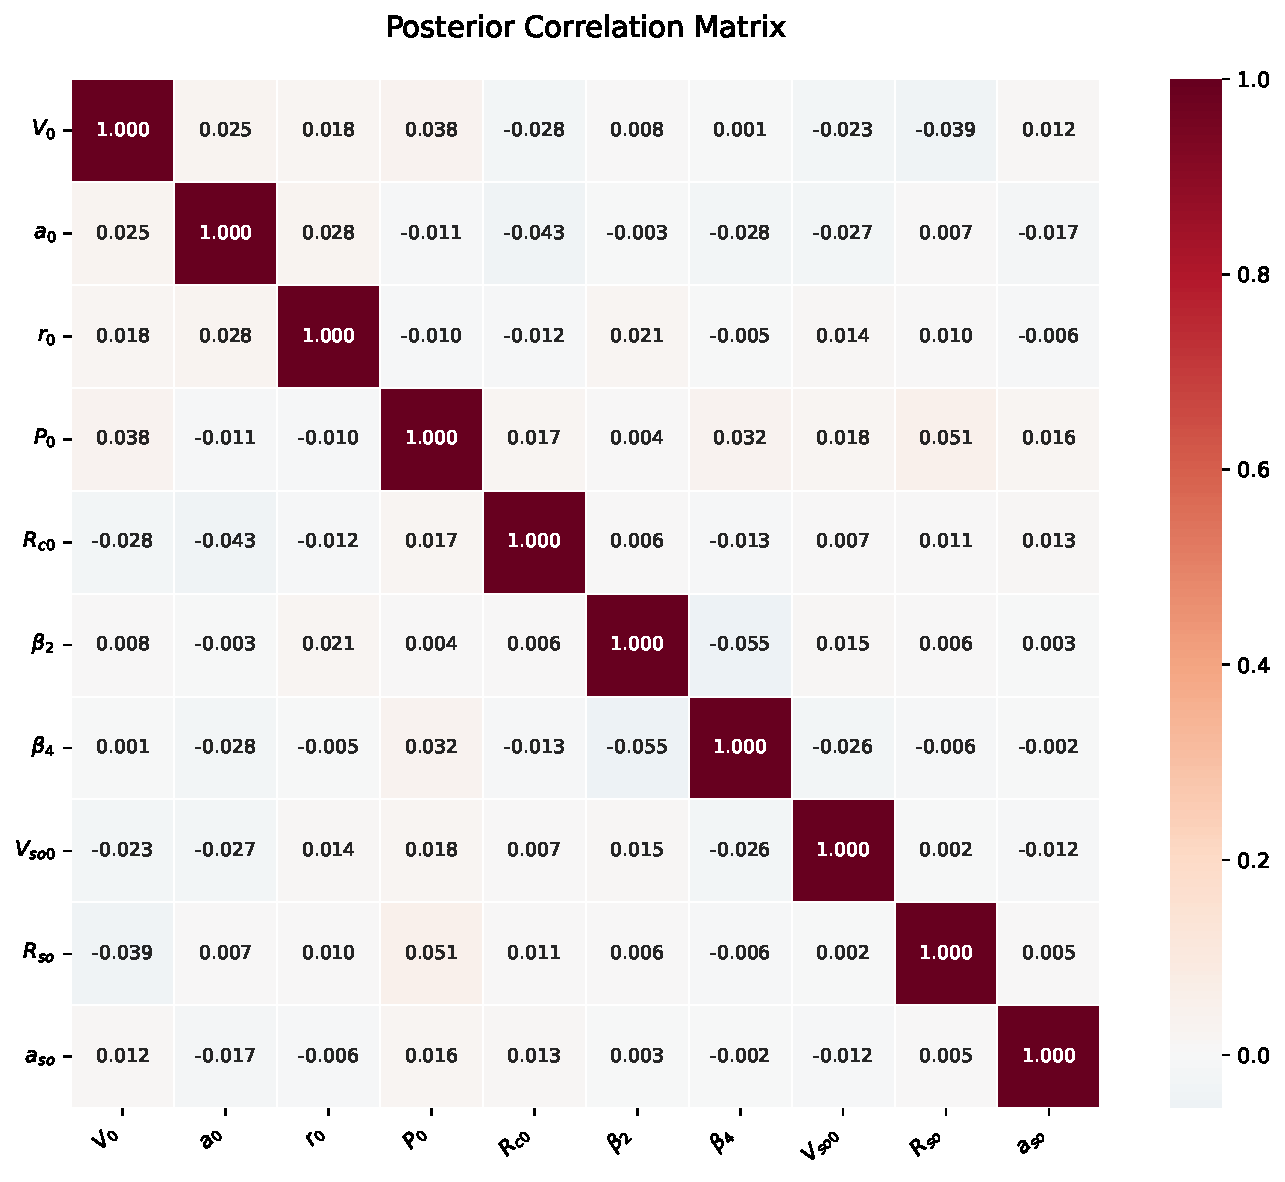
\includegraphics[width=0.8\textwidth]{Figures/figure20.pdf}
    \caption{121Pr的形变势能参数的关联矩阵} 
    \label{fig:20}
\end{figure}

\clearpage
然后对于131Eu进行计算

选取了131Eu的计算参数如下：
\begin{verbatim}
#System of Proton Decay
#131Eu
e2=1.43997 ; hbarc=197.3269718 ; amu=931.49432
zp=63 ; Ap=131 ; mass_excess_p=-39.5 ; mp=Ap*amu+mass_excess_p        #Parent
z1=zp-1 ; A1=Ap-1 ; mass_excess_1=-47.7 ; m1=A1*amu+mass_excess_1    #1-> daughter
z2=1  ; A2=1   ; mass_excess_2=7.288971064 ; m2=A2*amu+mass_excess_2
Q=mp-m1-m2
print("Q=",Q)
mu=m1*m2/(m1+m2)
P0=0.029
#Potential

#Deformation
beta2 = 0.331  # quadrupole
beta4 = 0.018  # hexadecapole 

#Polarizaton
beta2tilde = 0  
beta4tilde = 0

#spin-orbit
Vso0=6.2 ; rso=1.01*(A1)**(1/3) ; aso=0.75 ; lambda_pi=np.sqrt(2)
L=2; S=0.5; J=1.5
print("rso=",rso)
#Vn
a0=0.75 ; r0=1.27*A1**(1/3)-0.1 ; V0=55
print("r0=",r0)
#Vc
Rc0 = 1.21 * A1**(1/3)          
print("Rc0=",Rc0)
#mesh
r = np.linspace(0.03, 30.0, 1000) # avoid too small r

# experiment data
y=np.array([17.8e-3])    # s
sigma=np.array([1.9e-3])

# Hyperparameters in Prior
    v0_mean=55; a0_mean=0.75; r0_mean=1.27*A1**(1/3)-0.1; p0_mean=0.029
    rc0_mean=1.21 * A1**(1/3); beta2_mean=0.331 ; beta4_mean=0.018
    vso0_mean=6.2; rso_mean=1.01*(A1)**(1/3); aso_mean=0.75

with multiprocessing.Pool() as pool:
    sampler = emcee.EnsembleSampler(nwalkers, M, log_posterior,
     args=[y,sigma],a=2.0,pool=pool)
    state = sampler.run_mcmc(initial_positions, 200)
    sampler.reset()
    sampler.run_mcmc(state,10000)
\end{verbatim}
\clearpage
获得了131Eu的posterior图：
\begin{figure}[htbp]
    \centering
    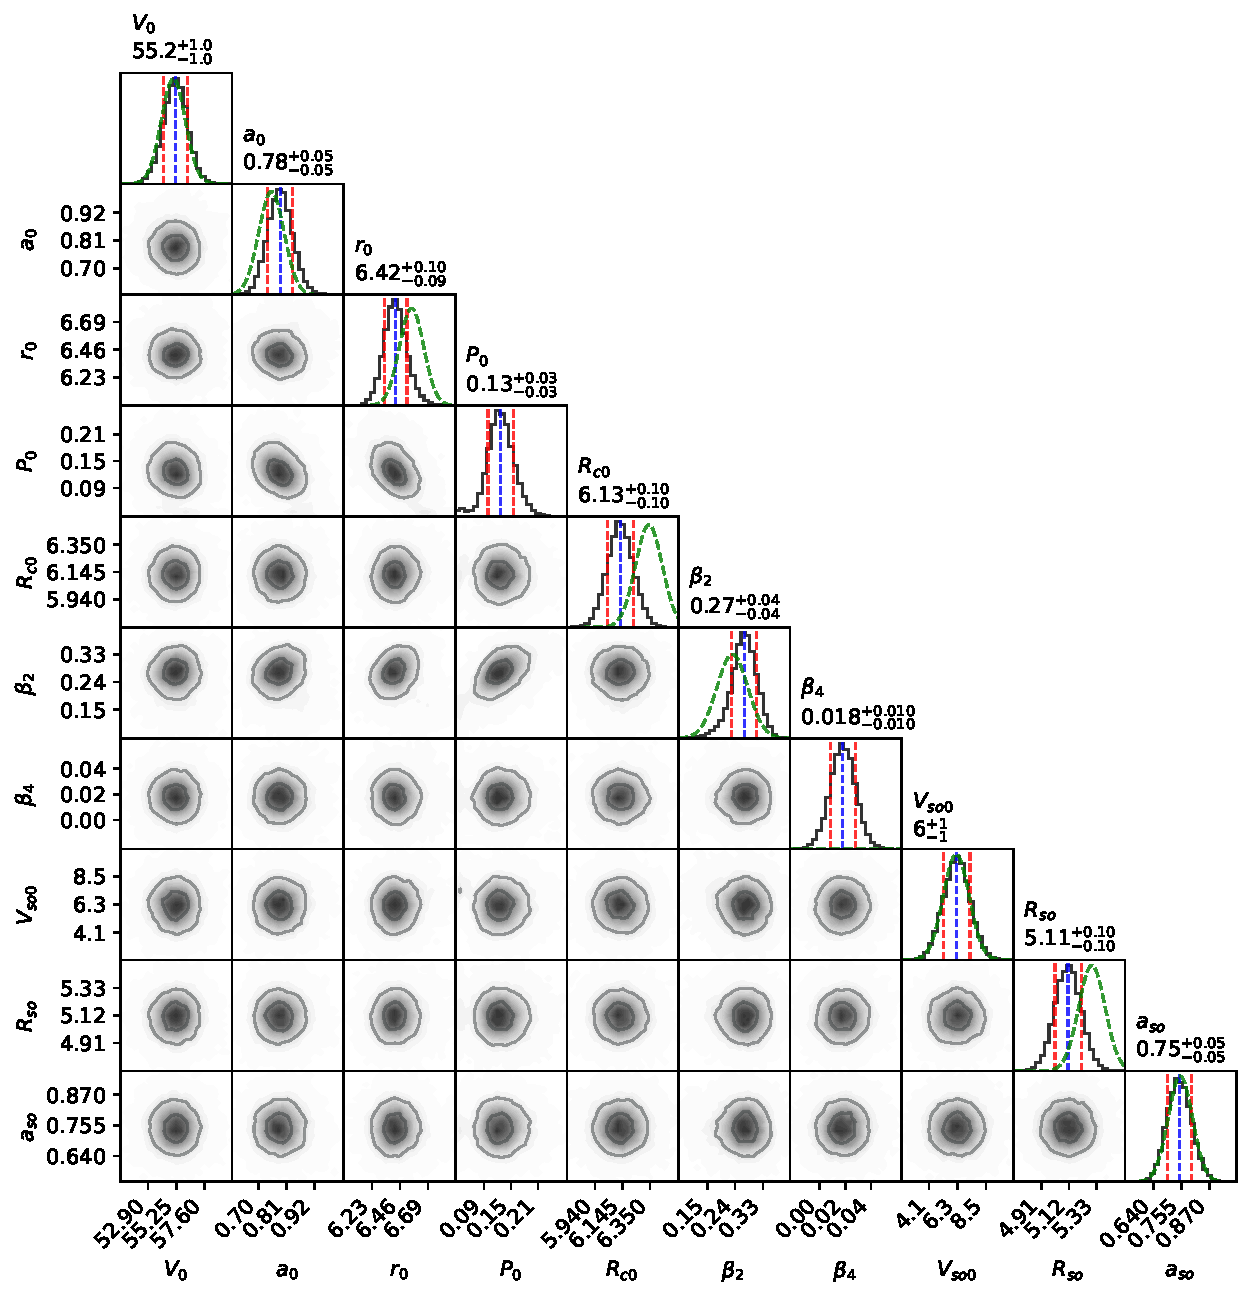
\includegraphics[width=0.8\textwidth]{Figures/figure22.pdf}
    \caption{131Eu的后验图(10000samples/sampler的正式运行   )}
    \label{fig:22}
\end{figure}

然后是131Eu的参数敏感性图：
\begin{figure}[htbp]
    \centering
    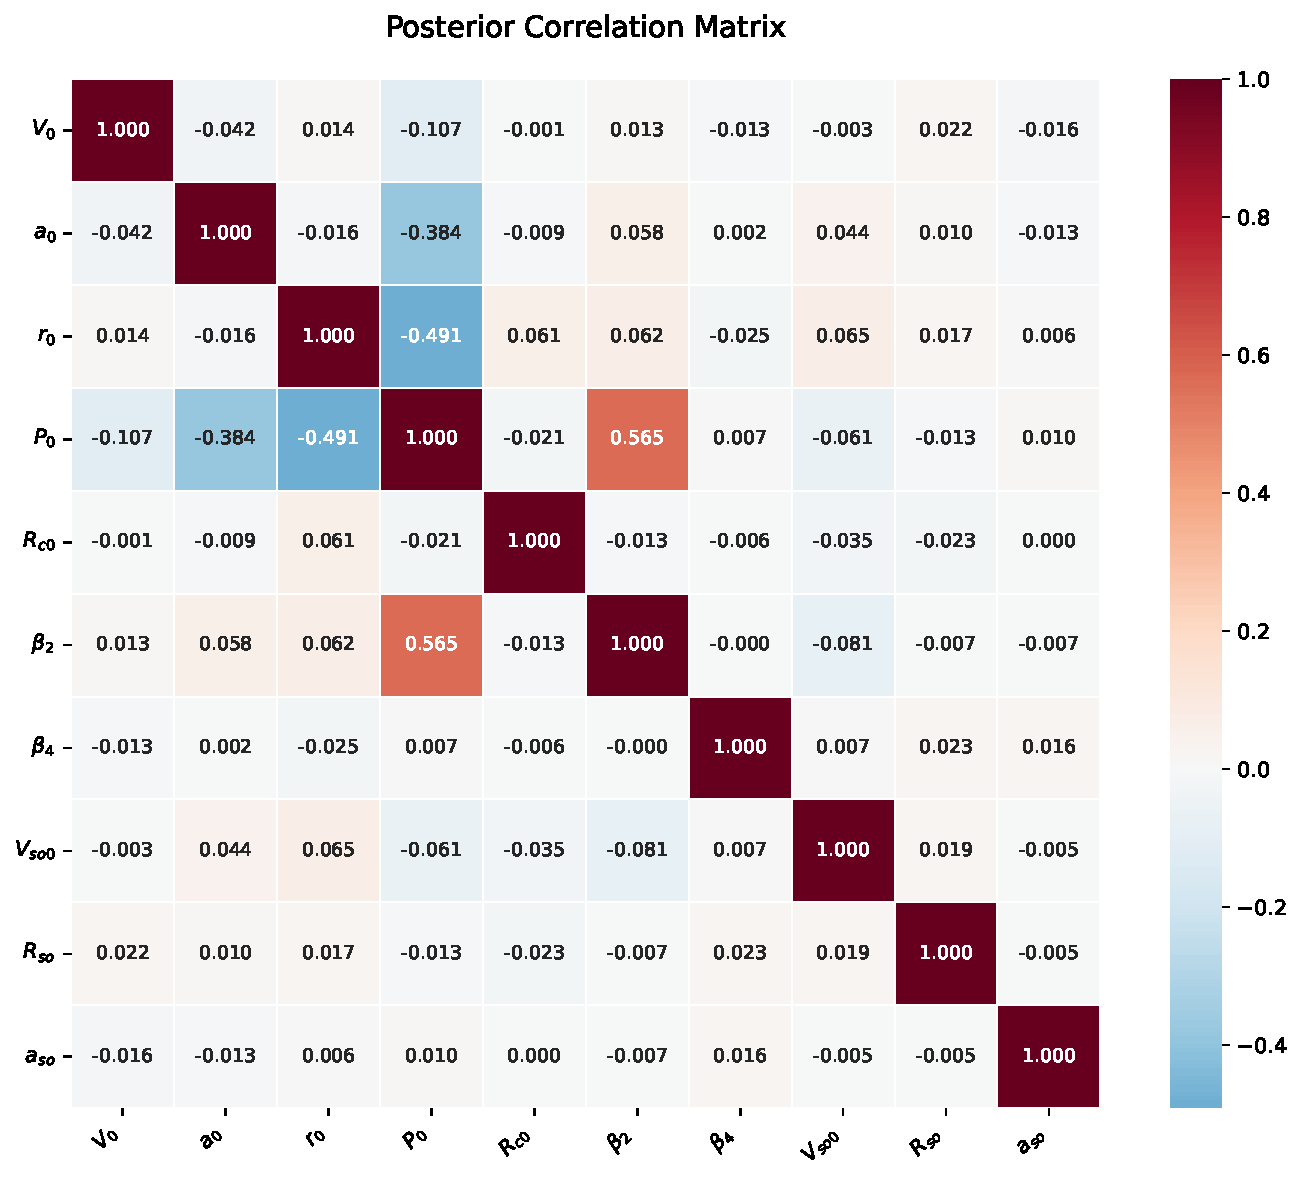
\includegraphics[width=0.8\textwidth]{Figures/figure23.pdf}
    \caption{131Eu的参数敏感性图(1sigma区间内的参数变化对半衰期的影响)}
    \label{fig:23}
\end{figure}

然后是131Eu的参数关联图：
\begin{figure}[htbp]
    \centering
    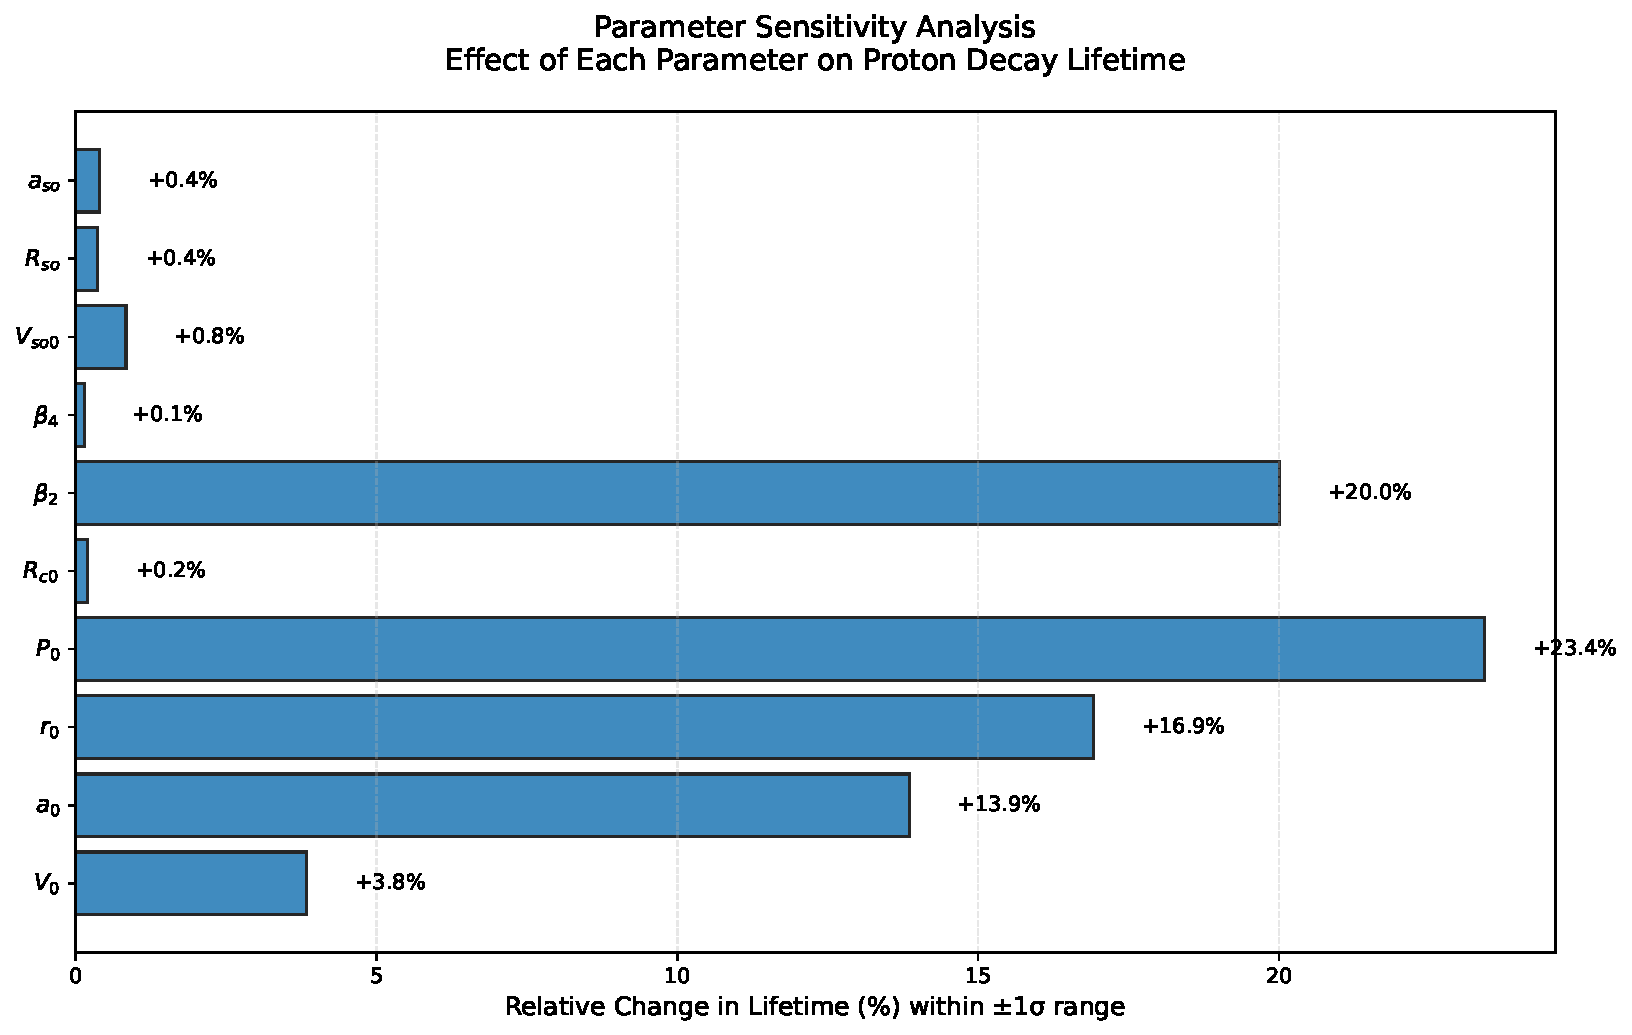
\includegraphics[width=0.8\textwidth]{Figures/figure24.pdf}
    \caption{131Eu的形变势能参数的关联矩阵}
    \label{fig:24}
\end{figure}

\clearpage
最后是131Eu的可观测量sigma区间：
\begin{verbatim}
========== Posterior Predictive Distribution of Lifetime ==========
experiment data: [0.0178] s
Number of posterior samples used: 5000
Mean lifetime      : 1.860e-02 s
Median lifetime    : 1.863e-02 s
Standard deviation : 1.843e-03 s
1σ error bar (±)   : 1.843e-03 s
2σ error bar (±)   : 3.686e-03 s
68% CI (1σ)        : [1.681e-02, 2.040e-02] s
95% CI (2σ)        : [1.489e-02, 2.217e-02] s
===================================================================
\end{verbatim}




然后是135Tb的计算，选取的计算参数如下：
\begin{verbatim}
#System of Proton Decay
#135Tb
e2=1.43997 ; hbarc=197.3269718 ; amu=931.49432
zp=65 ; Ap=135 ; mass_excess_p=-33.1 ; mp=Ap*amu+mass_excess_p        #Parent
z1=zp-1 ; A1=Ap-1 ; mass_excess_1=-41.5 ; m1=A1*amu+mass_excess_1    #1-> daughter
z2=1  ; A2=1   ; mass_excess_2=7.288971064 ; m2=A2*amu+mass_excess_2
Q=mp-m1-m2
print("Q=",Q)
mu=m1*m2/(m1+m2)
P0=0.028
#Potential

#Deformation
beta2 = 0.322  # quadrupole
beta4 = -0.037 # hexadecapole 

#Polarizaton
beta2tilde = 0  
beta4tilde = 0

#spin-orbit
Vso0=6.2 ; rso=1.01*(A1)**(1/3) ; aso=0.75 ; lambda_pi=np.sqrt(2)
L=3; S=0.5; J=3.5
print("rso=",rso)
#Vn
a0=0.75 ; r0=1.27*A1**(1/3)-0.1 ; V0=55
print("r0=",r0)
#Vc
Rc0 = 1.21 * A1**(1/3)          
print("Rc0=",Rc0)
#mesh
r = np.linspace(0.03, 30.0, 1000) # avoid too small r

# experiment data
y=np.array([0.94e-3])    # s
sigma=np.array([0.33e-3])

# Hyperparameters in Prior
    v0_mean=55; a0_mean=0.75; r0_mean=1.27*A1**(1/3)-0.1; p0_mean=0.028
    rc0_mean=1.21 * A1**(1/3); beta2_mean=0.322 ; beta4_mean=-0.037
    vso0_mean=6.2; rso_mean=1.01*(A1)**(1/3); aso_mean=0.75
with multiprocessing.Pool() as pool:
    sampler = emcee.EnsembleSampler(nwalkers, M, log_posterior, 
    args=[y,sigma],a=2.0,pool=pool)
    state = sampler.run_mcmc(initial_positions, 200)
    sampler.reset()
    sampler.run_mcmc(state,10000)

\end{verbatim}


获得了135Tb的posterior图：
\begin{figure}[htbp]
    \centering
    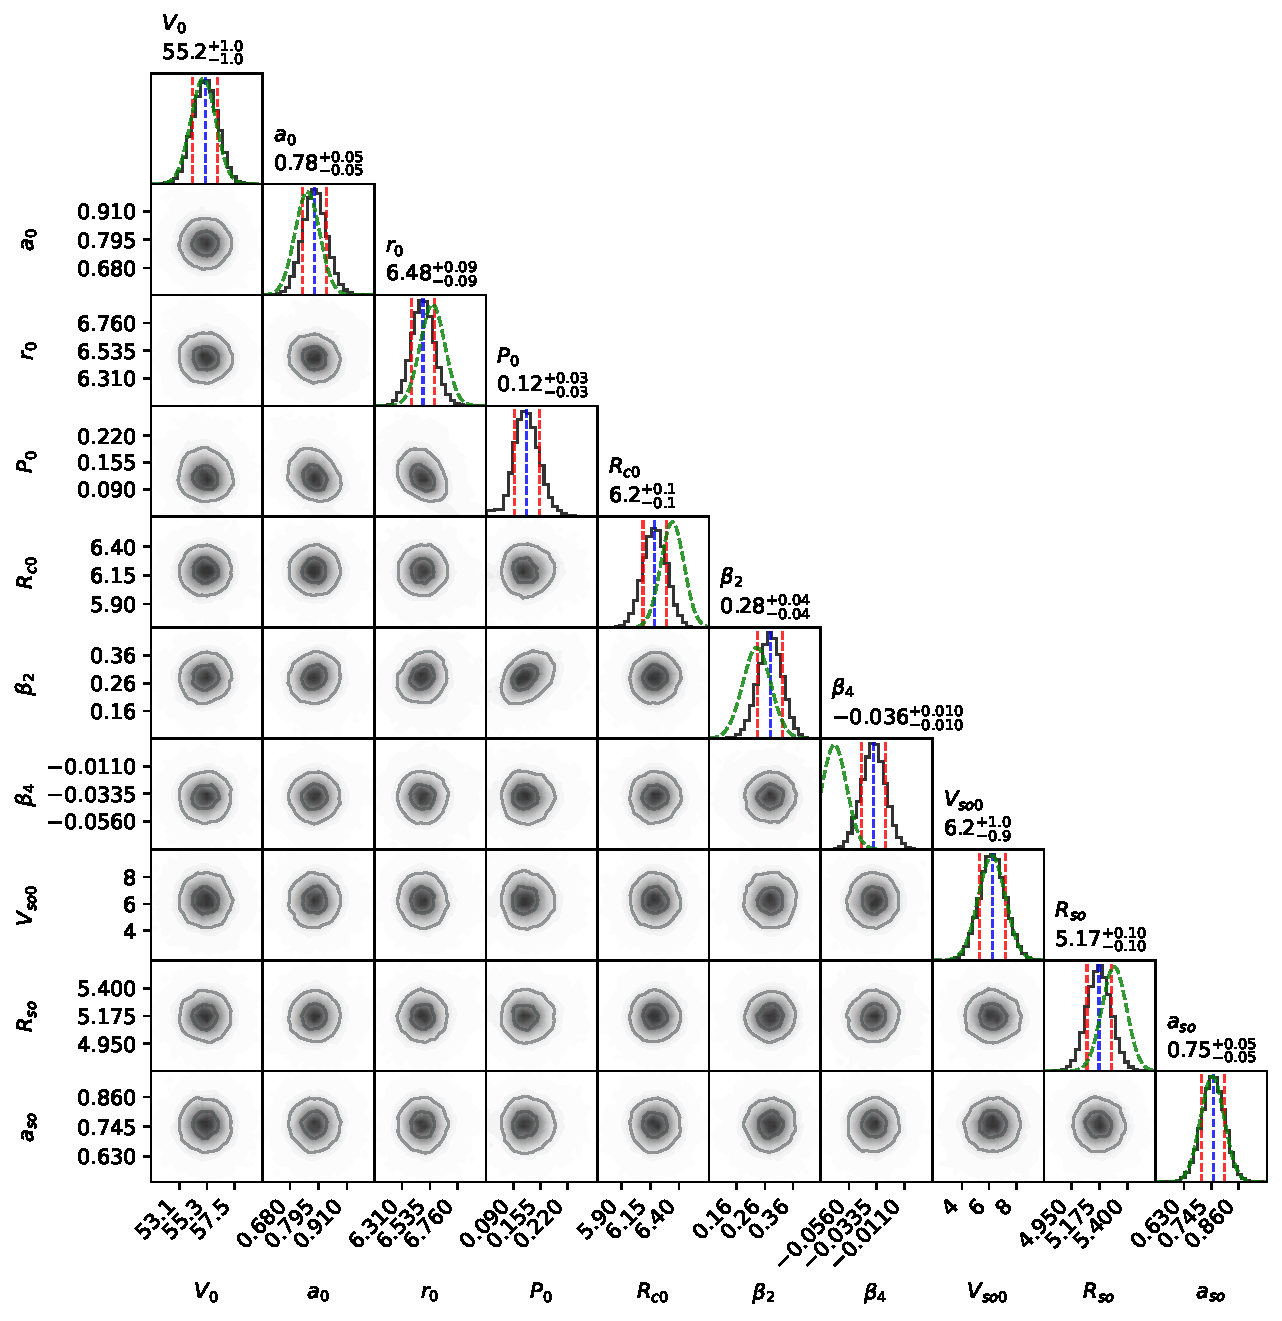
\includegraphics[width=0.8\textwidth]{Figures/figure25.pdf}
    \caption{135Tb的后验图(10000samples/sampler的正式运行)}
    \label{fig:25}
\end{figure}

然后是135Tb的参数敏感性图：
\begin{figure}[htbp]
    \centering
    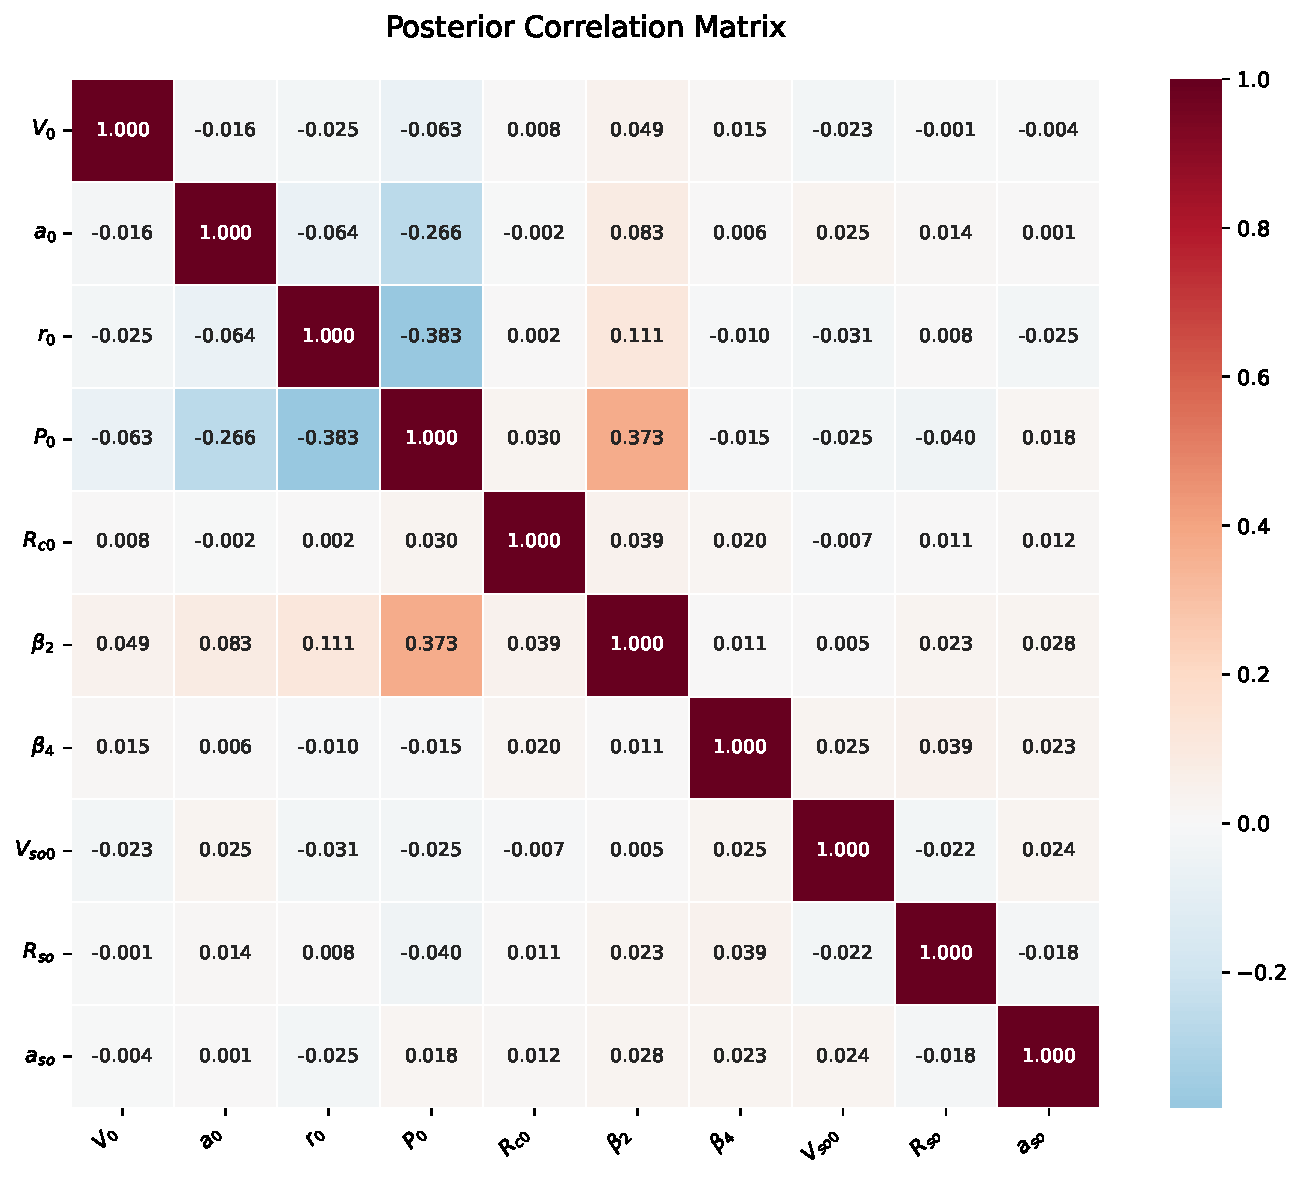
\includegraphics[width=0.8\textwidth]{Figures/figure26.pdf}
    \caption{135Tb的参数敏感性图(1sigma区间内的参数变化对半衰期的影响)}
    \label{fig:26}
\end{figure}

然后是135Tb的参数关联图：
\begin{figure}[htbp]
    \centering
    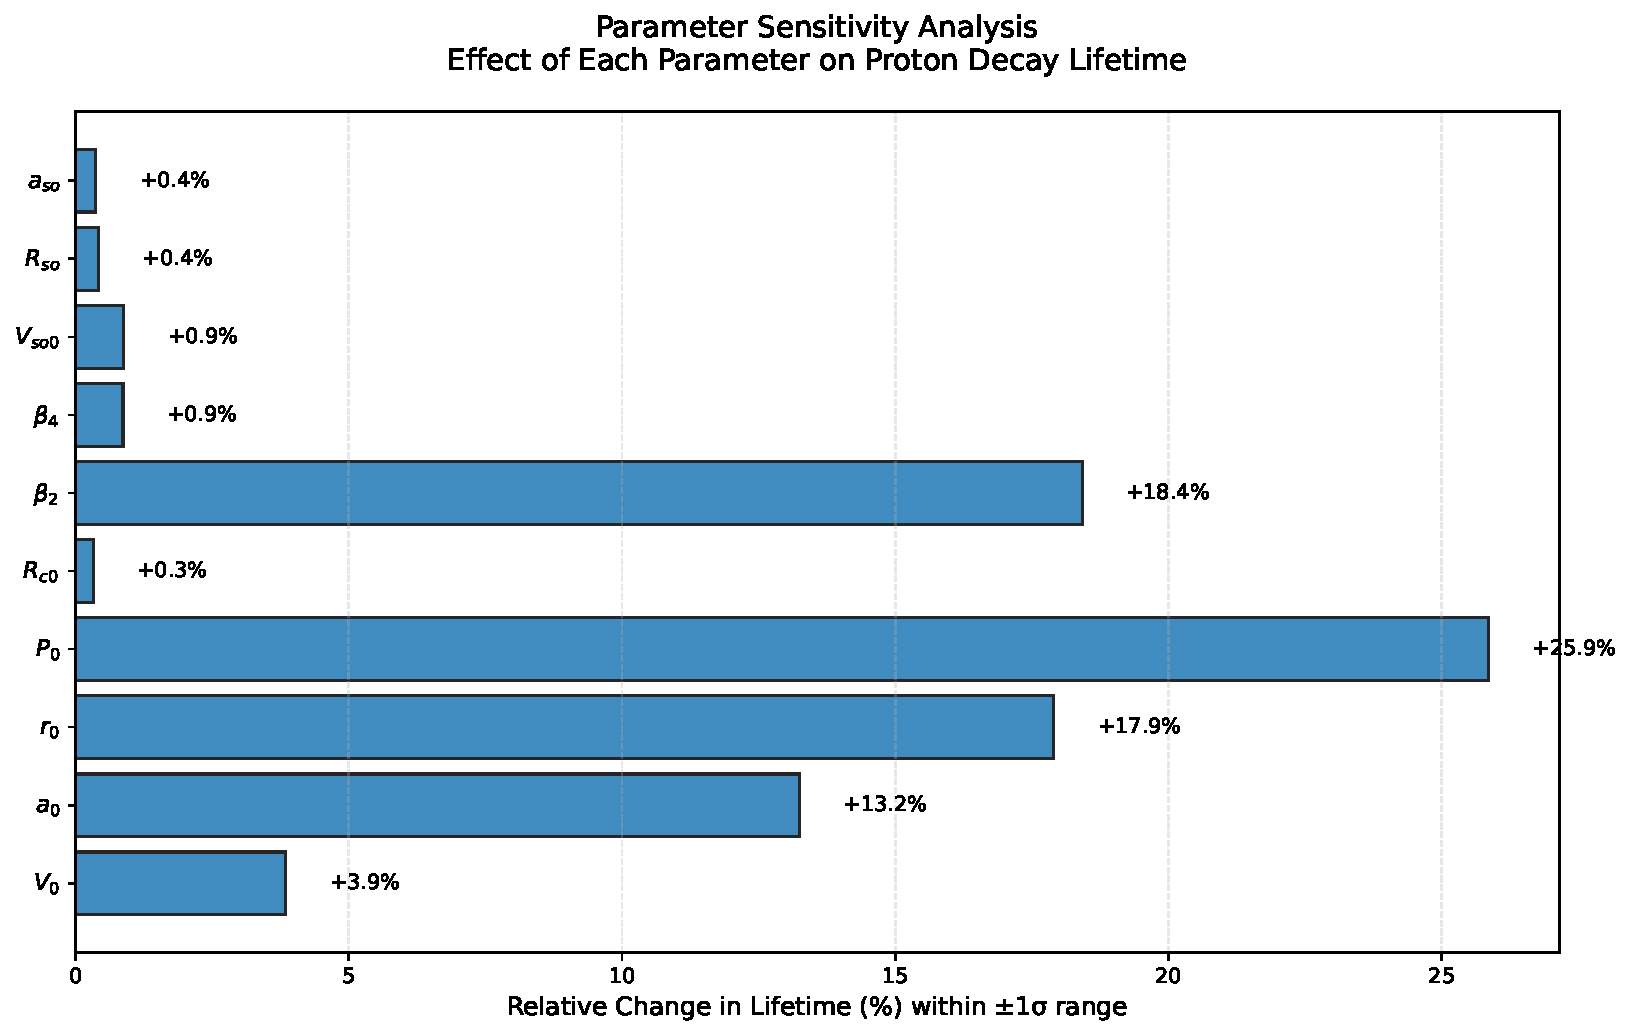
\includegraphics[width=0.8\textwidth]{Figures/figure27.pdf}
    \caption{135Tb的形变势能参数的关联矩阵}
    \label{fig:27}
\end{figure}
\clearpage
最后是135Tb的可观测量sigma区间：
\begin{verbatim}
========== Posterior Predictive Distribution of Lifetime ==========
experiment data: [0.00094] s
Number of posterior samples used: 5000
Mean lifetime      : 1.266e-03 s
Median lifetime    : 1.251e-03 s
Standard deviation : 2.777e-04 s
1σ error bar (±)   : 2.777e-04 s
2σ error bar (±)   : 5.553e-04 s
68% CI (1σ)        : [9.946e-04, 1.539e-03] s
95% CI (2σ)        : [7.691e-04, 1.848e-03] s
===================================================================
\end{verbatim}

然后对141Ho进行研究，选取的计算参数如下：
\begin{verbatim}
#System of Proton Decay
#141Ho
e2=1.43997 ; hbarc=197.3269718 ; amu=931.49432
zp=67 ; Ap=141 ; mass_excess_p=-34.4 ; mp=Ap*amu+mass_excess_p        #Parent
z1=zp-1 ; A1=Ap-1 ; mass_excess_1=-42.8 ; m1=A1*amu+mass_excess_1    #1-> daughter
z2=1  ; A2=1   ; mass_excess_2=7.288971064 ; m2=A2*amu+mass_excess_2
Q=mp-m1-m2
print("Q=",Q)
mu=m1*m2/(m1+m2)
P0=0.008
#Potential

#Deformation
beta2 = 0.253  # quadrupole
beta4 = -0.039 # hexadecapole 

#Polarizaton
beta2tilde = 0  
beta4tilde = 0

#spin-orbit
Vso0=6.2 ; rso=1.01*(A1)**(1/3) ; aso=0.75 ; lambda_pi=np.sqrt(2)
L=3; S=0.5; J=3.5
print("rso=",rso)
#Vn
a0=0.75 ; r0=1.27*A1**(1/3)-0.1 ; V0=55
print("r0=",r0)
#Vc
Rc0 = 1.21 * A1**(1/3)          
print("Rc0=",Rc0)
#mesh
r = np.linspace(0.03, 30.0, 1000) # avoid too small r

# experiment data
y=np.array([4.1e-3])    # s
sigma=np.array([0.1e-3])

# Hyperparameters in Prior
    v0_mean=55; a0_mean=0.75; r0_mean=1.27*A1**(1/3)-0.1; p0_mean=0.008
    rc0_mean=1.21 * A1**(1/3); beta2_mean=0.253 ; beta4_mean=-0.039
    vso0_mean=6.2; rso_mean=1.01*(A1)**(1/3); aso_mean=0.75
with multiprocessing.Pool() as pool:
    sampler = emcee.EnsembleSampler(nwalkers, M, log_posterior, 
    args=[y,sigma],a=2.0,pool=pool)
    state = sampler.run_mcmc(initial_positions, 200)
    sampler.reset()
    sampler.run_mcmc(state,10000)


\end{verbatim}

获得了141Ho的posterior图：
\begin{figure}[htbp]
    \centering
    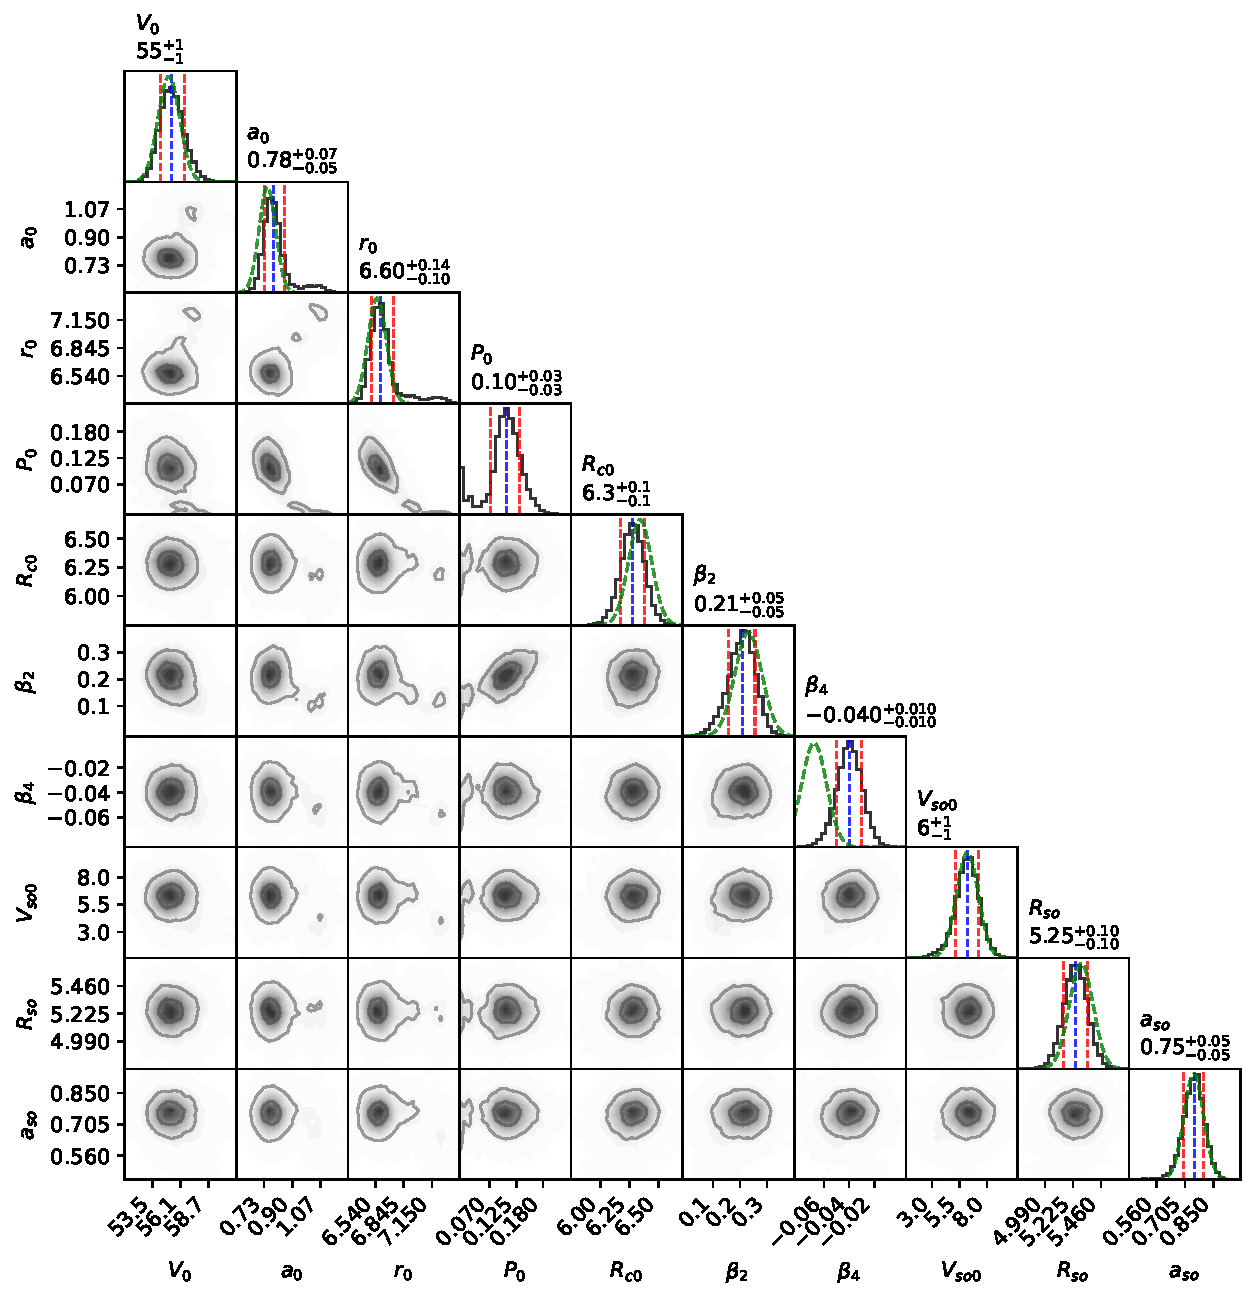
\includegraphics[width=0.8\textwidth]{Figures/figure28.pdf}
    \caption{141Ho的后验图(10000samples/sampler的正式运行)}
    \label{fig:28}
\end{figure}

然后是141Ho的参数关联图：
\begin{figure}[htbp]
    \centering
    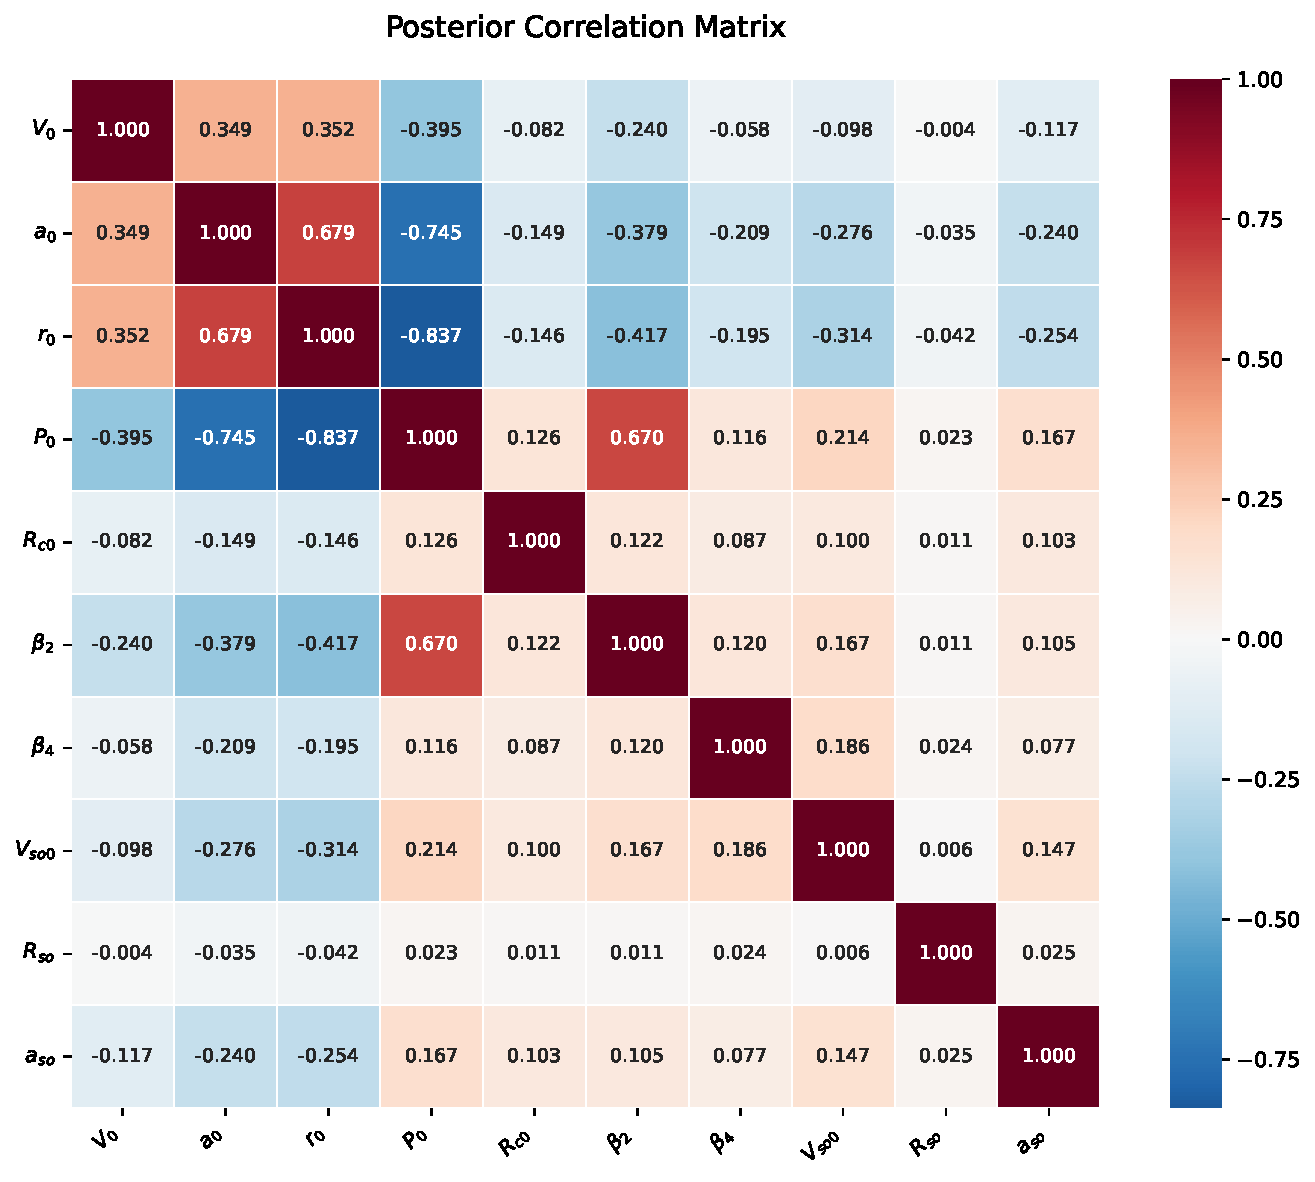
\includegraphics[width=0.8\textwidth]{Figures/figure29.pdf}
    \caption{141Ho的形变势能参数的关联矩阵}
    \label{fig:29}
\end{figure}

然后是141Ho的参数敏感性图：
\begin{figure}[htbp]
    \centering
    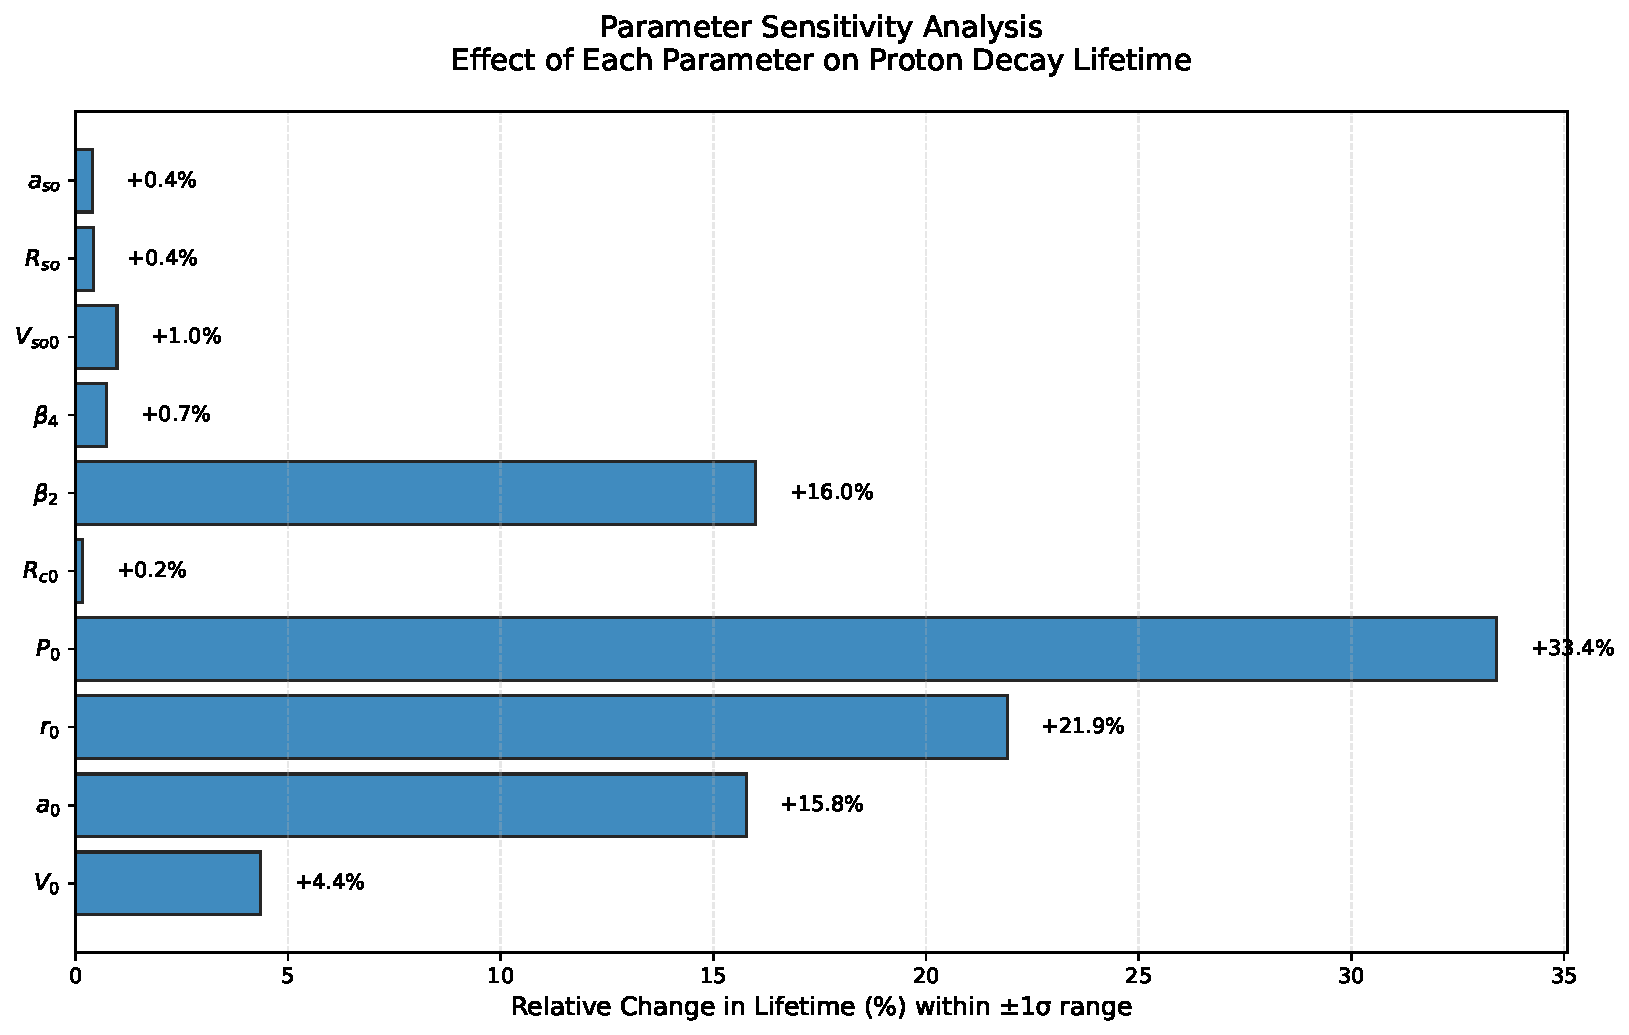
\includegraphics[width=0.8\textwidth]{Figures/figure30.pdf}
    \caption{141Ho的参数敏感性图(1sigma区间内的参数变化对半衰期的影响)}
    \label{fig:30}
\end{figure}




\clearpage
最后是141Ho的可观测量sigma区间：
\begin{verbatim}
========== Posterior Predictive Distribution of Lifetime ==========
experiment data: [0.0041] s
Number of posterior samples used: 5000
Mean lifetime      : 4.128e-03 s
Median lifetime    : 4.125e-03 s
Standard deviation : 1.083e-04 s
1σ error bar (±)   : 1.083e-04 s
2σ error bar (±)   : 2.167e-04 s
68% CI (1σ)        : [4.021e-03, 4.235e-03] s
95% CI (2σ)        : [3.916e-03, 4.346e-03] s
===================================================================
\end{verbatim}


然后对151Lu进行研究，选取的计算参数如下：
\begin{verbatim}
#System of Proton Decay
#151Lu
e2=1.43997 ; hbarc=197.3269718 ; amu=931.49432
zp=71 ; Ap=151 ; mass_excess_p=-30.3 ; mp=Ap*amu+mass_excess_p        #Parent
z1=zp-1 ; A1=Ap-1 ; mass_excess_1=-38.8 ; m1=A1*amu+mass_excess_1    #1-> daughter
z2=1  ; A2=1   ; mass_excess_2=7.288971064 ; m2=A2*amu+mass_excess_2
Q=mp-m1-m2
print("Q=",Q)
mu=m1*m2/(m1+m2)
P0=0.490
#Potential

#Deformation
beta2 = -0.167  # quadrupole
beta4 = -0.035 # hexadecapole 

#Polarizaton
beta2tilde = 0  
beta4tilde = 0

#spin-orbit
Vso0=6.2 ; rso=1.01*(A1)**(1/3) ; aso=0.75 ; lambda_pi=np.sqrt(2)
L=5; S=0.5; J=5.5
print("rso=",rso)
#Vn
a0=0.75 ; r0=1.27*A1**(1/3)-0.1 ; V0=55
print("r0=",r0)
#Vc
Rc0 = 1.21 * A1**(1/3)          
print("Rc0=",Rc0)
#mesh
r = np.linspace(0.03, 30.0, 1000) # avoid too small r

# experiment data
y=np.array([79e-3])    # s
sigma=np.array([1e-3])

# Hyperparameters in Prior
    v0_mean=55; a0_mean=0.75; r0_mean=1.27*A1**(1/3)-0.1; p0_mean=0.490
    rc0_mean=1.21 * A1**(1/3); beta2_mean=-0.167 ; beta4_mean=-0.035
    vso0_mean=6.2; rso_mean=1.01*(A1)**(1/3); aso_mean=0.75
with multiprocessing.Pool() as pool:
    sampler = emcee.EnsembleSampler(nwalkers, M, log_posterior, 
    args=[y,sigma],a=2.0,pool=pool)
    state = sampler.run_mcmc(initial_positions, 200)
    sampler.reset()
    sampler.run_mcmc(state,10000)

\end{verbatim}


获得了151Lu的posterior图：

\begin{figure}
    \centering
    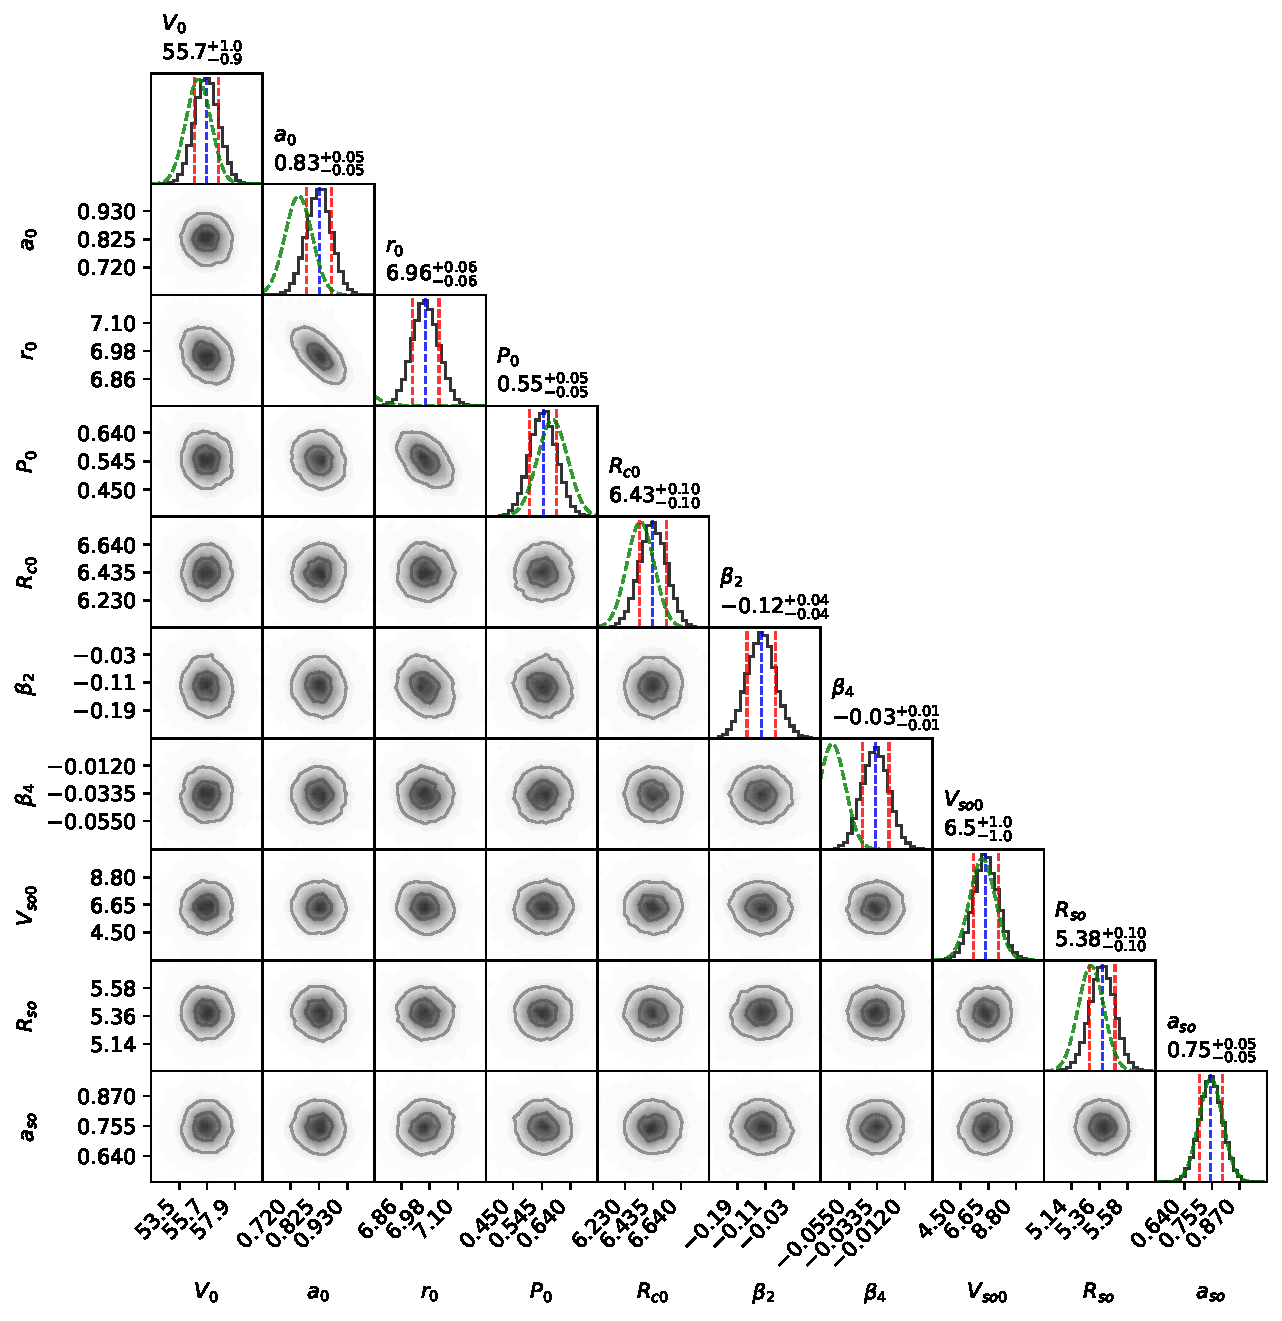
\includegraphics[width=0.8\textwidth]{Figures/figure31.pdf}
    \caption{151Lu的后验图(10000samples/sampler的正式运行)}
    \label{fig:31}
\end{figure}

然后是151Lu的参数关联图：   
\begin{figure}
    \centering
    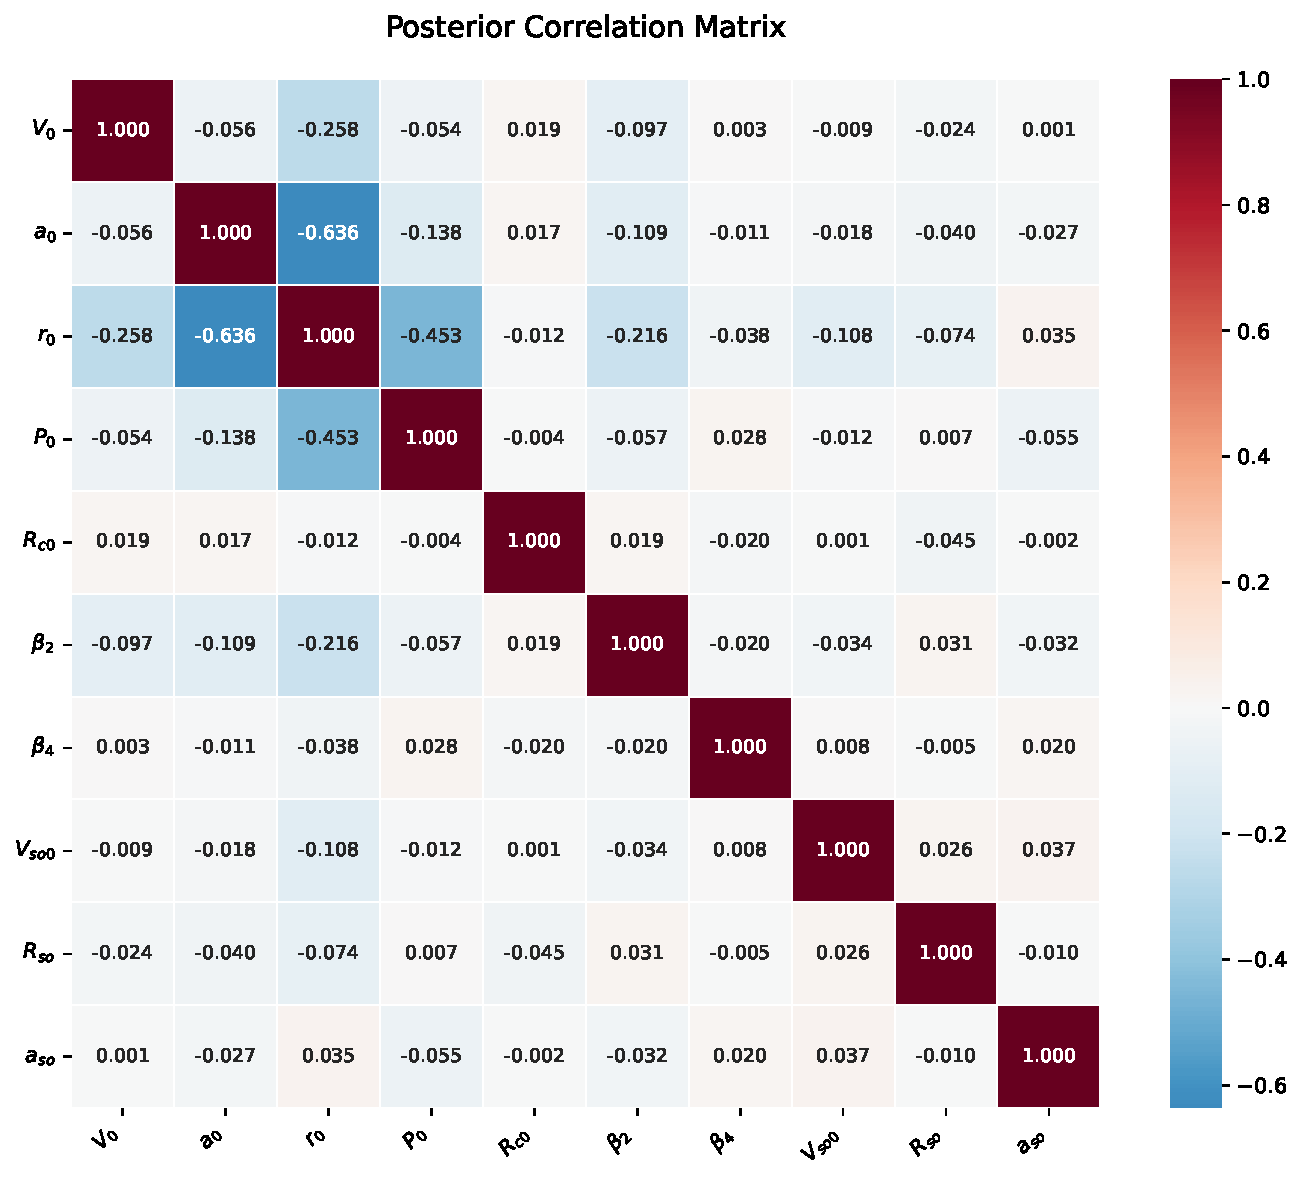
\includegraphics[width=0.8\textwidth]{Figures/figure32.pdf}
    \caption{151Lu的形变势能参数的关联矩阵}
    \label{fig:32}
\end{figure}

然后是151Lu的参数敏感性图：
\begin{figure}
    \centering
    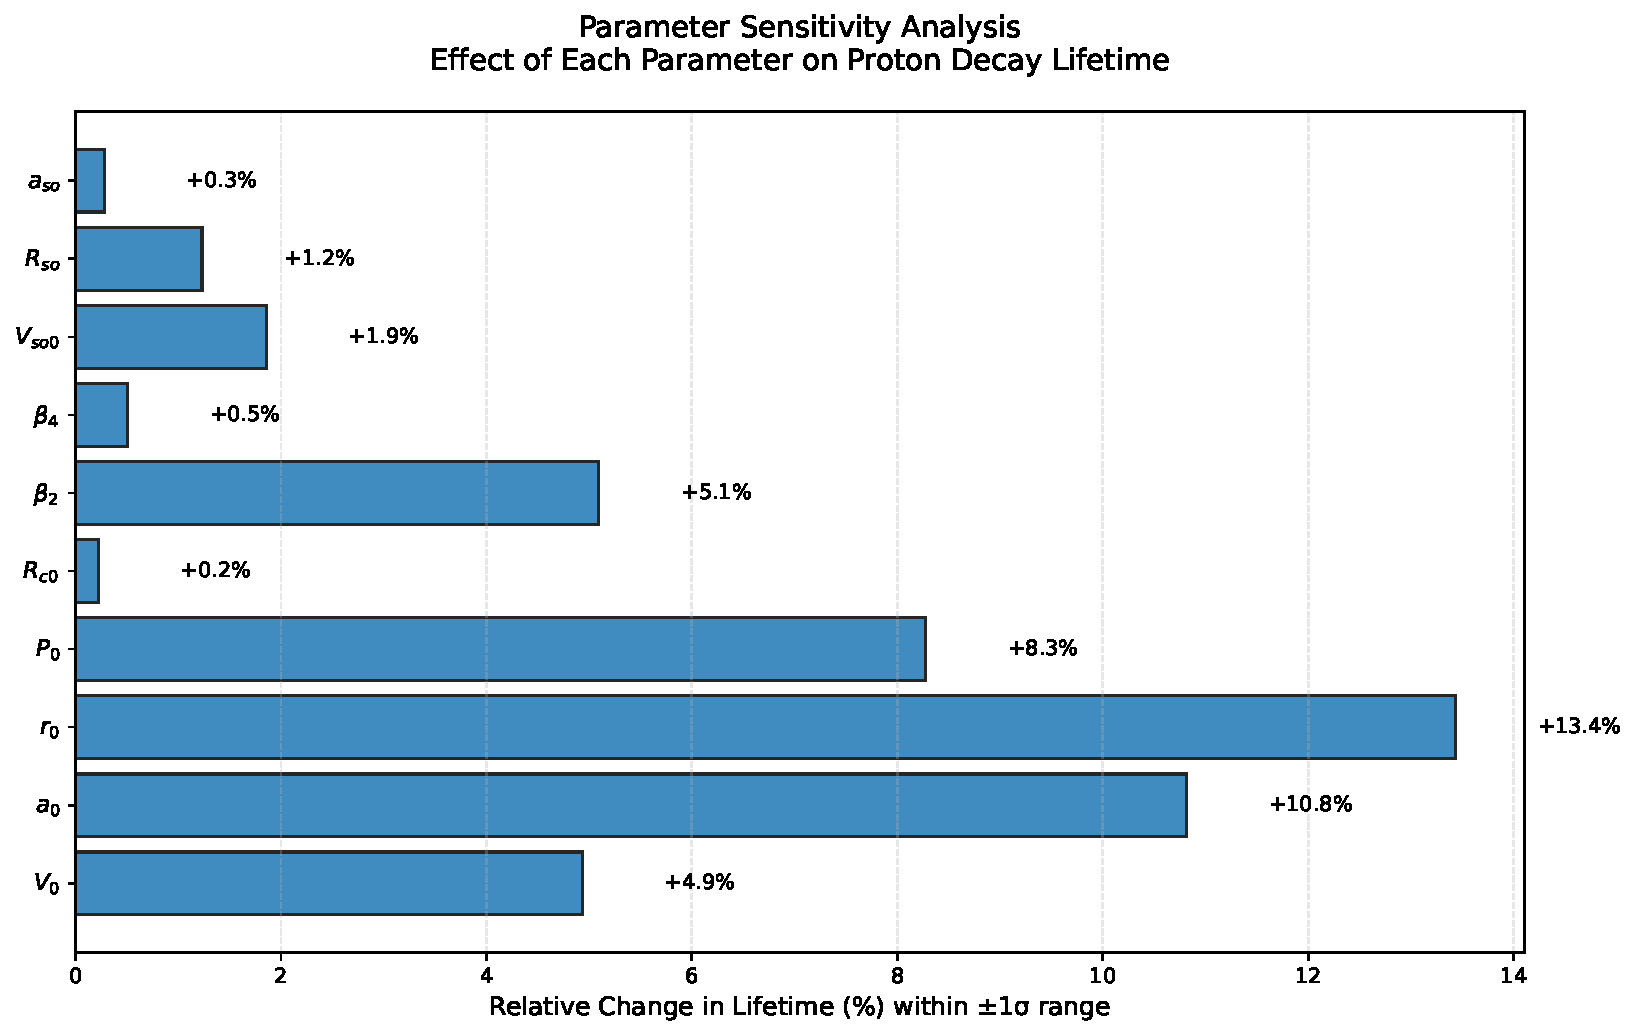
\includegraphics[width=0.8\textwidth]{Figures/figure33.pdf}
    \caption{151Lu的参数敏感性图(1sigma区间内的参数变化对半衰期的影响)}
    \label{fig:33}
\end{figure}

最后是151Lu的可观测量sigma区间：
\begin{verbatim}
========== Posterior Predictive Distribution of Lifetime ==========
experiment data: [0.079] s
Number of posterior samples used: 5000
Mean lifetime      : 7.915e-02 s
Median lifetime    : 7.916e-02 s
Standard deviation : 1.013e-03 s
1σ error bar (±)   : 1.013e-03 s
2σ error bar (±)   : 2.026e-03 s
68% CI (1σ)        : [7.813e-02, 8.014e-02] s
95% CI (2σ)        : [7.718e-02, 8.115e-02] s
===================================================================
\end{verbatim}


\clearpage
对于155Ta进行研究，选取的计算参数如下：
\begin{verbatim}    
#155Ta
e2=1.43997 ; hbarc=197.3269718 ; amu=931.49432
zp=73 ; Ap=155 ; mass_excess_p=-23.988 ; mp=Ap*amu+mass_excess_p        #Parent
z1=zp-1 ; A1=Ap-1 ; mass_excess_1=-32.730 ; m1=A1*amu+mass_excess_1    #1-> daughter
z2=1  ; A2=1   ; mass_excess_2=7.288971064 ; m2=A2*amu+mass_excess_2
Q=mp-m1-m2
print("Q=",Q)
mu=m1*m2/(m1+m2)
P0=0.422
#Potential

#Deformation
beta2 = 0.021  # quadrupole
beta4 = 0.000  # hexadecapole 

#Polarizaton
beta2tilde = 0  
beta4tilde = 0

#spin-orbit
Vso0=6.2 ; rso=1.01*(A1)**(1/3) ; aso=0.75 ; lambda_pi=np.sqrt(2)
L=5; S=0.5; J=5.5
print("rso=",rso)
#Vn
a0=0.75 ; r0=1.27*A1**(1/3)-0.1 ; V0=55
print("r0=",r0)
#Vc
Rc0 = 1.21 * A1**(1/3)          
print("Rc0=",Rc0)
#mesh
r = np.linspace(0.03, 30.0, 1000) # avoid too small r


# experiment data
y=np.array([2.9e-3])    # s
sigma=np.array([1.5e-3])


# Hyperparameters in Prior
    v0_mean=55; a0_mean=0.75; r0_mean=1.27*A1**(1/3)-0.1; p0_mean=0.422
    rc0_mean=1.21 * A1**(1/3); beta2_mean=0.021 ; beta4_mean=0.000
    vso0_mean=6.2; rso_mean=1.01*(A1)**(1/3); aso_mean=0.75
with multiprocessing.Pool() as pool:
    sampler = emcee.EnsembleSampler(nwalkers, M, log_posterior, 
    args=[y,sigma],a=2.0,pool=pool)
    state = sampler.run_mcmc(initial_positions, 200)
    sampler.reset()
    sampler.run_mcmc(state,5000)

\end{verbatim}


这里只选取了5000samples/sampler就已经收敛

获得155Ta的posterior图：  
\begin{figure}[htbp]
    \centering
    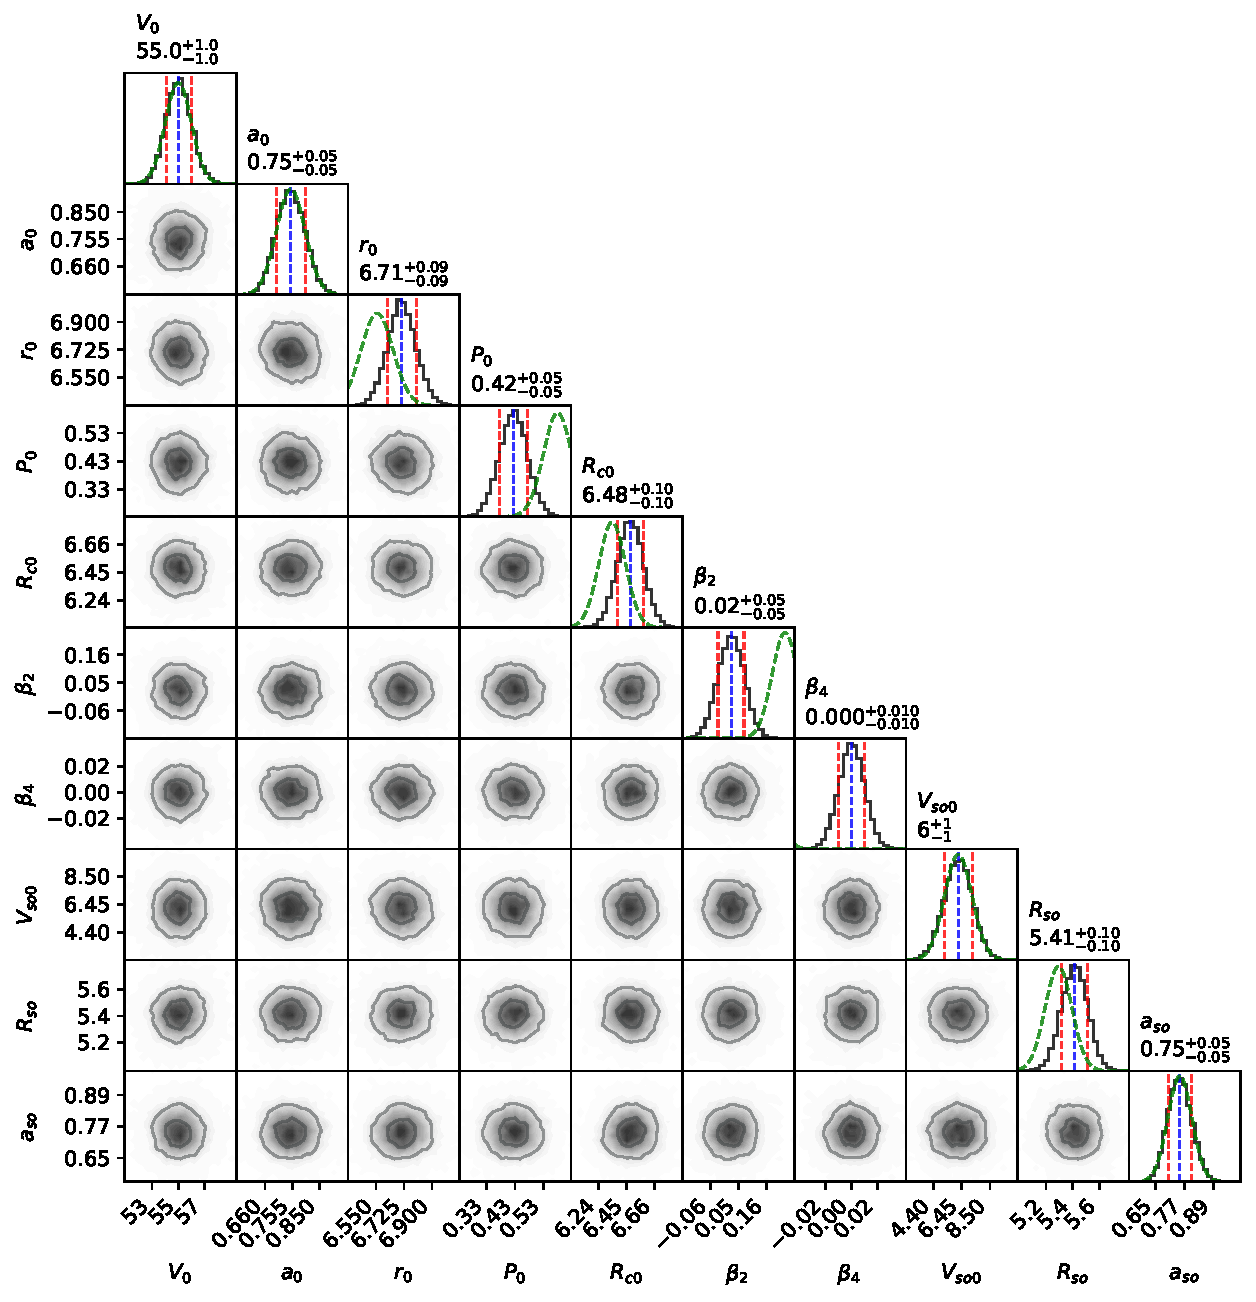
\includegraphics[width=0.8\textwidth]{Figures/figure34.pdf}
    \caption{155Ta的后验图(5000samples/sampler的正式运行)}
    \label{fig:34}
\end{figure}

然后是155Ta的参数关联图：
\begin{figure}[htbp]
    \centering
    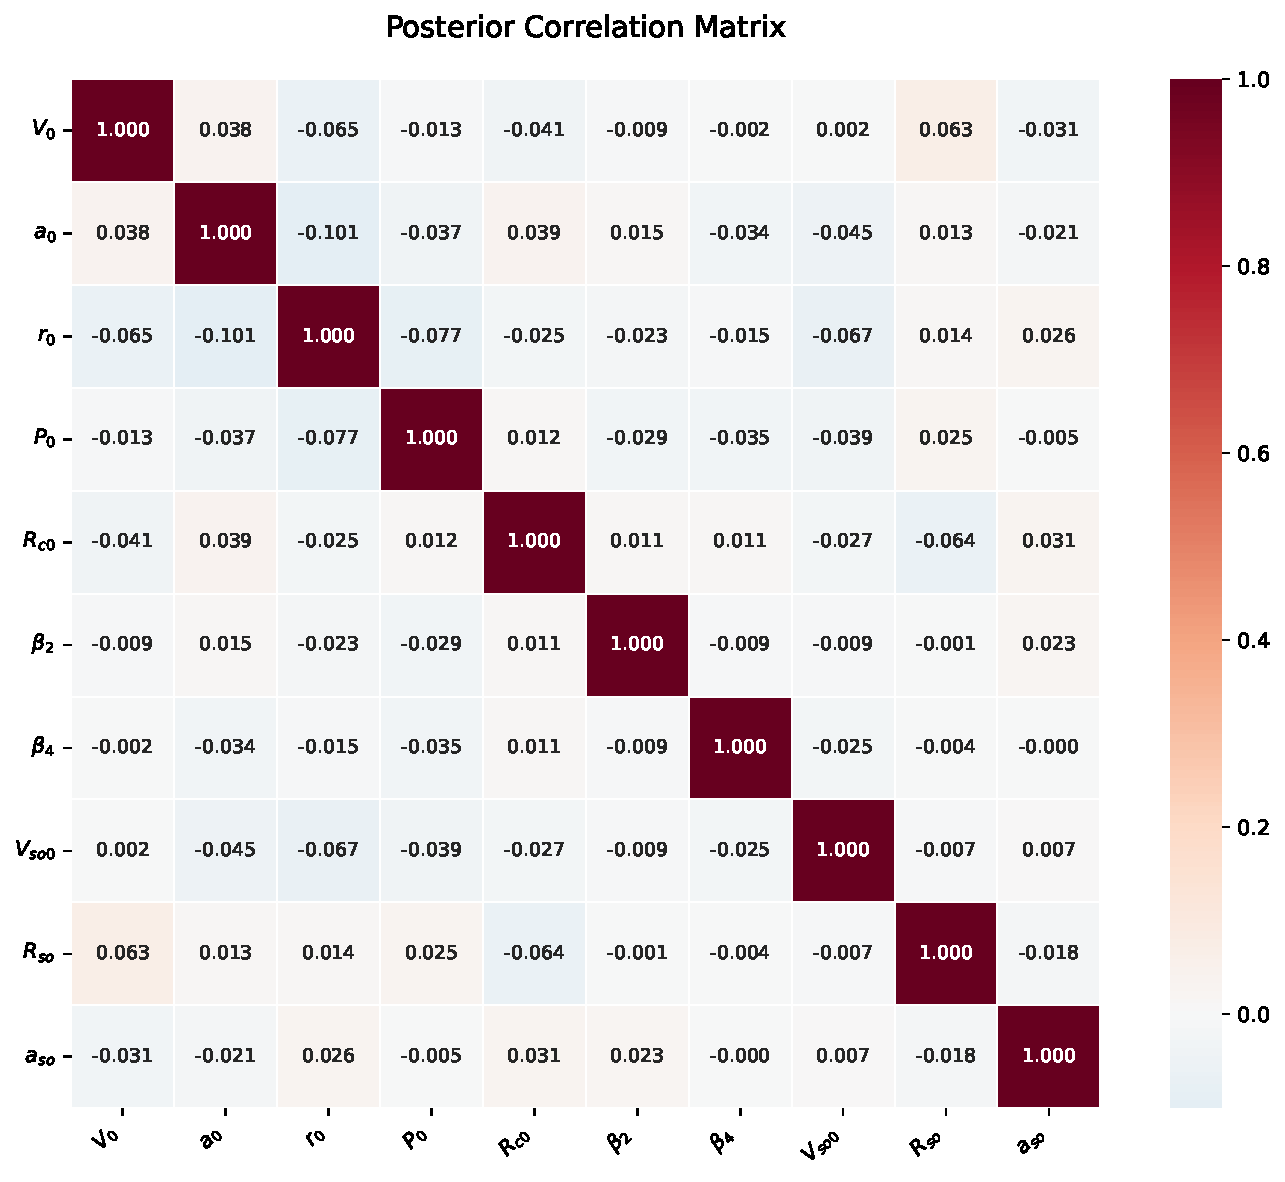
\includegraphics[width=0.8\textwidth]{Figures/figure35.pdf}
    \caption{155Ta的形变势能参数的关联矩阵}
    \label{fig:35}
\end{figure}

然后是155Ta的参数敏感性图：
\begin{figure}[htbp]
    \centering
    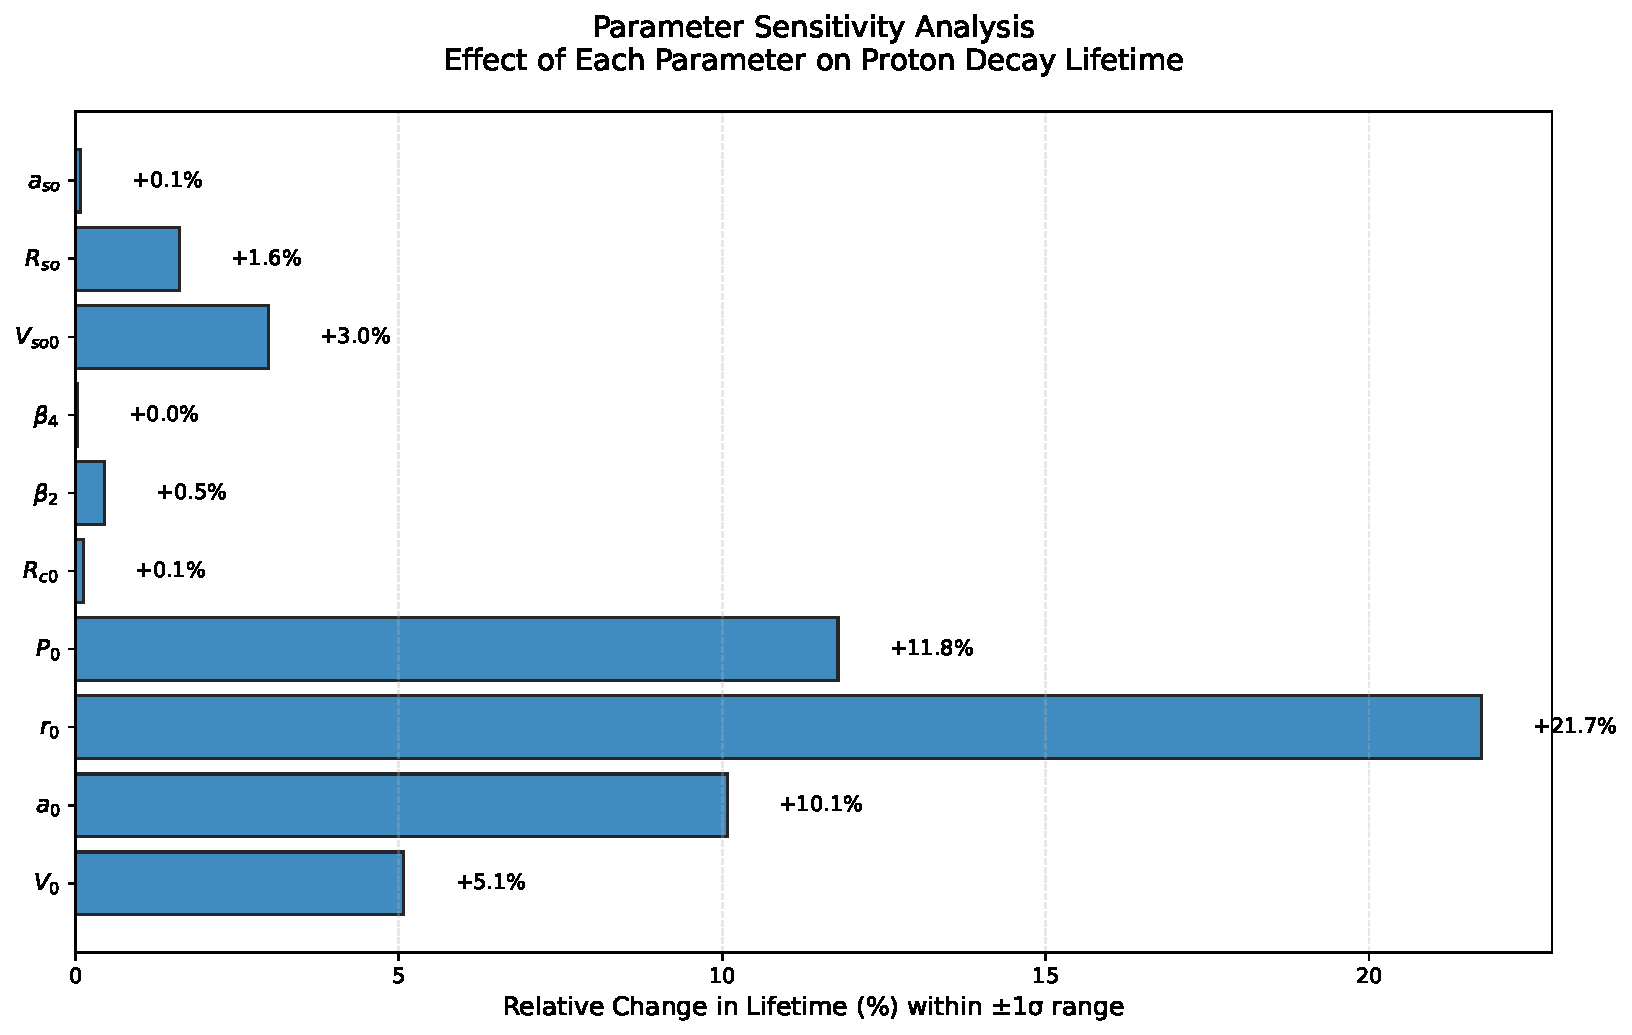
\includegraphics[width=0.8\textwidth]{Figures/figure36.pdf}
    \caption{155Ta的参数敏感性图(1sigma区间内的参数变化对半衰期的影响)}
    \label{fig:36}
\end{figure}

\clearpage

然后对161Re进行研究，选取的计算参数如下：
\begin{verbatim}
#System of Proton Decay
#161Re
e2=1.43997 ; hbarc=197.3269718 ; amu=931.49432
zp=75 ; Ap=161 ; mass_excess_p=-20.84282 ; mp=Ap*amu+mass_excess_p        #Parent
z1=zp-1 ; A1=Ap-1 ; mass_excess_1=-29.329073 ; m1=A1*amu+mass_excess_1    #1-> daughter
z2=1  ; A2=1   ; mass_excess_2=7.288971064 ; m2=A2*amu+mass_excess_2
Q=mp-m1-m2
print("Q=",Q)
mu=m1*m2/(m1+m2)
P0=0.892
#Potential

#Deformation
beta2 = 0.128  # quadrupole
beta4 = 0.018  # hexadecapole 

#Polarizaton
beta2tilde = 0  
beta4tilde = 0

#spin-orbit
Vso0=6.2 ; rso=1.01*(A1)**(1/3) ; aso=0.75 ; lambda_pi=np.sqrt(2)
L=0; S=0.5; J=0.5
print("rso=",rso)
#Vn
a0=0.75 ; r0=1.27*A1**(1/3)-0.1 ; V0=55
print("r0=",r0)
#Vc
Rc0 = 1.21 * A1**(1/3)          
print("Rc0=",Rc0)
#mesh
r = np.linspace(0.03, 30.0, 1000) # avoid too small r

# experiment data
y=np.array([0.44e-3])    # s
sigma=np.array([0.01e-3])

# Hyperparameters in Prior
    v0_mean=55; a0_mean=0.75; r0_mean=1.27*A1**(1/3)-0.1; p0_mean=P0
    rc0_mean=1.21 * A1**(1/3); beta2_mean=beta2 ; beta4_mean=beta4
    vso0_mean=6.2; rso_mean=1.01*(A1)**(1/3); aso_mean=0.75

    sampler = emcee.EnsembleSampler(nwalkers, M, log_posterior, 
    args=[y,sigma],a=2.0,pool=pool)
    state = sampler.run_mcmc(initial_positions, 200)
    sampler.reset()
    sampler.run_mcmc(state,10000)
\end{verbatim}
\clearpage
获得了161Re的posterior图：
\begin{figure}[htbp]
    \centering
    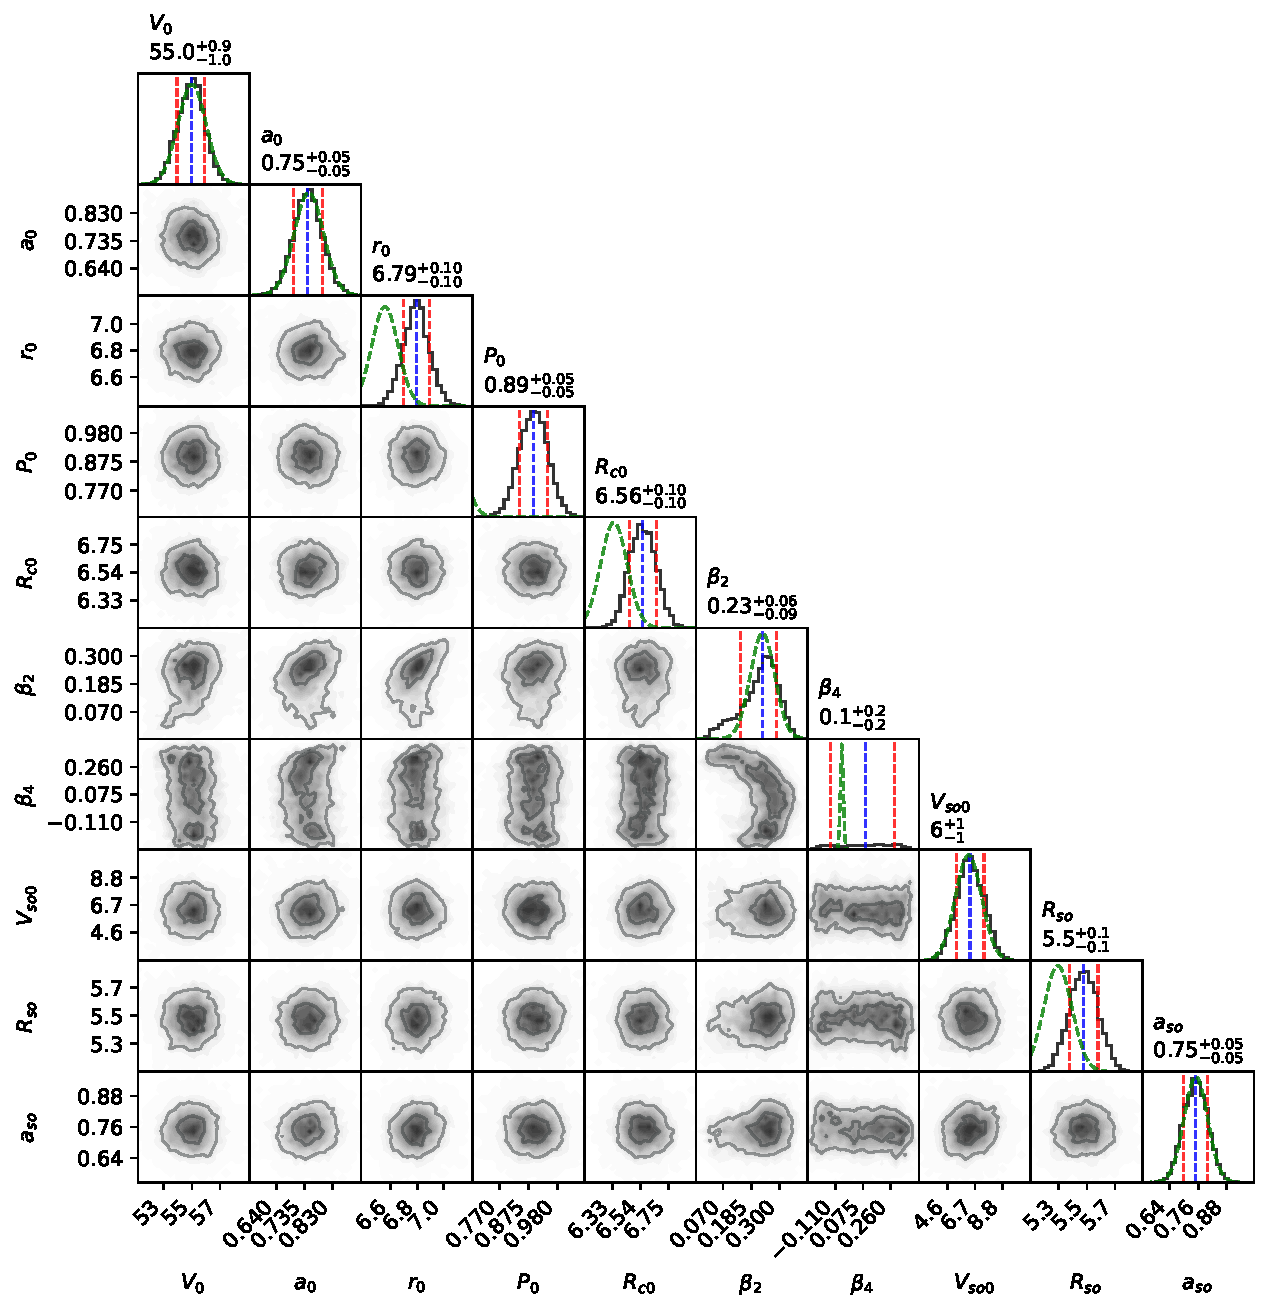
\includegraphics[width=0.8\textwidth]{Figures/figure37.pdf}
    \caption{161Re的后验图(10000samples/sampler的正式运行)}
    \label{fig:37}
\end{figure}

然后是161Re的参数关联图：
\begin{figure}[htbp]
    \centering
    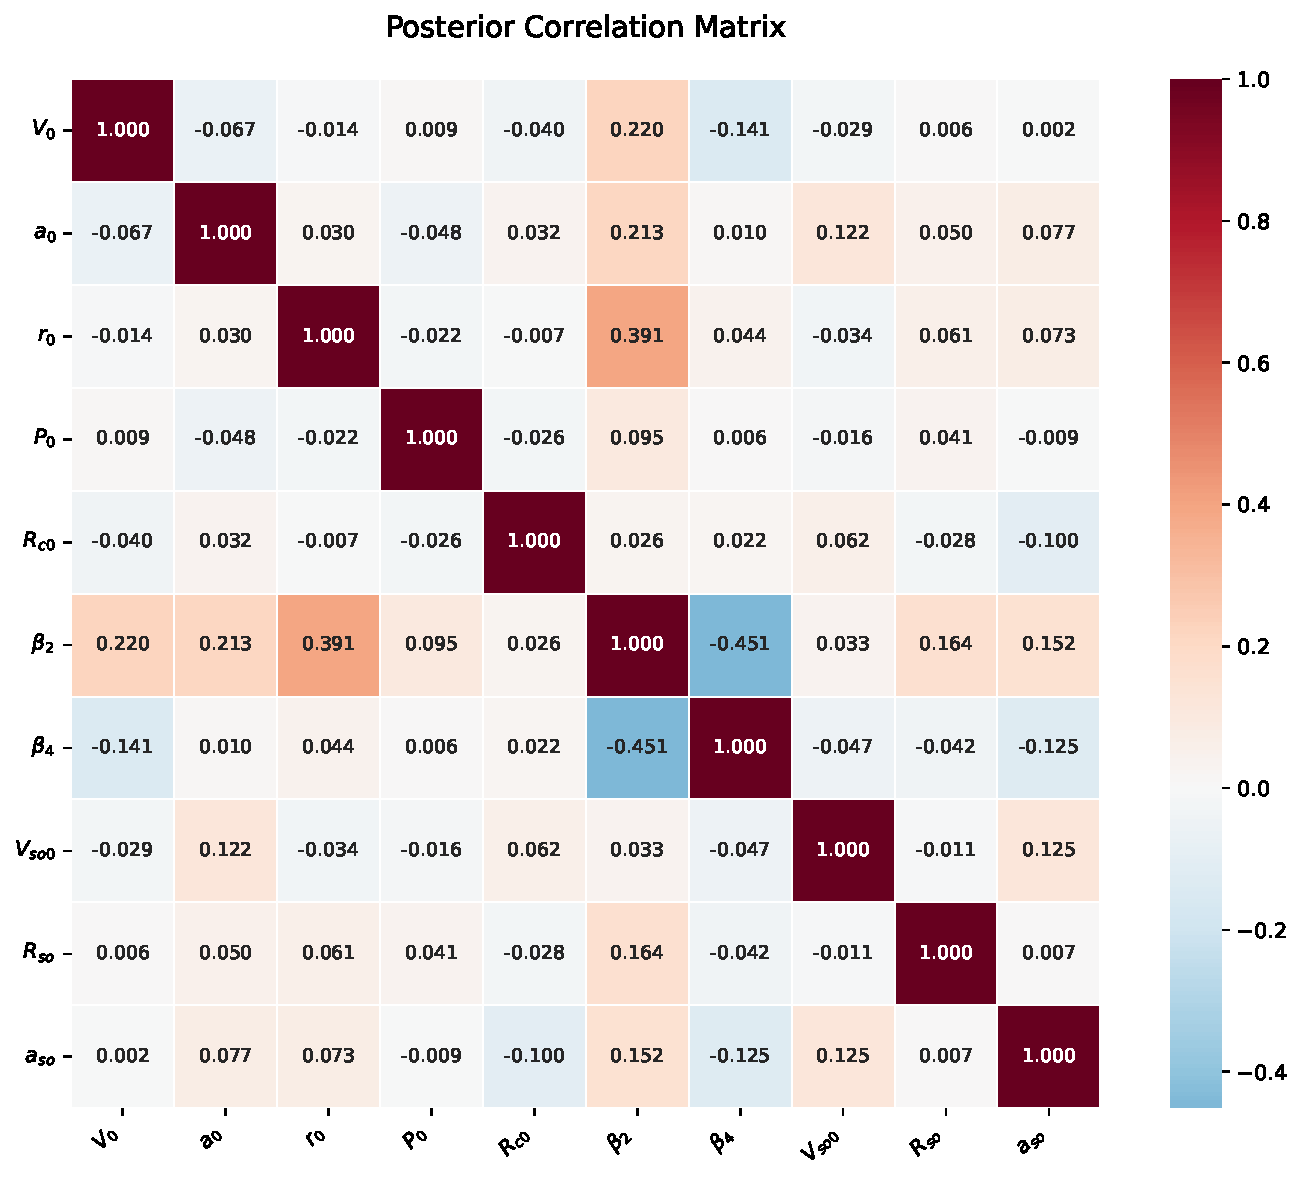
\includegraphics[width=0.8\textwidth]{Figures/figure38.pdf}
    \caption{161Re的形变势能参数的关联矩阵}
    \label{fig:38}
\end{figure}


然后是161Re的参数敏感性图：
\begin{figure}[htbp]
    \centering
    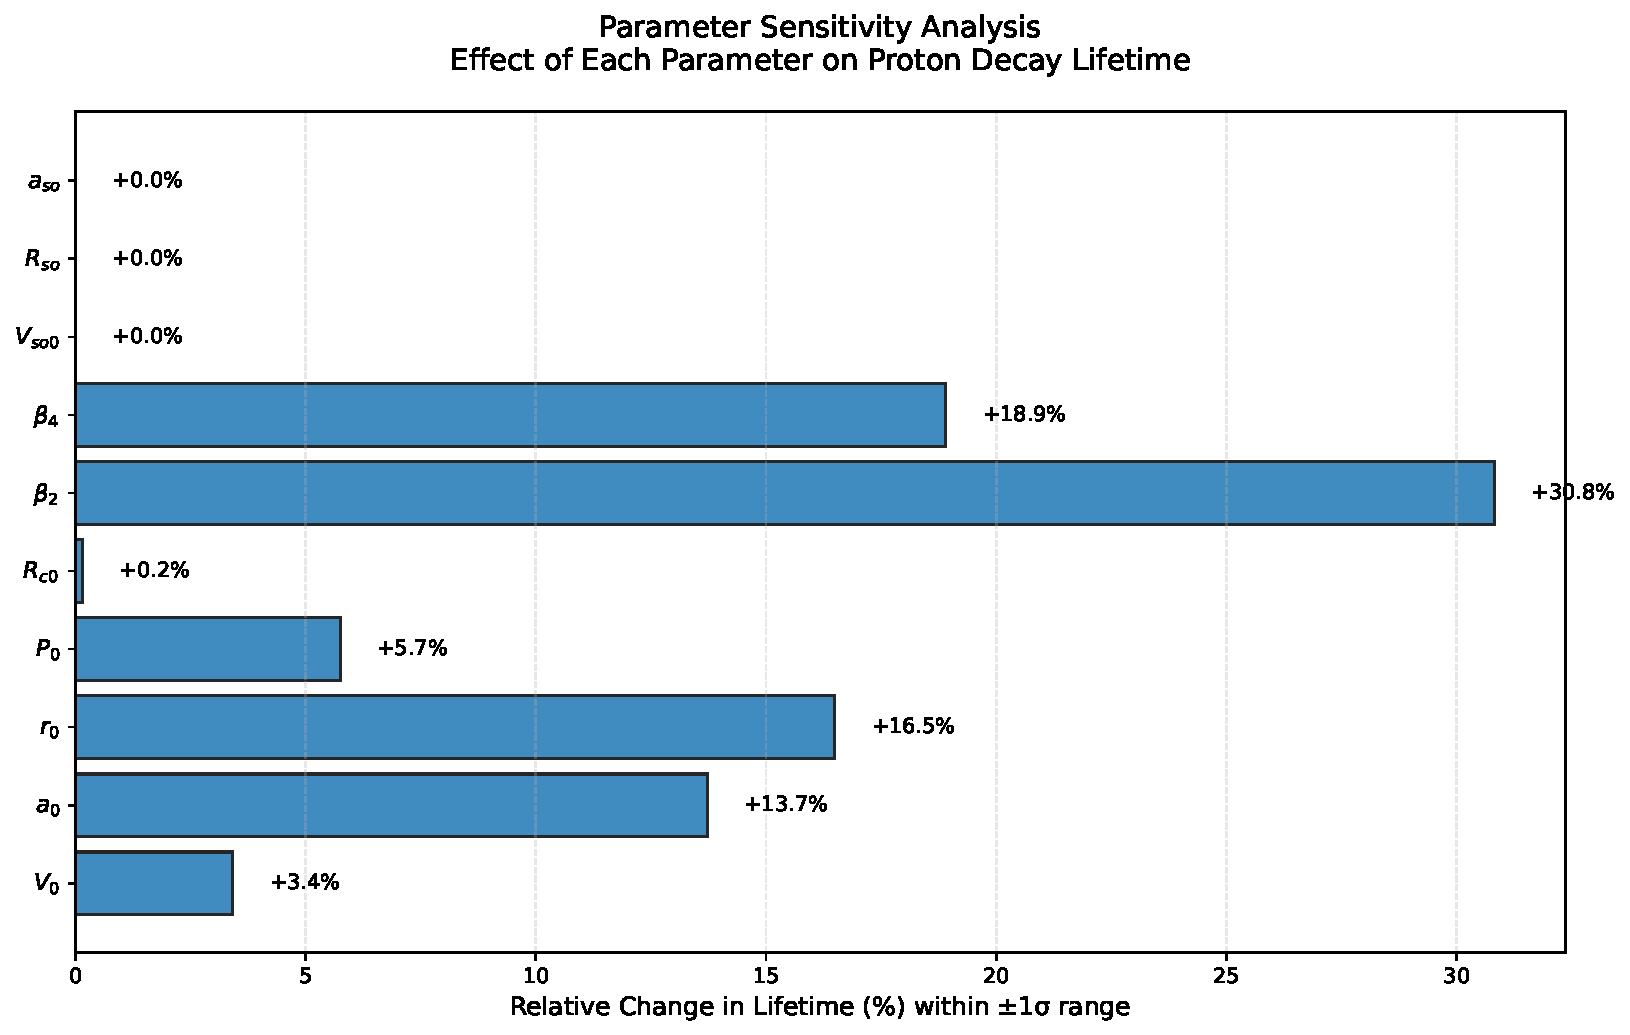
\includegraphics[width=0.8\textwidth]{Figures/figure39.pdf}
    \caption{161Re的参数敏感性图(1sigma区间内的参数变化对半衰期的影响)}
    \label{fig:39}
\end{figure}

最后是161Re的可观测量sigma区间：
\begin{verbatim}
========== Posterior Predictive Distribution of Lifetime ==========
experiment data: [0.00044] s
Number of posterior samples used: 5000
Mean lifetime      : 4.401e-04 s
Median lifetime    : 4.402e-04 s
Standard deviation : 9.992e-06 s
1σ error bar (±)   : 9.992e-06 s
2σ error bar (±)   : 1.998e-05 s
68% CI (1σ)        : [4.301e-04, 4.500e-04] s
95% CI (2σ)        : [4.205e-04, 4.596e-04] s
===================================================================
\end{verbatim}

\clearpage

前面的图中prior曲线作图的时候有参数问题，后进行修改（但所有的input均没问题， 记录在前面了）


我们继续记录其他的input


对于165Ir进行研究，这里发生质子衰变的165Ir是一个激发态
\begin{figure}[htbp]
    \centering
    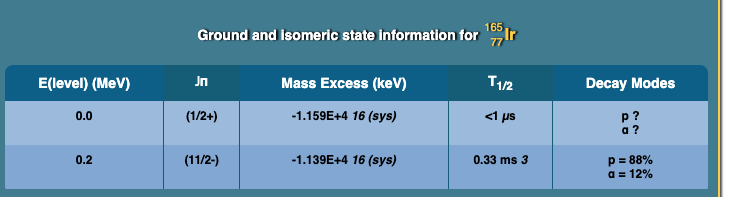
\includegraphics[width=0.8\textwidth]{Figures/figure40.png}
    \caption{165Ir的核数据，应选取11/2-的激发态进行计算}
    \label{fig:40}
\end{figure}

我们标记为$^{165}\mathrm{Ir}_m$，记录input如下
\begin{verbatim}
#System of Proton Decay
#165Irm(excited state)
e2=1.43997 ; hbarc=197.3269718 ; amu=931.49432
zp=77 ; Ap=165 ; mass_excess_p=-11.39 ; mp=Ap*amu+mass_excess_p        #Parent
z1=zp-1 ; A1=Ap-1 ; mass_excess_1=-20.424723 ; m1=A1*amu+mass_excess_1    #1-> daughter
z2=1  ; A2=1   ; mass_excess_2=7.288971064 ; m2=A2*amu+mass_excess_2
Q=mp-m1-m2
print("Q=",Q)
mu=m1*m2/(m1+m2)
P0=0.187
#Potential

#Deformation
beta2 = 0.129  # quadrupole
beta4 = 0.006  # hexadecapole 

#Polarizaton
beta2tilde = 0  
beta4tilde = 0

#spin-orbit
Vso0=6.2 ; rso=1.01*(A1)**(1/3) ; aso=0.75 ; lambda_pi=np.sqrt(2)
L=5; S=0.5; J=5.5
print("rso=",rso)
#Vn
a0=0.75 ; r0=1.27*A1**(1/3)-0.1 ; V0=55
print("r0=",r0)
#Vc
Rc0 = 1.21 * A1**(1/3)          
print("Rc0=",Rc0)
#mesh
r = np.linspace(0.03, 30.0, 1000) # avoid too small r

# experiment data
y=np.array([0.33e-3])    # s
sigma=np.array([0.03e-3])

# Hyperparameters in Prior
    v0_mean=55; a0_mean=0.75; r0_mean=1.27*A1**(1/3)-0.1; p0_mean=P0
    rc0_mean=1.21 * A1**(1/3); beta2_mean=beta2 ; beta4_mean=beta4
    vso0_mean=6.2; rso_mean=1.01*(A1)**(1/3); aso_mean=0.75


    with multiprocessing.Pool() as pool:
    sampler = emcee.EnsembleSampler(nwalkers, M, log_posterior, 
    args=[y,sigma],a=2.0,pool=pool)
    state = sampler.run_mcmc(initial_positions, 200)
    sampler.reset()
    sampler.run_mcmc(state,10000)
\end{verbatim}


使用上述input 计算已经收敛

然后记录171Au的计算参数如下：
\begin{verbatim}
#System of Proton Decay
#171Au
e2=1.43997 ; hbarc=197.3269718 ; amu=931.49432
zp=79 ; Ap=171 ; mass_excess_p=-7.562303 ; mp=Ap*amu+mass_excess_p        #Parent
z1=zp-1 ; A1=Ap-1 ; mass_excess_1=-16.299202 ; m1=A1*amu+mass_excess_1    #1-> daughter
z2=1  ; A2=1   ; mass_excess_2=7.288971064 ; m2=A2*amu+mass_excess_2
Q=mp-m1-m2
print("Q=",Q)
mu=m1*m2/(m1+m2)
P0=0.848
#Potential

#Deformation
beta2 = 0.129  # quadrupole
beta4 = -0.006  # hexadecapole 

#Polarizaton
beta2tilde = 0  
beta4tilde = 0

#spin-orbit
Vso0=6.2 ; rso=1.01*(A1)**(1/3) ; aso=0.75 ; lambda_pi=np.sqrt(2)
L=0; S=0.5; J=0.5
print("rso=",rso)
#Vn
a0=0.75 ; r0=1.27*A1**(1/3)-0.1 ; V0=55
print("r0=",r0)
#Vc
Rc0 = 1.21 * A1**(1/3)          
print("Rc0=",Rc0)
#mesh
r = np.linspace(0.03, 30.0, 1000) # avoid too small r


# experiment data
y=np.array([22e-6])    # s
sigma=np.array([3e-6])

# Hyperparameters in Prior
    v0_mean=55; a0_mean=0.75; r0_mean=1.27*A1**(1/3)-0.1; p0_mean=P0
    rc0_mean=1.21 * A1**(1/3); beta2_mean=beta2 ; beta4_mean=beta4
    vso0_mean=6.2; rso_mean=1.01*(A1)**(1/3); aso_mean=0.75
    

with multiprocessing.Pool() as pool:
    sampler = emcee.EnsembleSampler(nwalkers, M, log_posterior, 
    args=[y,sigma],a=1.0,pool=pool)
    state = sampler.run_mcmc(initial_positions, 200)
    sampler.reset()
    sampler.run_mcmc(state,10000)
\end{verbatim}

所有的sigma区间信息包含在了output文件中。

然后记录176Tl的计算参数如下：
其中176Tl的质子的L取0（nndc上的信息）
\begin{verbatim}
#System of Proton Decay
#176Tl
e2=1.43997 ; hbarc=197.3269718 ; amu=931.49432
zp=81 ; Ap=176 ; mass_excess_p=0.584728 ; mp=Ap*amu+mass_excess_p        #Parent
z1=zp-1 ; A1=Ap-1 ; mass_excess_1=-7.969443; m1=A1*amu+mass_excess_1    #1-> daughter
z2=1  ; A2=1   ; mass_excess_2=7.288971064 ; m2=A2*amu+mass_excess_2
Q=mp-m1-m2
print("Q=",Q)
mu=m1*m2/(m1+m2)
P0=0.926
#Potential

#Deformation
beta2 = -0.115  # quadrupole
beta4 = -0.030  # hexadecapole 

#Polarizaton
beta2tilde = 0  
beta4tilde = 0

#spin-orbit
Vso0=6.2 ; rso=1.01*(A1)**(1/3) ; aso=0.75 ; lambda_pi=np.sqrt(2)
L=0; S=0.5; J=0.5
print("rso=",rso)
#Vn
a0=0.75 ; r0=1.27*A1**(1/3)-0.1 ; V0=55
print("r0=",r0)
#Vc
Rc0 = 1.21 * A1**(1/3)          
print("Rc0=",Rc0)
#mesh
r = np.linspace(0.03, 30.0, 1000) # avoid too small r

# experiment data
y=np.array([5.2e-3])    # s
sigma=np.array([3e-3])

# Hyperparameters in Prior
    v0_mean=55; a0_mean=0.75; r0_mean=1.27*A1**(1/3)-0.1; p0_mean=P0
    rc0_mean=1.21 * A1**(1/3); beta2_mean=beta2 ; beta4_mean=beta4
    vso0_mean=6.2; rso_mean=1.01*(A1)**(1/3); aso_mean=0.75

    
with multiprocessing.Pool() as pool:
    sampler = emcee.EnsembleSampler(nwalkers, M, log_posterior, 
    args=[y,sigma],a=2.0,pool=pool)
    state = sampler.run_mcmc(initial_positions, 200)
    sampler.reset()
    sampler.run_mcmc(state,10000)

\end{verbatim}



\appendix
\chapter{Supplementary Calculations}
Put detailed derivations that are too long for the main text here.

\end{document}
